%%%% Various options for document class.
%DIF LATEXDIFF DIFFERENCE FILE
%DIF DEL compare.tex   Tue Nov 10 16:44:34 2015
%DIF ADD paper.tex     Thu Nov 12 10:15:19 2015
%%\documentclass[usenatbib, a4paper, 11pt]{aastex}
%%\documentclass[preprint, 11pt, a4paper]{aastex}
%%\documentclass[twocolum]{revtex4}
%%\documentclass{report}
%\documentclass[useAMS,usenatbib]{mn2e_x}
\documentclass[preprint, a4paper, 11pt]{aastex}
%\usepackage{psfig,morefloats,url}
%use preprint2 for 2 columns paper.

%% declare any packages used
\usepackage{graphicx}
\usepackage{natbib}
\usepackage{graphicx}
\usepackage{color}
\usepackage{pdfpages}
\usepackage{appendix}
\usepackage{subfigure}
\usepackage{url}
%DIF 20a20
\usepackage{amsmath} %DIF > 
%DIF -------
%\usepackage{pngfig}
%DIF 21c22
%DIF < %\usepackage[dvips]{color}
%DIF -------
%\usepackage[dvips]{color}mak %DIF > 
%DIF -------
%\usepackage{aabib}


%\marginparwidth = 25pt
\citestyle{aa}
\addtolength{\topmargin}{-.5in}
%\addtolength{\bottommargin}{-1in}
%% This command added as margins are wrong in mn2e, it appears. 
%% Not needed for other classes
\usepackage{float}



%%%%%%%%%%%%%%%%%%%%%%%%%%%%%%%%%%%%%%
%DIF PREAMBLE EXTENSION ADDED BY LATEXDIFF
%DIF UNDERLINE PREAMBLE %DIF PREAMBLE
\RequirePackage[normalem]{ulem} %DIF PREAMBLE
\RequirePackage{color}\definecolor{RED}{rgb}{1,0,0}\definecolor{BLUE}{rgb}{0,0,1} %DIF PREAMBLE
\providecommand{\DIFadd}[1]{{\protect\color{blue}\uwave{#1}}} %DIF PREAMBLE
\providecommand{\DIFdel}[1]{{\protect\color{red}\sout{#1}}}                      %DIF PREAMBLE
%DIF SAFE PREAMBLE %DIF PREAMBLE
\providecommand{\DIFaddbegin}{} %DIF PREAMBLE
\providecommand{\DIFaddend}{} %DIF PREAMBLE
\providecommand{\DIFdelbegin}{} %DIF PREAMBLE
\providecommand{\DIFdelend}{} %DIF PREAMBLE
%DIF FLOATSAFE PREAMBLE %DIF PREAMBLE
\providecommand{\DIFaddFL}[1]{\DIFadd{#1}} %DIF PREAMBLE
\providecommand{\DIFdelFL}[1]{\DIFdel{#1}} %DIF PREAMBLE
\providecommand{\DIFaddbeginFL}{} %DIF PREAMBLE
\providecommand{\DIFaddendFL}{} %DIF PREAMBLE
\providecommand{\DIFdelbeginFL}{} %DIF PREAMBLE
\providecommand{\DIFdelendFL}{} %DIF PREAMBLE
%DIF END PREAMBLE EXTENSION ADDED BY LATEXDIFF

\begin{document}
%% define bibstyle and other definitions
\bibliographystyle{aabib}
%% renew commands
%%\renewcommand{\labelitemi}{$.$}

%% Codes
\def\py{\textsc{Python}}
\def\tar{\textsc{Tardis}}
\def\cld{\textsc{Cloudy}}
\def\agn{\textsc{Agnspec}}


%% Lines and ions
\def\civ{C~\textsc{iv}}
\def\nv{N~\textsc{v}}
\def\hei{He~\textsc{i}}
\def\heii{He~\textsc{ii}}
\def\mg{Mg~\textsc{ii}}
\def\al{Al~\textsc{iii}}
\def\heii{He~\textsc{ii}}
\def\ovi{O~\textsc{vi}}
\def\la{Ly~$\alpha$}
\def\ha{H~$\alpha$}
\def\hb{H~$\beta$}



%% Journal definitions
\def\araa{ARAA}
\def\nat{Nature}
\def\apjl{ApJ Letters}
\def\aapr{AAPR}
\def\ssr{SSR}
\def\apj{ApJ}
\def\apjs{ApJs}
\def\pasp{PASP}
\def\aap{A\&A}
\def\mnras{MNRAS}
\def\aj{AJ}
\def\rmxaa{RMXAA}
\def\aaps{A\&As}
\DIFaddbegin \def\LA{Lyman\thinspace$\alpha$}
\DIFaddend 

\DIFaddbegin \newcommand{\EXPN}[2]{\mbox{$#1\times 10^{#2}$}}
\newcommand{\EXPU}[3]{\mbox{\rm $#1 \times 10^{#2} \rm\:#3$}}  %DIF >  exponent with units
\newcommand{\POW}[2]{\mbox{$\rm10^{#1}\rm\:#2$}}
\def\LUM{\:{\rm ergs\:s^{-1}}}
\def\FLUX{\:{\rm ergs\:cm^{-2}\:s^{-1}}}
\def\OIGS{\:{\rm ergs\:cm^{-2}\:s^{-1}\:\AA^{-1}}}

\DIFaddend %%%%%%%%%%%%%%%%%%%%%%%%%%%%%%%%%%%%%%
%
%          TITLE AND AUTHORS
%
%%%%%%%%%%%%%%%%%%%%%%%%%%%%%%%%%%%%%%%

\title
{
% Modelling quasar outflows:
% clumpy winds and broad emission lines
\DIFdelbegin \DIFdel{Unifying quasars with clumpy wind models
}\DIFdelend \DIFaddbegin \DIFadd{Testing Quasar Unification with Clumpy Wind Models
%DIF > Unifying quasars with clumpy wind models
}\DIFaddend }


%DIF <  [Matthews, J.]
%DIF <  \author[Matthews, J.]{James Matthews \\
%DIF <  {\sl  Supervisor: Prof. Christian Knigge} \\
%DIF <  {\sl School of Physics \& Astronomy, University of Southampton,
%DIF <    Southampton, SO17 1BJ, UK}}
\DIFdelbegin %DIFDELCMD < 

%DIFDELCMD < %%%
\DIFdelend %\author[Matthews et al.]
\author{\DIFdelbegin \DIFdel{
\parbox[t]{\textwidth}{
J.~H.~Matthews$^1$\thanks{jm8g08@soton.ac.uk}, C.~Knigge$^1$,
N.~Higginbottom$^1$, K.~S.~Long$^2$, S.~A.~Sim$^3$ and S.~W.~Mangham$^1$
}
}\DIFdelend \DIFaddbegin \DIFadd{
\parbox[t]{\textwidth}{
James~H.~Matthews$^1$\thanks{jm8g08@soton.ac.uk}, Christian~Knigge$^1$,
Nick~Higginbottom$^1$, Knox~S.~Long$^2$, Stuart~A.~Sim$^3$ and Sam~W.~Mangham$^1$
}
}\DIFaddend \medskip  
\\$^1$School of Physics and Astronomy, University of Southampton, Highfield, Southampton, SO17 1BJ, United Kingdom
\\$^2$Space Telescope Science Institute, 3700 San Martin Drive, Baltimore, MD, 21218
\\$^3$School of Mathematics and Physics, Queens University Belfast, University Road, Belfast, BT7 1NN, Northern Ireland, UK
}





\date{\today}
%\\
%Supervisor: Prof. Christian Knigge\\
%{\sl School of Physics \& Astronomy, University of Southampton,
%  Southampton, SO17 1BJ, UK}}


%%%%%%%%%%%%%%%%%%%%%%%%%%%%%%%%%%%%%%
%
%          ABSTRACT
%
%%%%%%%%%%%%%%%%%%%%%%%%%%%%%%%%%%%%%%%




\begin{abstract} 
% Broad absorption lines (BALs) in the ultraviolet 
% are seen in $\sim20\%$ of quasi-stellar objects (QSOs). 
% Blue-shifted broad absorption lines (BALs) are the most direct evidence of 
% accretion disc `winds' in such systems; mass loaded outflows
% emanating from the disc that may be driven by line forces or
% magnetic processes. 
% Various unification schemes for
% quasars and luminous active galactic nuclei (AGN) have proposed
% that the broad emission line region is roughly cospatial
% with broad absorption line (BAL) gas and much of the phenomenology of luminous AGN
% can be explained by a simple geometrical picture involving an accretion
% disc and associated outflow. Here, we test this paradigm by 
% utilising our state-of-the-art radiative transfer code to produce synthetic spectra
% from simple biconical disc wind models. 
% In particular, we expand on our previous 
% work in which a benchmark model for BAL quasars was produced. 
% We have conducted a limited parameter search with the aim of unifying quasar phenomenology,
% and arrive at an improved model. The grid is now publicly available.
% We find that a simple treatment of clumping (`microclumping') 
% allows for a more realistic X-ray luminosity in the model by lowering the 
% ionization parameter. We examine the X-ray properties of this new model
% and find good agreement with existing X-ray samples of AGN and QSOs.
% We find that the dense, X-ray heated wind 
% produces strong H recombination and collisionally excited resonance 
% line emission to emerge at the low inclination angles, 
% which represent quasars within this unification scenario.
% % We also treat Hydrogen using a `macro-atom' approach in order to 
% % examine the effect of recombination on Hydrogen emission lines, and
% % this results in significant line emission in Lyman~$\alpha$ and the Balmer series.
% However, we are unable to reproduce the remarkably similar of line-to-continuum
% ratios between BAL and non-BAL quasar composites.
% This is due to a fundamental constraint arising
% from the anisotropy of emission from a classical thin disc. 
% We briefly explore the effect of relativistic beaming, gravitational redshift and 
% light bending on the angular distribution of disc continuum emission. 
% We find that these general relativistic effects do cause the disc to
% emit slightly more isotropically, but this is not yet sufficient to produce a
% self-consistent model. We discuss wind reprocessing as a potential solution.
% Overall, our work suggests that geometric unification
% involving an accretion disc wind is a promising scenario, but our results 
% pose a number of difficult challenges to such a model.
% Determining the true geometry of ADWs and uncovering the true disc spectral 
% (and angular) energy distribution are key next stpng if we are to build up a 
% holistic picture of the quasar population.
Various unification schemes \DIFdelbegin \DIFdel{for }\DIFdelend \DIFaddbegin \DIFadd{have been proposed to interpret the complex phenomenology 
of }\DIFaddend quasars and luminous active galactic nuclei (AGN) \DIFdelbegin \DIFdel{propose that much of  their complex phenomenology can be explained by a simple geometrical picture involving }\DIFdelend \DIFaddbegin \DIFadd{in terms of  a simple axisymmetric 
picture involving a central black hole, }\DIFaddend an accretion disc and \DIFaddbegin \DIFadd{an }\DIFaddend associated outflow.
Here, we \DIFdelbegin \DIFdel{test }\DIFdelend \DIFaddbegin \DIFadd{continue our tests of  }\DIFaddend this paradigm by \DIFdelbegin \DIFdel{utilising our state-of-the-art radiative transfer 
and photoionization code to 
produce synthetic spectra from }\DIFdelend \DIFaddbegin \DIFadd{comparing ``average'' quasar spectra to 
synthetic spectra of }\DIFaddend simple biconical disc wind models\DIFaddbegin \DIFadd{, using our state-of-the-art 
Monte Carlo radiative transfer and photoionization code}\DIFaddend .
In particular, we \DIFdelbegin \DIFdel{expand on our previous work by presenting a model that
exhibits many of the spectral features expected from a quasar unification model}\DIFdelend \DIFaddbegin \DIFadd{investigate whether clumping of the outflow allows us to 
produce synthetic spectra in the rest-frame UV that have the characteristics of quasars}\DIFaddend . 
We find that a simple treatment of clumping (`microclumping') 
allows for a more realistic X-ray \DIFdelbegin \DIFdel{luminosity in the model}\DIFdelend \DIFaddbegin \DIFadd{luminosities}\DIFaddend , while maintaining the ionization 
state necessary for strong BAL features \DIFaddbegin \DIFadd{in the rest-frame UV}\DIFaddend . 
We examine the X-ray properties of \DIFdelbegin \DIFdel{this new model
}\DIFdelend \DIFaddbegin \DIFadd{these simple clumped models
}\DIFaddend and find good agreement with existing X-ray samples of AGN and quasars.
\DIFdelbegin \DIFdel{We find that the }\DIFdelend \DIFaddbegin \DIFadd{The }\DIFaddend dense, X-ray heated wind produces strong recombination and collisionally 
excited line emission in, e.g., \civ\ and \la, to emerge at the low inclination, 
`Type 1 quasar-like' angles. 
\DIFdelbegin \DIFdel{The highest inclination models }\DIFdelend \DIFaddbegin \DIFadd{At the highest inclinations, the synthetic spectra }\DIFaddend possess prominent \mg\ and \al\ BALs, the absorption features seen in LoBAL quasars. 
Despite these successes, we are unable to reproduce 
the remarkably uniform emission line properties 
%DIF <  remarkably similar of line-to-continuum ratios apparent 
seen in BAL and non-BAL quasar composites. 
%DIF >  {\bf This sentence needs to be more precise, especially in 
%DIF >  light of the statement earlier in the abstract about ``good agreement''}
This is due to a fundamental constraint arising
from the anisotropy of emission from a classical thin disc. 
\DIFdelbegin \DIFdel{We briefly explore the impact of general relativistic effects
on the angular distribution of disc continuum emission, and find that 
they are not sufficient to produce a self-consistent model.
%DIF <  relativistic beaming, gravitational redshift and 
%DIF <  light bending on the angular distribution of disc continuum emission. 
%DIF <  We find that these general relativistic effects are not yet sufficient to produce a
%DIF <  self-consistent model. 
}\DIFdelend Overall, our work suggests that geometric unification
involving an accretion disc wind is a promising scenario, but our results 
pose a number of difficult challenges to such a model.
%DIF >  {\bf There is confusion in the abstract, at least, in what is the model and what is the synthetic spectra, as well as whether there is one model or many models.  We need to try to be clear.  The model should be a clumped biconical outflow.  There are then particular instantiations of the model. And then there are synthetic spectra}
\end{abstract}

\maketitle
%\begin{keywords}
%AGN: outflows
%\end{keywords}



%%%%%%%%%%%%%%%%%%%%%%%%%%%%%%%%%%%%%%
%
%          INTRODUCTION
%
%%%%%%%%%%%%%%%%%%%%%%%%%%%%%%%%%%%%%%%

\section{Introduction}

%DIF <  Introduction focussing on key points
%DIF <  \begin{itemize}
%DIF <  \item standard wind + BALQSO introduction
%DIF <  \item focus on unification and that we are testing it
%DIF <  \item some discussion of scales, referencing e.g. reverb maps, variability, microlensing, Arav 
%DIF <  \item clumping background: stellar winds, clumping in AGN winds, variability
%DIF <  \end{itemize}
\DIFdelbegin %DIFDELCMD < 

%DIFDELCMD < %%%
\DIFdelend The spectra of 
quasars and luminous active galactic nuclei (AGN) 
typically exhibit a series of strong emission lines
with an underlying blue continuum - the so-called {\sl `big blue bump'} (BBB). 
The BBB is often attributed to \DIFdelbegin \DIFdel{emssion }\DIFdelend \DIFaddbegin \DIFadd{emission }\DIFaddend from a 
geometrically thin, optically thick accretion disc surrounding the central black hole, similar
to that described by \cite{shakurasunyaev1973}.
%DIF >  {\bf Note: the first half of this paragraph and the second do not follow from one another.  
%DIF >  The first half is about spectra the second about outflows and the connection to spectra is not made until the next paragrph.  
%DIF >  This needs fixing. JM: Knox, I like this structure...I start with inflow, then move to outflow.}
In addition to the \DIFdelbegin \DIFdel{inflowing }\DIFdelend \DIFaddbegin {\em \DIFadd{inflowing}} \DIFaddend accreting material, 
\DIFdelbegin \DIFdel{outflows }\DIFdelend \DIFaddbegin {\em \DIFadd{outflows}} \DIFaddend are ubiquitous in AGN
and quasars \citep{kellerman1989,ganguly2008}. These outflows can take the form of 
highly collimated radio jets \citep[e.g.][]{hazard1963,potash1980,perley1984,marscher2006}, 
or mass-loaded `winds' emanating from the accretion disc 
\citep{weymann1991,turnermiller2009}. 
Outflows in AGN offer a 
potential feedback mechanism through which the central source can 
affect its environment \citep{king2003,king2005,fabian2012}
-- feedback that is required in models of galaxy evolution \citep{springel2005}
and may explain the `$M-\sigma$' relation \citep{silkrees1998,haring2004}.

\DIFdelbegin \DIFdel{Approximately $20\%$ of quasars exhibit }\DIFdelend \DIFaddbegin \DIFadd{Perhaps the clearest evidence of outflows in AGN is  
the }\DIFaddend blueshifted ($\sim 0.1c$) broad absorption lines (BALs) in the 
ultraviolet \DIFdelbegin \DIFdel{,
providing clear evidence for outflowing absorbing material
}\DIFdelend \DIFaddbegin \DIFadd{seen in approximately $20\%$ of quasars
}\DIFaddend \citep{weymann1991, reichard2003, knigge2008, turnermiller2009, allen2011}.
The simplest explanation for the incidence of 
BAL quasars (BALQSOs) is in terms of an accretion disc wind\DIFdelbegin \DIFdel{(ADW). 
Within the ADW }\DIFdelend \DIFaddbegin \DIFadd{. 
According to this }\DIFaddend paradigm, a biconical wind rises from 
the accretion disc and the BALQSO fraction is associated with
the covering factor of the outflow. 
\DIFdelbegin \DIFdel{The wind is expected }\DIFdelend \DIFaddbegin \DIFadd{Polarisation studies expect the wind }\DIFaddend to be roughly equatorial
\DIFdelbegin \DIFdel{from polarisation results
\mbox{%DIFAUXCMD
\citep{goodrich1995, cohen1995}
}%DIFAUXCMD
.
ADWs }\DIFdelend \DIFaddbegin \DIFadd{\mbox{%DIFAUXCMD
\citep{goodrich1995, cohen1995}
}%DIFAUXCMD
, although there is also evidence
for polar BAL outflows  in radio-loud (RL) sources \mbox{%DIFAUXCMD
\citep{zhou2006}
}%DIFAUXCMD
.
%DIF >  although this geometry is contradicted
%DIF >  by more recent studies of radio spectral indices \citep{dipompeo2012}.
}

\DIFadd{Due to their ubiquitous nature,
disc winds }\DIFaddend offer a natural explanation for the
diverse phenemonology of luminous AGN and QSOs \citep[e.g.][]{MCGV95, elvis2000}. 
Depending on viewing angle, an observer 
may see a BALQSO or normal `Type 1' quasar.
Within this \DIFaddbegin \DIFadd{unification }\DIFaddend framework, the broad-line region (BLR) can 
correspond either to the dense wind base or \DIFdelbegin \DIFdel{dense }\DIFdelend clumps embedded
in the \DIFdelbegin \DIFdel{outflows}\DIFdelend \DIFaddbegin \DIFadd{outflow}\DIFaddend . Indeed, \cite{elitzur2014} \DIFdelbegin \DIFdel{found }\DIFdelend \DIFaddbegin \DIFadd{show }\DIFaddend that a disc-wind BLR scenario
naturally explains the emission line evolution of AGN.
A biconical wind model can also readily explain the various sub-classifications of BALQSOs: 
HiBALQSOs, which only exhibit \DIFdelbegin \DIFdel{higher }\DIFdelend \DIFaddbegin \DIFadd{high }\DIFaddend ionization line absorption; LoBALQSOs\DIFaddbegin \DIFadd{, }\DIFaddend which also show
absorption in lower ionization state species such as \mg\ and \al; and
FeLoBALQSOs\DIFaddbegin \DIFadd{, }\DIFaddend which show further absorption in Fe~\textsc{ii} and \textsc{iii}.
In unified \DIFaddbegin \DIFadd{geometric }\DIFaddend models, this is generally attributed to ionization stratification
of the outflow \citep[e.g.][]{elvis2000}.

% As well as acting as a source of photoionized plasma, a 
\DIFdelbegin \DIFdel{As well as imprinting clear line absorption and emission
features, disc winds may also have a profound effect on the structure and 
emergent }%DIFDELCMD < {\em %%%
\DIFdel{continuum}%DIFDELCMD < } %%%
\DIFdel{of the accretion disc itself.
Mass-loss will alter the accretion rate and resultant 
temperature of the accretion disc, possibly explaining some 
of the features typically seen in luminous AGN \mbox{%DIFAUXCMD
\citep{knigge1999,laordavis2014}
}%DIFAUXCMD
.
There have been numerous difficulties when confronting 
theoretical accretion disc models with observations 
\mbox{%DIFAUXCMD
\citep[see e.g.][]{blaes1998}
}%DIFAUXCMD
. However, AGN spectral energy distributions (SEDs) can now, 
in general, be fitted well with accretion disc models
when the effects of general relativity (GR), Comptonisation
and mass-loss are included \mbox{%DIFAUXCMD
\citep{capellupo2015}
}%DIFAUXCMD
. Mass-loss therefore appears to be 
critical if an accretion disc model is to successfully fit AGN SEDs, 
particular in the UV region of the spectrum.
}\DIFdelend %DIF >  As well as imprinting clear line absorption and emission
%DIF >  features, disc winds may also have a profound effect on the structure and 
%DIF >  emergent {\em continuum} of the accretion disc itself.
%DIF >  Mass-loss will alter the accretion rate and resultant 
%DIF >  temperature of the accretion disc, possibly explaining some 
%DIF >  of the features typically seen in luminous AGN \citep{knigge1999,laordavis2014}.
%DIF >  There have been numerous difficulties when confronting 
%DIF >  theoretical accretion disc models with observations 
%DIF >  \citep[see e.g.][]{blaes1998}. However, AGN spectral energy distributions (SEDs) can now, 
%DIF >  in general, be fitted well with accretion disc models
%DIF >  when the effects of general relativity (GR), Comptonisation
%DIF >  and mass-loss are included \citep{capellupo2015}. Mass-loss therefore appears to be 
%DIF >  critical if an accretion disc model is to successfully fit AGN SEDs, 
%DIF >  particular in the UV region of the spectrum.

%DIF > {\bf ksl: I don't see what this paragraph has to do with our problem, which we need to clearly explain} Despite the clear importance of ADWs in understanding AGN SEDs and accretion physics,
Despite the clear importance of \DIFdelbegin \DIFdel{ADWs in understanding AGN SEDs and accretion physics}\DIFdelend \DIFaddbegin \DIFadd{disc winds in shaping quasar and AGN spectra}\DIFaddend ,  
much of the underlying outflow physics remains highly uncertain. 
Several possible driving mechanisms \DIFdelbegin \DIFdel{for ADWs }\DIFdelend have been proposed, including
thermal pressure \citep{weymann1982, begelman1991}, magnetocentrifugal forces 
\citep{blandfordpayne,pelletier_pudritz} and 
radiation pressure on spectral lines \citep[`line-driving';][]{lucysolomon1970,shlosman1985,MCGV95}.
Of these, line-driving is possibly the most attractive, as
strong absorption lines are already seen in BALQSOs and the X-ray spectra of AGN 
\citep{reeves2003,poundsreeves2009,tombesi2010a}.
\DIFdelbegin \DIFdel{The presence of line-locked features \mbox{%DIFAUXCMD
\citep{bowler2014}
}%DIFAUXCMD
and the `ghost of }%DIFDELCMD < \la%%%
\DIFdel{' (Arav et al. 1996; Arav 1996; North 2006; but see 
also Cottis et al. 2010) }%DIFDELCMD < \nocite{arav1995, arav1996, north2006,cottis2010}
%DIFDELCMD < %%%
\DIFdel{in the spectra of some BALQSOs also gives clearer evidence that line-driving is
at least partially contributing to the acceleration of the wind.
}%DIFDELCMD < 

%DIFDELCMD < %%%
\DIFdel{The }\DIFdelend %DIF >  The presence of line-locked features \citep{bowler2014} 
%DIF >  and the `ghost of \la' (Arav et al. 1996; Arav 1996; North 2006; but see 
%DIF >  also Cottis et al. 2010) \nocite{arav1995, arav1996, north2006,cottis2010}
%DIF >  in the spectra of some BALQSOs also gives clearer evidence that line-driving is
%DIF >  at least partially contributing to the acceleration of the wind.
\DIFaddbegin \DIFadd{The }\DIFaddend efficiency of line-driving is crucially dependent on the ionization state 
of the outflowing plasma, meaning that it is difficult to prevent 
the wind becoming over-ionized and `failing' in the presence of strong X-rays. 
\cite{MCGV95} proposed a potential solution: 
a region of `hitchhiking gas' that could shield the wind from the central X-ray source. 
\DIFdelbegin \DIFdel{Hydrodynamic simulations of line-driven disc winds also found a shielding region
was required to maintain the correct ionization state \mbox{%DIFAUXCMD
\citep{PSK2000,PK04}
}%DIFAUXCMD
. 
However, \mbox{%DIFAUXCMD
\cite{H14}
}%DIFAUXCMD
showed that including multiple scattering means the ionizing radiation 
field could still reach the previously shielded regions in those particular models.
}\DIFdelend %DIF >  Hydrodynamic simulations of line-driven disc winds also found a shielding region
%DIF >  was required to maintain the correct ionization state \citep{PSK2000,PK04}. 
%DIF >  However, \cite{sim2010_hydro} and \cite{H14} showed that including multiple scattering means the ionizing radiation field could still reach the previously shielded regions 
%DIF >  in those particular models.
An additional or alternative solution is that the wind is clumped \citep[e.g.][]{hamann2013}
possibly on multiple scale lengths. Local density enhancements could lower the 
ionization parameter of the plasma while still maintaining the same mass-loss 
rate and column density. 

Evidence for dense substructures in AGN winds is widespread.
BALQSOs show complex absorption line profiles \citep{ganguly2006, simonhamann2010}
and exhibit variability in these profile shapes \citep{capellupo2011,capellupo2012,capellupo2014}.
AGN generally show variability in X-ray absorption components \citep[e.g.][]{risaliti2002}
and many models for the BLR consist of clumps embedded in an outflow 
\citep{krolik1981, emmering1992, dekool1995, cassidyraine1996}.
Clumping can be caused by magnetic confinement \DIFdelbegin \DIFdel{\mbox{%DIFAUXCMD
\cite{dekool1995}
}%DIFAUXCMD
}\DIFdelend \DIFaddbegin \DIFadd{\mbox{%DIFAUXCMD
\citep{dekool1995}
}%DIFAUXCMD
}\DIFaddend ,
or the instabilities inherent to line-driven winds 
\citep{lucysolomon1970,macgregor1979,carlberg1980,owockirybicki1984,owockirybicki1985}.
Additionally, clumping is required to explain the electron scattering wings of emission lines formed
in line-driven hot star winds \citep{hillier1991eswingsmodel}. Complex substructures 
\DIFdelbegin \DIFdel{on a variety of scales }\DIFdelend are also produced in simulations of line-driven 
outflows in AGN\DIFdelbegin \DIFdel{\mbox{%DIFAUXCMD
\citep{PSK2000,PK04,progakurosawa2010,proga2014}
}%DIFAUXCMD
.
Clumpy winds therefore }\DIFdelend \DIFaddbegin \DIFadd{, although on very different scales to line-driven instabilities 
\mbox{%DIFAUXCMD
\citep{PSK2000,PK04,progakurosawa2010,proga2014}
}%DIFAUXCMD
.
Nevertheless, clumpy winds }\DIFaddend offer an observationally motivated and theoretically 
predicted way to lower the ionization state of a plasma, possibly in tandem
with a shielding scenario. 


% An inhomogenous outflow has been proposed as a model for the BLR (REFs)
% Clumping is expected in outflows and BLRs.

% The UV spectrum of {\em non-BAL} QSOs is typified by a series
% of strong emission lines (e.g. \la, \civ, \nv) with an underlying blue continuum
% - the so-called {\sl `big blue bump'} (BBB). The BBB is normally attributed to blackbody-like
% emission from an accretion disc surrounding the central black hole (REF), similar
% to that described by \cite{shakurasunyaev1973}. However,
% a number of issues have arisen relating to this model. First, 
% AGN/QSO spectra exhibit a `break' in the spectrum at around $1000$~\AA 
% which scales only weakly with black hole mass. This potentially 
% suggests a problem with a thin disc model (e.g. Antonucci). 
% However, it is possible that this is the result of incorrect intergalactic medium
% (IGM) corrections (REF) or corresponds to the temperature 
% at which a line-driven wind carries mass away from the system (laor davis).
% Second, results from microlensing (REFs) imply that the disc emission 
% region is $\sim4$ times larger than one might expect from a Shakura-Sunyaev
% model. Inhomogenous discs have been proposed as an alternative (REFs).
% These observations appear to pose problems for the thin disc model of luminous,
% sub-Eddington AGN. However, recent results from \cite{capellupo2015} find 
% that if one includes a combination of mass-loss, general relativity (GR) and Comptonisation
% then AGN SEDs can, in general, be fitted well with accretion disc models.
% Uncovering the intrinsic disc SED and understanding the effect of the outflow on the accretion 
% mechanism is clearly crucial if we are to properly understand the physical nature
% of AGN.

% The geometry and size of the BLR is also a matter of contention. 
% The main constraints on the emission region size come from microlensing (REFs)
% and reverberation mapping (REFs). While these observations have mostly been
% carried out for Seyfert galaxies, there are also a few instances of these methods
% being applied to quasars (REFs). A number of different proposals have been made 
% for the origin of the BLR. Early AGN unification scenarios posited that the broad emission lines
% where produced by clouds of plasma orbiting fairly close to the BH (refs).
% Since then, multiple interpretations of a disc wind model have been proposed,
% with varying radii and geometries (refs). 

\DIFdelbegin \DIFdel{There has been some success }\DIFdelend \DIFaddbegin \DIFadd{We have been engaged in a project to determine whether it is possible to simulate the properties of the spectra of AGN, including BAL QSOs, }\DIFaddend using simple kinematic prescriptions for biconical disc winds \DIFdelbegin \DIFdel{to model 
AGN and quasar outflows \mbox{%DIFAUXCMD
\citep[][hereafter H13]{simlong2008,sim2010,higginbottom2013}
}%DIFAUXCMD
.  }\DIFdelend \DIFaddbegin \DIFadd{using a Monte Carlo radiative transfer (MCRT) code that calculates the ionization structure of the wind and simulates the spectra from such a system \mbox{%DIFAUXCMD
\citep[][hereafter H13]{simlong2008,sim2010,higginbottom2013}
}%DIFAUXCMD
.  The results have encouraging in the sense that in }\DIFaddend H13\DIFdelbegin \DIFdel{successfully produced a benchmark model for BALQSOs. However, the model
had two key drawbacks. First, an unrealistically low X-ray luminosity was required in order to prevent over-ionization of the outflow.  Second, the }\DIFdelend \DIFaddbegin \DIFadd{, we showed we could produce simulated spectra that resembled that of BAL QSOs, as long as the luminosity of the central engine was relatively low, of order }\POW{43}{\LUM} \DIFadd{and the mass loss rate was relatively high, of order the mass accretion rate.  However, at higher luminosities, the wind was so ionized that UV absorption lines were not produced.  In addition, and in part due to limitations in our radiative transfer code, the }\DIFaddend model failed to produce \DIFdelbegin \DIFdel{the }\DIFdelend \DIFaddbegin \DIFadd{spectra with }\DIFaddend strong emission lines \DIFdelbegin \DIFdel{required at low inclinations in a unified model.  
In this paper, }\DIFdelend \DIFaddbegin \DIFadd{at any inclination angle.  
}

\DIFadd{Here }\DIFaddend we attempt to address \DIFaddbegin \DIFadd{both of }\DIFaddend these issues, \DIFdelbegin \DIFdel{and test the disc wind 
unification model using Monte Carlo radiative transfer (MCRT) and photoionization 
}\DIFdelend \DIFaddbegin \DIFadd{by introducing clumping into our model and a more complete treatment of H and He into our radiative transfer }\DIFaddend calculations.   The \DIFdelbegin \DIFdel{paper is organised as follows.
}\DIFdelend \DIFaddbegin \DIFadd{remainder of this paper is organized as follows:
%DIF >  There has been some success using simple kinematic prescriptions for biconical disc winds to model  AGN and quasar outflows \citep[][hereafter H13]{simlong2008,sim2010,higginbottom2013}.  H13 successfully produced a benchmark model for BALQSOs. However, the model had two key drawbacks. First, an unrealistically low X-ray luminosity was required in order to prevent over-ionization of the outflow. Second, the model failed to produce the strong emission lines  required at low inclinations in a unified model. In this paper, we attempt to address these issues, and test the disc wind  unification model using Monte Carlo radiative transfer (MCRT) and photoionization  calculations. The paper is organised as follows.
}\DIFaddend In section 2, we describe some of the important photoionization 
and MCRT aspects of the code. \DIFdelbegin \DIFdel{In section 3, we }\DIFdelend \DIFaddbegin \DIFadd{We then }\DIFaddend outline the model \DIFaddbegin \DIFadd{in section 3}\DIFaddend , including 
a description of our clumping implementation \DIFdelbegin \DIFdel{. In section }\DIFdelend \DIFaddbegin \DIFadd{and success criteria. 
Section }\DIFaddend 4 \DIFdelbegin \DIFdel{, we present }\DIFdelend \DIFaddbegin \DIFadd{contains }\DIFaddend the results from a clumped model\DIFdelbegin \DIFdel{. In section 5 we discuss our results
, 
focussing particular on the anisotropy of 
disc emission and GR effects, and finally, in section 6}\DIFdelend \DIFaddbegin \DIFadd{, which we discuss results
in comparison to observational data. Finally}\DIFaddend , we summarise our findings \DIFdelbegin \DIFdel{.
}\DIFdelend \DIFaddbegin \DIFadd{in section 5.
}\DIFaddend 



%  a simple model in which
% quasars are unified by BH mass, Eddington ratio and viewing angle can successfully
% reproduce UV, optical and X-ray properties of {\em both} 
% BALQSO's and normal emission line quasars. 

% Geometrical unification pictures have suggested that 
% the BAL fraction can be interpreted as the covering factor
% of an accretion disc wind (refs), and some also propose
% that this disc wind may also be the source of the broad emission
% lines (BELs) seen in QSOs (refs). 
% Alternatively, there are a number of evolutionary models in which
% QSOs spend approximately $20\%$ of their lifetime as BALQSOs in which the outflow
% has a high covering factor (refs). 
% It is also possible that BALQSOs lie in a distinct region
% in terms of Eddington ratio (refs), but this is somewhat refuted 
% by observations (refs). % to e.g. Allen and Eigenvector I papers Ledd of BALQSOs
% Orientation, evolution, black hole mass and eddington ratio 
% may all have an effect on the BAL fraction (refs),  % to e.g. Allen
% and the importance of each must be understood to build up coherent picture.


% The driving mechanism for accretion disc winds is uncertain. The winds responsible 
% for BALs must at least have some line-driven component,
% as very strong resonance lines exert a strong line force on the 
% gas (refs). Line-driven winds are notoriously unstable 
% \citep{lucysolomon1970,macgregor1979,owockirybicki1984,owockirybicki1985}.
% meaning that one may expect an unstable and inhomogenous 
% velocity and density structure (refs). Magnetically driven
% winds may also produce clumpy winds or `clouds' of material which
% are magnetically confined (refs here to Shlosman, Begelman and the like).
% Describe mechanism.

% Evidence for an inhomogenous density structure in an accretion disc wind 
% and/or the broad emission line region comes from multiple sources. 
% Microlensing observations of absorption troughs suggest that different lines of sight 
% exhibit varying velocity components (refs), and BALQSO troughs 
% are known to exhibit variability (refs).

% trend of L_X with radio jets and Sy 1s
% trend of BALs with radio loudness
% see MCGV95






%%%%%%%%%%%%%%%%%%%%%%%%%%%%%%%%%%%%%%%%%%%%%%%%%

% MCRT

%%%%%%%%%%%%%%%%%%%%%%%%%%%%%%%%%%%%%%%%%%%%%%%%%

\section{Ionization and Radiative Transfer}

\DIFdelbegin \DIFdel{We }\DIFdelend \DIFaddbegin \DIFadd{For this study, we }\DIFaddend use the MCRT code \py\ \DIFaddbegin \DIFadd{we have developed }\DIFaddend to carry out our 
radiative transfer and photoionization \DIFdelbegin \DIFdel{calculations }\DIFdelend \DIFaddbegin \DIFadd{simulations }\DIFaddend in non-local thermodynamic
equilibrium (non-LTE). The code \DIFaddbegin \DIFadd{can be model a variety of
disc-wind systems; it }\DIFaddend has been used \DIFdelbegin \DIFdel{to model }\DIFdelend \DIFaddbegin \DIFadd{with application to }\DIFaddend accreting white dwarfs 
(Long \& Knigge 2002, hereafter LK02; Noebauer et al. 2010; 
Matthews et al. 2015, hereafter M15), young-stellar objects 
\citep{simmacro2005} and quasars\DIFaddbegin \DIFadd{/AGN }\DIFaddend (H13\DIFaddbegin \DIFadd{, H14}\DIFaddend ).\nocite{noebauer, M15, LK02}  
\DIFdelbegin \DIFdel{These studies contain extensive detail on the code , 
so we only briefly describe the key elements of the global 
}\DIFdelend \DIFaddbegin 

\DIFadd{The basic premise involves generating photons from an accretion disc
and central object, and computing their radiative transfer through an outflow.
This outflow is discretized into $n_x \times n_z$ cells in a 2.5D
cylindrical geometry with azimuthal symmetry.
First, the code gradually converges on the global temperature and ionization structure.
Once these ``ionization cycles'' are complete, then a series of further iterations
allow one to obtain a detailed synthetic spectrum.
LK02 provides the basic description of the original code; improvements, 
see especially \mbox{%DIFAUXCMD
\cite{simmacro2005}
}%DIFAUXCMD
, H13 and M15, have been 
described in subsequent reports.  
%DIF > A full description of the code will be published elsewhere; 
We focus here on the specific changes made to improve the }\DIFaddend ionization calculation 
and \DIFdelbegin \DIFdel{other important aspects.
}\DIFdelend \DIFaddbegin \DIFadd{to allow for clumping in the wind.
%DIF > These studies contain extensive detail on the code,  so we only briefly describe the key elements of the global ionization calculation and other important aspects.
}\DIFaddend 

%DIF >  {\bf ksl - I a a bit torn over whether we add a few 3 sentences to describe the basic idea.  Some will be reading this for the first time.  Items that one would include are that we calculate the radiative transfer in a cylindrical coordinate system of dimension ?? x ??.  We have ionization and spectral cycles. In each cycle, ?? photon bundles are generated. We stop the ionization cycles after they converge, without any details.  I think this would be useful because we introduce terms like ``cell'' later on.', and without some kind of description they have no context}
\DIFaddbegin 

\DIFaddend \subsection{Line transfer}

\DIFdelbegin \DIFdel{To treat line transfer , we adopt the same hybrid scheme 
described by 
M15}\DIFdelend \DIFaddbegin \DIFadd{Our approach to line transfer is based upon the macro-atom implementation developed by 
\mbox{%DIFAUXCMD
\cite{lucy2002, lucy2003}
}%DIFAUXCMD
}\DIFaddend , in which the energy flows through the system are described in 
terms of indivisible energy quanta of radiant or kinetic energy 
(`$r-$packets' and `$k-$packets' respectively; see also section\DIFdelbegin \DIFdel{2.3). 
These }\DIFdelend \DIFaddbegin \DIFadd{~\ref{sec:photon_sources}). 
In our case, for reasons of computational efficiency, we adopt the  hybrid macro-atom scheme 
described by M15.
%DIF > (an improvement over that used by H14 for our earlier quasar study), 
In this scheme, the }\DIFaddend energy packets interact with either two-level `simple ions' 
or full `macro-atoms'. \DIFdelbegin \DIFdel{The macro-atom implementation 
is described in full by \mbox{%DIFAUXCMD
\cite{lucy2002, lucy2003}
}%DIFAUXCMD
.
Our scheme }\DIFdelend \DIFaddbegin \DIFadd{This }\DIFaddend allows one to treat non-LTE line transfer in radiative equilibrium
without approximation for elements \DIFdelbegin \DIFdel{which }\DIFdelend \DIFaddbegin \DIFadd{that }\DIFaddend are identified as 
full macro-atoms, while maintaining the fast `two-level' 
treatment of resonance lines when elements are identified 
as simple-ions (see M15). In this study,
only H is treated as a macro-atom, because 
we expect recombination to be important
in determining \DIFdelbegin \DIFdel{its }\DIFdelend \DIFaddbegin \DIFadd{their }\DIFaddend level populations and resultant line emission\DIFdelbegin \DIFdel{.
}\DIFdelend \DIFaddbegin \DIFadd{, and because we were especially interested in the contribution to AGN spectra of }\LA\DIFadd{.  
H13 treated all atoms in a two-level approximation.
}\DIFaddend 

\subsection{Ionization Scheme}

Macro-atoms have their ion and level populations derived from
MC rate estimators as described by \DIFdelbegin \DIFdel{M15}\DIFdelend \DIFaddbegin \DIFadd{Lucy (2002,2003)}\DIFaddend . Previously (LK02, H13, M15),
we \DIFdelbegin \DIFdel{adopted }\DIFdelend \DIFaddbegin \DIFadd{used }\DIFaddend a modified Saha approach to calculate the ionization fractions
of simple-ions. \DIFdelbegin \DIFdel{We }\DIFdelend \DIFaddbegin \DIFadd{As part of  this effort, we }\DIFaddend have now improved \DIFdelbegin \DIFdel{our code }\DIFdelend \DIFaddbegin {\sc \DIFadd{PYTHON}} \DIFaddend to explicitly solve the 
rate equations between ions in non-LTE. This dispenses with a number of small assumptions 
made in the modified Saha approach, is more numerically stable, and, in principle, allows 
the direct addition of extra physical processes \DIFdelbegin \DIFdel{such as Auger ionization}\DIFdelend \DIFaddbegin \DIFadd{that would previously have necessitated 
approximate treatments}\DIFaddend .

%DIF < To avoid approximating the complex AGN SED as e.g. a dilute blackbody \citep[][M15]{ML93},
\DIFdelbegin \DIFdel{We }\DIFdelend \DIFaddbegin \DIFadd{In order to calculate the photoionization rate, 
we }\DIFaddend model the SED in a \DIFaddbegin \DIFadd{grid }\DIFaddend cell using the technique described by H13. In this scheme,
the mean intensity\DIFaddbegin \DIFadd{, $J_{\nu}$ }\DIFaddend in a series of $n$ bands is modeled as \DIFdelbegin \DIFdel{a normalised power law }\DIFdelend \DIFaddbegin \DIFadd{either a power law or exponential
}\DIFaddend in frequency $\nu$\DIFdelbegin \begin{displaymath}\DIFdel{
J_{\nu,i}=K_{pl}\nu^{\alpha_{pl}},
}\end{displaymath}
%DIFAUXCMD
\DIFdel{for a band $i$, or an exponential 
}\begin{displaymath}\DIFdel{
J_{\nu,i}=K_{exp} e^{(-h\nu/k T_{exp})}.
}\end{displaymath}
%DIFAUXCMD
\DIFdel{Here, $K_{exp}$}\DIFdelend , \DIFdelbegin \DIFdel{$K_{pl}$, $T_{exp}$ and $\alpha_{pl}$ are spectral }\DIFdelend \DIFaddbegin \DIFadd{with the }\DIFaddend fit parameters deduced from \DIFdelbegin \DIFdel{the }\DIFdelend band-limited radiation field estimators.
%DIF >  \begin{equation}
%DIF >  J_{\nu,i}=K_{pl}\nu^{\alpha_{pl}},
%DIF >  \end{equation}
%DIF >  for a band $i$, or an exponential 
%DIF >  \begin{equation}
%DIF >  J_{\nu,i}=K_{exp} e^{(-h\nu/k T_{exp})}.
%DIF >  \end{equation}
%DIF >  Here, $K_{exp}$, $K_{pl}$, $T_{exp}$ and $\alpha_{pl}$ are spectral fit parameters
%DIF >  deduced from the band-limited radiation field estimators.
The ionization rate out of ion $j$ can then be written as 
\begin{equation}
R_{j,j+1}(J)= 
\DIFdelbegin %DIFDELCMD < \displaystyle{
%DIFDELCMD < n_i \left(C_{j} n_e + 
%DIFDELCMD < \sum_{band~i=0}^{n}~
%DIFDELCMD < {\int_{\nu_i}^{~\nu_i+1}{J_{\nu,i}\sigma_j(\nu)\nu^{-1}d\nu}}
%DIFDELCMD < \right),}
%DIFDELCMD < %%%
\DIFdelend \DIFaddbegin \displaystyle{
n_j \left(C_{j} n_e + 
\sum_{band~i=0}^{n}~
{\int_{\nu_i}^{~\nu_i+1} \frac{4 \pi J_{\nu,i}\sigma_j(\nu)}  {h \nu} d\nu}
\right),}
\DIFaddend \end{equation}
where $\sigma_j$ is the photoionization cross-section\DIFaddbegin \DIFadd{, $n_e$
is the electron density }\DIFaddend and $C_{j}$
represents the collisional ionization coefficient.
The recombination rate {\em into} ion $j$ is given by 
\begin{equation}
R_{j+1,j}(T_e) = (\alpha^j_{RR} + \alpha^j\DIFdelbegin \DIFdel{_{DR} + \alpha^j}\DIFdelend _{CR}) n_{j+1} n_e,
\end{equation}
where each $\alpha^j$ here is the recombination rate coefficient into the ground state of ion $j$.
The subscripts denote radiative \DIFdelbegin \DIFdel{, dielectronic }\DIFdelend and 
collisional (three-body) recombination, respectively. 
\DIFdelbegin \DIFdel{We neglect recombination to and from excited states in the simple-ion calculation.
}\DIFdelend \DIFaddbegin \DIFadd{$T_e$ is the electron temperature.
%DIF > % We neglect recombination to and from excited states in the simple-ion calculation. 
}\DIFaddend For simple-ions, we use a dilute Boltzmann equation to calculate 
the population of level $k$ in ionic stage $j$,
\begin{equation}
\frac{n_{jk}}{n_j} = \frac{W g_k}{z_j(T_R)} \exp(-E_k/kT_R).
\end{equation}
Here $z_j$ is the partition function of ionic stage $j$,
$T_R$ is the effective radiation temperature,
$E_k$ is the energy difference between level $k$ and the ground state,
and $g_k$ is the statistical weight of level $k$. 
\DIFaddbegin \DIFadd{We stress that this approximation is not required for ions
treated as macro-atoms.
}\DIFaddend 

%DIF <  We improve on this method by abandoning the modified Saha approach
%DIF <  entirely, and instead computing the ionization state by 
%DIF <  explicitly solving the rate equations in between ions in non-LTE. 
%DIF <  Photoionization and recombination rates are calculated using MC estimators recorded
%DIF <  during the photon propagation. Not only does this dispense with a number of
%DIF <  small assumptions made in the modified Saha approach, it is also more numerically stable, 
%DIF <  and in principle allows the direct addition of extra physical processes such as Auger ionization, which would have to be approximated if using the previous technique.
\subsection{Physical Processes}

We include all free-free, bound-free and bound-bound heating
and cooling processes in the model. For radiative transfer purposes
we treat electron scattering in the Thomson limit, 
but take full account of Compton heating and cooling when
calculating the thermal balance of the plasma (see H13).
Adiabatic cooling is included and represents the only
departure from strict radiative equilibrium, but is insignificant 
in most of the outflow.
% It is dealt with self consistently by the spontaneous destruction
% of $k$-packets with a probability

% \begin{equation}
% P_{\rm{adiabatic~destruction}} = \frac{C_{\rm{adiabatic}}}{C_{\rm{total}}},
% \end{equation}
% where $C_{\rm{adiabatic}}$ and ${C_{\rm{total}}}$ represent the 
% adiabatic and total cooling rates in the cell.


\subsection{Atomic Data}

We use the same atomic data as described by LK02 and since updated by H13 and M15, 
with the addition of direct \DIFdelbegin \DIFdel{ionization }\DIFdelend \DIFaddbegin \DIFadd{(collisional) ionization and recombination
}\DIFaddend data from \cite{dere2007}. 
Photoionization cross-sections are from \textsc{Topbase} \citep{cunto1993} and \cite{vfky}.
\DIFdelbegin \DIFdel{Dielectronic and radiative }\DIFdelend %DIF > Dielectronic and 
\DIFaddbegin \DIFadd{Radiative }\DIFaddend recombination rate coefficients are taken from 
the \textsc{Chianti} database version 7.0 \citep{dere1997,landi2012}.
We use ground state recombination rates from \cite{badnell2006} where available,
and otherwise default to calculating recombination rates from the Milne
relation. Free-free Gaunt factors are from \cite{sutherland1998}.





%%%%%%%%%%%%%%%%%%%%%%%%%%%%%%%%%%%%%%%%%%%%%%%%%
\DIFdelbegin %DIFDELCMD < 

%DIFDELCMD < %%%
\DIFdelend %DIF > 
% MODEL DESCRIPTION
\DIFdelbegin %DIFDELCMD < 

%DIFDELCMD < %%%
\DIFdelend %DIF > 
%%%%%%%%%%%%%%%%%%%%%%%%%%%%%%%%%%%%%%%%%%%%%%%%%

\section{A Clumpy Biconical Disk Wind Model for Quasars}

Our kinematic prescription for a biconical disc wind model
follows \cite{SV93}, and is described further by
LK02, H13 and M15. A schematic is shown in figure~\ref{fig:cartoon},
with key aspects marked. The general biconical
geometry is similar to that invoked by \cite{MCGV95} and 
\cite{elvis2000} \DIFdelbegin \DIFdel{in order }\DIFdelend to explain the phenomenonology
of quasars and BALQSOs.

\begin{figure} 
\centering
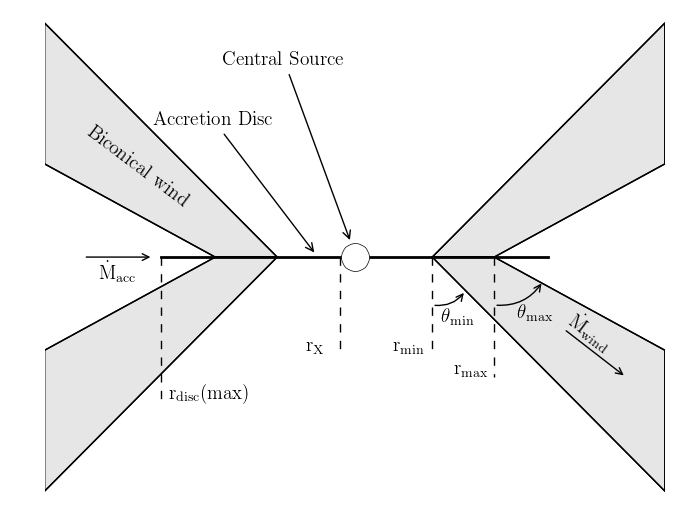
\includegraphics[width=0.45\textwidth]{figures/fig2_cartoon.png}
\caption
{
A cartoon showing the geometry and some key parameters of
our biconical wind model.
}
\label{fig:cartoon}
\end{figure} 

%DIF <  \subsection{A Benchmark Model for BALQSOs}
\DIFdelbegin %DIFDELCMD < 

%DIFDELCMD < %%%
%DIF <  \cite{higginbottom2013} presented a benchmark model for
%DIF <  (BAL)QSOs...introduce key parameters. 
%DIFDELCMD < 

%DIFDELCMD < %%%
\DIFdelend \subsection{Photon Sources}
\DIFaddbegin \label{sec:photon_sources}
\DIFaddend 

%DIF < Describe the photon sources in the model.
\DIFdelbegin %DIFDELCMD < 

%DIFDELCMD < %%%
\DIFdel{The accretion disc }\DIFdelend \DIFaddbegin \DIFadd{We include two sources of r-packets }\DIFaddend in our model\DIFdelbegin \DIFdel{is }\DIFdelend \DIFaddbegin \DIFadd{:
An accretion disc and central X-ray source.
The accretion disc is assumed to be }\DIFaddend geometrically thin, but optically thick.
We thus treat the disc as an ensemble of blackbodies with a 
\cite{shakurasunyaev1973} effective temperature profile. 
The emergent SED is then determined by the specified accretion rate ($\dot{m}$)
and central BH mass ($M_{BH}$).
All photon sources in our model are \DIFdelbegin \DIFdel{assumed to beopaque}\DIFdelend \DIFaddbegin \DIFadd{opaque}\DIFaddend , meaning
that \DIFdelbegin \DIFdel{photons }\DIFdelend \DIFaddbegin \DIFadd{r-packets }\DIFaddend which strike them are destroyed.
The inner radius of the disc extends to the innermost 
stable circular orbit (ISCO) of the BH. 
We assume a Schwarzchild BH with an ISCO at $6~r_G$, where 
$r_G = GM_{BH}/c^2$ is the gravitational radius.
For a $10^9~M_\odot$ black hole, this is equal to $8.8\times10^{14}~{\rm cm}$ 
or $\sim10^{-4}~{\rm pc}$.  


The X-ray source \DIFdelbegin \DIFdel{in our model }\DIFdelend is treated as an isotropic sphere at the ISCO,
which emits r-packets according to a power law in flux with index $\alpha_X$, of the form
\begin{equation}
F_X (\nu) = K\DIFaddbegin \DIFadd{_X }\DIFaddend \nu^{\alpha_X}.
\end{equation}
The normalisation, $K_X$ of this power law is such that it 
produces the specified 2-10~keV luminosity, $L_X$.
In addition to the disc and X-ray source, 
the wind is able to reprocess radiation. However, new 
photon packets are not produced in the wind (as in LK02). 
Instead, this reprocessing is dealt with by enforcing strict
radiative equilibrium ({\em modulo} adiabatic cooling; see section~2.3)
via an indivisible energy packet
constraint (see Lucy 2002, M15).
%DIF <  \begin{equation}

%DIF <  \end{equation}
\DIFdelbegin %DIFDELCMD < 

%DIFDELCMD < %%%
%DIF <  With a normalisation such that it produces the correct 2-10kev luminosity.
%DIFDELCMD < 

%DIFDELCMD < %%%
%DIF <  Photons striking the 
%DIFDELCMD < 

%DIFDELCMD < %%%
%DIF <  which successfully reproduced BAL features 
%DIF <  in synthetic spectra using \py. However, the model
%DIF <  had a few key drawbacks when considering its potential
%DIF <  for unification. First, it failed to produce significant
%DIF <  broad emission lines at non-BAL viewing angles; this is 
%DIF <  a key requirement for a unified QSO model. Second,
%DIF <  the model was significantly X-ray weak, as it was found
%DIF <  that an X-ray luminosity comparable to that of a QSO 
%DIF <  over-ionized the wind, resulting in no UV resonance 
%DIF <  line absorption features.
%DIFDELCMD < 

%DIFDELCMD < %%%
\DIFdelend \subsection{Kinematics and Geometry}

In our model, a biconical disc wind rises from the accretion 
disc between launch radii $r_{min}$ and $r_{max}$.
The opening angles of the wind are set to $\theta_{min}$ and $\theta_{max}$.
The poloidal velocity along each individual streamline at a poloidal distance $l$ 
is then given by
\begin{equation}
v_l=v_0+\left[v_{\infty}(r_0)-v_0\right]\frac{\left(l/R_v\right)^{\alpha}}{\left(l/R_v\right)^{\alpha}+1},
\label{v_law}
\end{equation}
where $v_0$ is the velocity at the base of the streamline, $\alpha$ is
an exponent governing how quickly the wind accelerations and 
$R_v$ is the `acceleration length', defined as the distance at which
the outflow reaches half of its terminal velocity, $v_{\infty}$.
The terminal velocity is set to a fixed multiple of the escape
velocity, $v_{esc}$, at the base of the streamline (radius $r_0$).
The rotational velocity, $v_{\phi}$, is initially Keplerian ($v_k = [GM/r_0]^{1/2}$),
and the wind conserves specific angular momentum, such that 
\begin{equation}
v_{\phi} r = v_k r_0.
\label{v_law}
\end{equation}
The velocity law is crucial in determining the output spectra,
as it affects not only the projected velocities along the line of sight,
but also the density and ionization state of the outflow.
A wind \DIFdelbegin \DIFdel{which }\DIFdelend \DIFaddbegin \DIFadd{that }\DIFaddend accelerates more slowly will have a denser wind base
with correspondingly different ionization and emission characteristics.

\subsection{\DIFaddbegin \DIFadd{A First Approximation for }\DIFaddend Clumping}

\DIFaddbegin \DIFadd{Our previous modelling efforts assumed a smooth outflow, 
in which the density at a given point was determined only by the 
kinematic parameters and mass loss rate. However, as already discussed,
AGN winds exhibit significant substructure -- the outflow is expected to be
}{\em \DIFadd{clumpy}}\DIFadd{, rather than smooth, and probably on a variety of scales. 
Implementing a treatment of clumping is challenging, for
two main reasons. First, there are significant 
computational difficulties associated with adequately
resolving and realistically modelling a series of small scale, high density
regions with a MCRT code. Second, the addition of multiple additional degrees of
freedom in the model results in significantly wider parameter space.
Unfortunately, the physical scale lengths and density contrasts 
associated with these parameters cannot be well-constrained from observations.
}

\DIFaddend To allow for clumping in our outflow we adopt a simple approximation
used \DIFdelbegin \DIFdel{extensively }\DIFdelend \DIFaddbegin \DIFadd{successfully }\DIFaddend in stellar wind modelling, known as 
{\em microclumping} \DIFdelbegin \DIFdel{\mbox{%DIFAUXCMD
\citep{hamann1998}
}%DIFAUXCMD
}\DIFdelend \DIFaddbegin \DIFadd{\mbox{%DIFAUXCMD
\citep{hamann1998,hamann2008}
}%DIFAUXCMD
(MORE REFS)}\DIFaddend . 
The key assumption \DIFdelbegin \DIFdel{here }\DIFdelend is that typical clump sizes are much smaller than the 
typical photon mean free path, and thus the clumps are 
both geometrically and optically thin. This approach 
allows one to introduce a `\DIFaddbegin \DIFadd{volume }\DIFaddend filling factor', \DIFdelbegin \DIFdel{$f$, which is the 
fraction of the volume of the plasma filled by clumps}\DIFdelend \DIFaddbegin \DIFadd{$f_V$}\DIFaddend . 
The intra-clump medium is assumed to be a vacuum\DIFdelbegin \DIFdel{. We can then introduce the density enhancement, $D$, which is defined as 
}\begin{displaymath}\DIFdel{
D = \frac{1}{f}.
}\end{displaymath}
%DIFAUXCMD
\DIFdel{We then multiply all densities in the model by }\DIFdelend \DIFaddbegin \DIFadd{, so the 
density of the clumps is then multiplied by the ``density enhancement'' 
$D=1/f_V$. Opacities, $\kappa$, and emissivities, $\epsilon$, 
can then be expressed as 
}

%DIF >  \begin{subequations}
%DIF >  \begin{align}
%DIF >          \kappa &= f_V \kappa_C(D) \\
%DIF >          \epsilon &= f_V \epsilon_C(D)
%DIF >  \end{align}
%DIF >  \end{subequations}
\begin{equation}\DIFadd{
\kappa = f_V \kappa_C(D);~~\epsilon = f_V \epsilon_C(D).
}\end{equation}
%DIF >  \kappa = f_V \kappa_C(D) && \epsilon = f_V \epsilon_C(D).
%DIF >  \end{equation}
\DIFadd{Here the subscript $C$ denotes that the quantity is calculated using the 
enhanced density in the clump. The resultant effect is that }{\em \DIFadd{linear}} \DIFadd{processes,
such as electron scattering, are unchanged, as $f_V$ and }\DIFaddend $D$ \DIFdelbegin \DIFdel{, and all emitting volumes
by $f$. This has the effect of enhancing all emissivities and opacities
that scale with the square of density (}\DIFdelend \DIFaddbegin \DIFadd{will cancel out. 
However, any quantity which scales with the }{\em \DIFadd{square}} \DIFadd{of density, 
}\DIFaddend such as collisional excitation \DIFdelbegin \DIFdel{and recombination) 
}\DIFdelend \DIFaddbegin \DIFadd{or recombination, will increase }\DIFaddend by a factor \DIFaddbegin \DIFadd{of }\DIFaddend $D$.
\DIFdelbegin \DIFdel{All processes that scale linearly with density 
(such as electron scattering and bound-free opacity)
will remain unchanged for a given ionization state. 
%DIF <  A factor $f$ is also
%DIF <  applied to the opacities such that opacities which scale only with $\rho$ are not
%DIF <  increased. 
}\DIFdelend 

%DIF >  which is defined as 
%DIF >  \begin{equation}
%DIF >  D = \frac{1}{f} && 
%DIF >  \end{equation}
%DIF >  We then multiply all densities in the model by $D$, and all emitting volumes
%DIF >  by $f$. This has the effect of enhancing all emissivities and opacities
%DIF >  that scale with the square of density (such as collisional excitation and recombination) 
%DIF >  by a factor $D$. All processes that scale linearly with density 
%DIF >  (such as electron scattering and bound-free opacity)
%DIF >  will remain unchanged for a given ionization state. 
\DIFaddbegin 

\DIFaddend Clumping the wind has an important effect on the ionization state and has
been proposed as a solution to the so-called `over-ionization problem' in 
disc winds \DIFdelbegin \DIFdel{(REFs)}\DIFdelend \DIFaddbegin \DIFadd{\mbox{%DIFAUXCMD
\citep{hamann2013}
}%DIFAUXCMD
}\DIFaddend . This is the main motivation for incorporating microclumping
into our model. This treatment is first-order; it does not adequately
represent the complex substructures and stratifications in ionization
state we expect in AGN outflows. Nevertheless, clumping is clearly
important in these flows, and this parameterization allows a simple estimate
for the effect clumping might have on the ionization state and emergent 
line emission. 
\DIFdelbegin \DIFdel{It is also encouraging that microclumping has been used 
successfully in fits to O-star wind spectra \mbox{%DIFAUXCMD
\citep{hillier1991eswingsmodel}
}%DIFAUXCMD
.
}\DIFdelend %DIF >  It is also encouraging that microclumping has been used 
%DIF >  successfully in fits to O-star wind spectra \citep{hillier1991eswingsmodel}.

%DIF < %%%%%%%%%%%%%%%%%%%%%%%%%%%%%%%%%%%%%%%%%%%%%%%%
\DIFaddbegin \subsection{\DIFadd{The Simulation Grid: Arriving at a next-generation model}}
\DIFaddend 

%DIF <  RESULTS
\DIFdelbegin %DIFDELCMD < 

%DIFDELCMD < %%%
%DIF < %%%%%%%%%%%%%%%%%%%%%%%%%%%%%%%%%%%%%%%%%%%%%%%%
%DIFDELCMD < 

%DIFDELCMD < %%%
\section{\DIFdel{Results and Discussion}}
%DIFAUXCMD
\addtocounter{section}{-1}%DIFAUXCMD
%DIFDELCMD < 

%DIFDELCMD < %%%
\DIFdel{Here we describe the results from our model, the parameters
of which are shown in table~1.
Parameters differing from the benchmark model of
H13 are highlighted with an asterisk.
This set of parameters
was arrived at by conducting a limited grid }\DIFdelend \DIFaddbegin \DIFadd{Using this prescription, we conducted a limited parameter
}\DIFaddend search over a 5-dimensional parameter space involving the 
variables $r_{min}$, $\theta_{min}$, \DIFdelbegin \DIFdel{$f$}\DIFdelend \DIFaddbegin \DIFadd{$f_V$}\DIFaddend , $\alpha$ and \DIFdelbegin \DIFdel{$R_V$.
The full grid , including output spectral files and plots can be found at
}%DIFDELCMD < \url{jhmatthews.github.io/quasar-wind-grid/}%%%
\DIFdel{. 
We }\DIFdelend \DIFaddbegin \DIFadd{$R_v$.
The grid points are shown in table 1.
The aim here was to first fix $M_{BH}$ and $\dot{m}$ to their H13 values,
and increase $L_X$ to $10^{45}$~erg~s$^{-1}$ (a more realistic value for a 
quasar of $10^9M_\odot$ and an eddington fraction of $0.2$; see section~\ref{sec:xray}). 
We then }\DIFaddend evaluated these models \DIFdelbegin \DIFdel{qualitatively }\DIFdelend based on the following criteria:
\begin{itemize}
\item Does the model \DIFdelbegin \DIFdel{maintain the right ionization state to produce strong BALs}\DIFdelend \DIFaddbegin \DIFadd{avoid over-ionization and thus produce UV absorption lines 
with $BI > 0$ at $\sim20\%$ of viewing angles}\DIFaddend ?
\item Does significant line emission emerge at low inclinations\DIFaddbegin \DIFadd{, with $EW\sim40\AA$ in }\civ\DIFaddend ?
\item Do H recombination lines appear in the spectrum\DIFaddbegin \DIFadd{, $EW\sim50\AA$ in }\la\DIFaddend ?
\item Do a \DIFdelbegin \DIFdel{certain range of }\DIFdelend \DIFaddbegin \DIFadd{small subset of BAL }\DIFaddend angles produce LoBAL features?
\item Does the model compare favourably to quasar composite spectra?
\end{itemize}
In this section, we present one of the most promising models and discuss
the various successes and failures \DIFaddbegin \DIFadd{with respect to the above criteria}\DIFaddend .
This allows us to gain insight into fundamental geometrical 
and physical constraints and assess the potential for unification. 
\DIFdelbegin %DIFDELCMD < 

%DIFDELCMD < \begin{figure*} %%%
%DIF < fullpage
%DIFDELCMD < \centering
%DIFDELCMD < 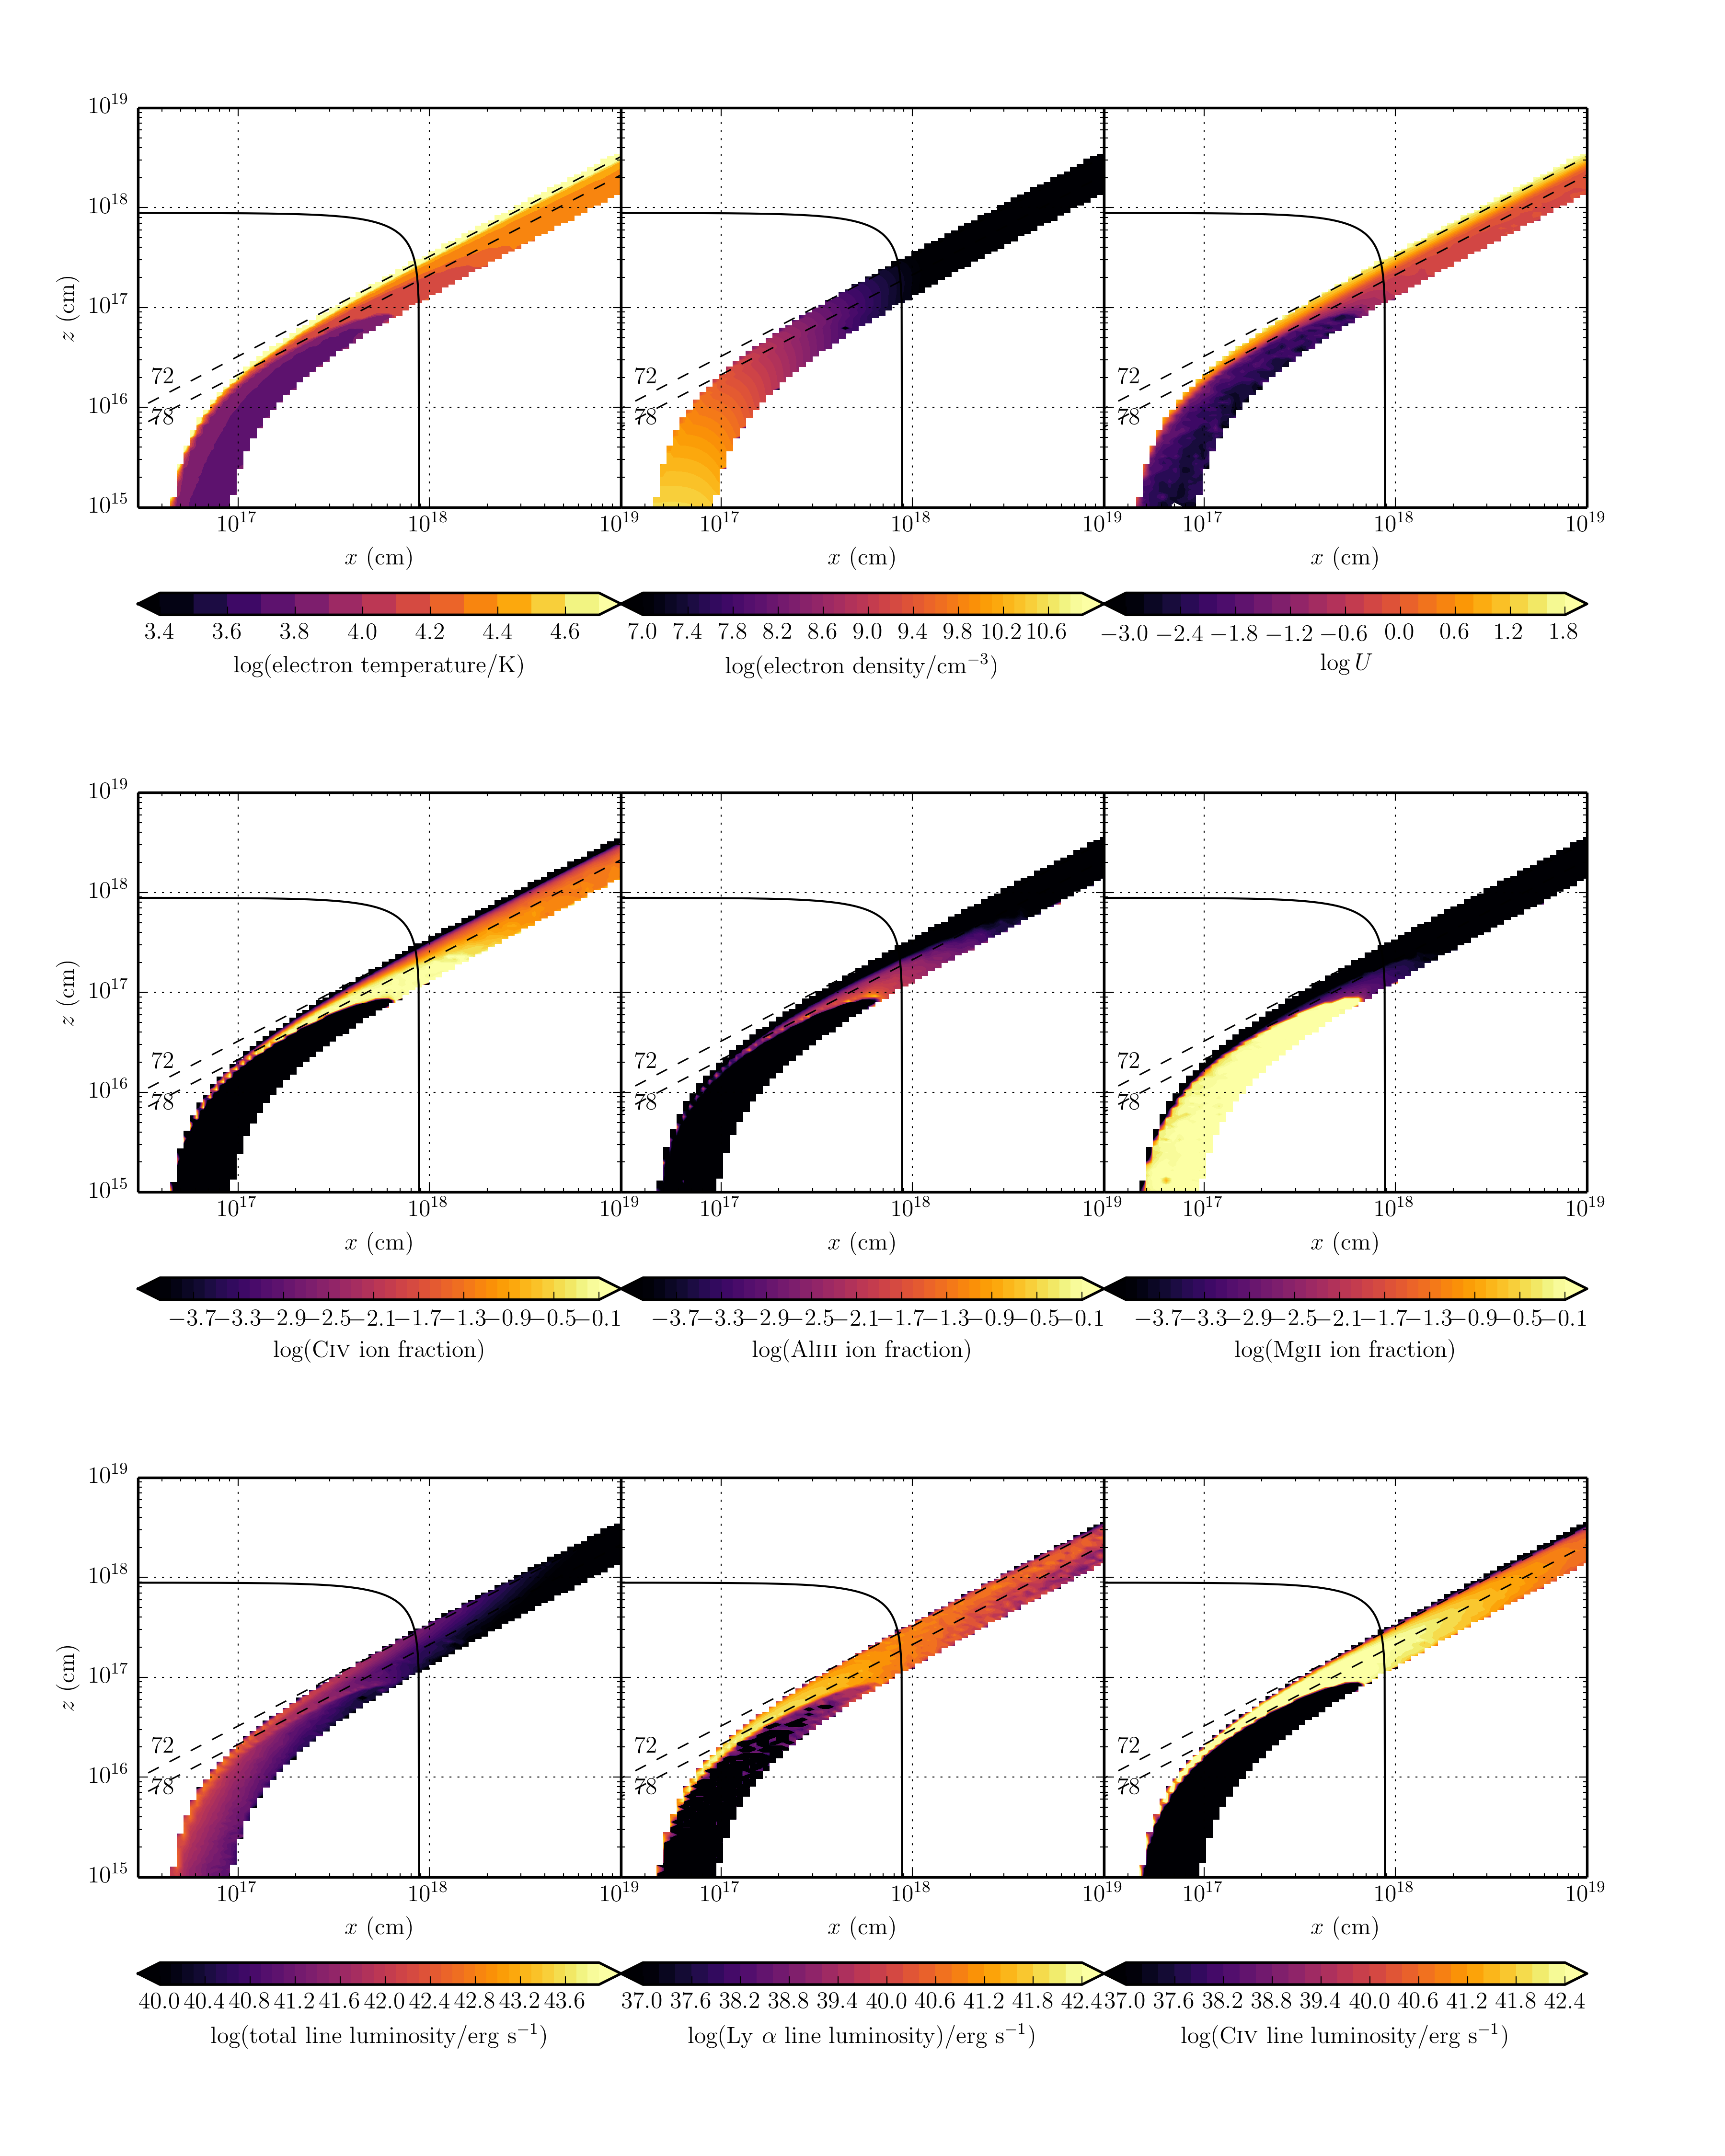
\includegraphics[width=1.0\textwidth]{figures/link.png}
%DIFDELCMD < \caption
%DIFDELCMD < {
%DIFDELCMD < %%%
\DIFdel{Physical properties of the outflow,
shown by the coloured contours. The solid black line marks a sphere at $1000~r_G$. The dotted lines show the $72^\circ$ and $78^\circ$ sightlines 
to the centre of the system, 
and illustrate that different sightlines
intersect material of different ionization states }\DIFdelend \DIFaddbegin \DIFadd{The full grid, including output synthetic spectra and plots can be found at
}\url{jhmatthews.github.io/quasar-wind-grid/}\DIFaddend .
\DIFdelbegin %DIFDELCMD < }
%DIFDELCMD < \label{fig:wind}
%DIFDELCMD < \end{figure*} %%%
%DIF < fullpage
\DIFdelend 

\begin{table}
\DIFaddbeginFL \begin{tabular}{p{2cm}p{1cm}p{1cm}p{1cm}p{1cm}}
\DIFaddFL{Parameter }& \multicolumn{4}{|l|}{Grid Point Values}  \\
\hline \hline 
\DIFaddFL{$r_{min}$ 	}&	 \DIFaddFL{$6r_{g}$ }& \DIFaddFL{$60r_{g}$ }& \multicolumn{2}{|l|}{$300r_{g}$} \\ 
\DIFaddFL{$\theta_{min}$ 	}&	 \DIFaddFL{$40^{\circ}$ }& \DIFaddFL{$55^{\circ}$ }& \multicolumn{2}{|l|}{$70^{\circ}$} \\ 
\DIFaddFL{$R_v$  	        }&	 \DIFaddFL{$10^{18}$cm }& \multicolumn{3}{|l|}{$10^{19}$cm} \\ 
\DIFaddFL{$\alpha$ 	}&	 \DIFaddFL{$0.5$ }& \DIFaddFL{$0.6$ }& \DIFaddFL{$0.75$ }& \DIFaddFL{$1.5$ }\\
\DIFaddFL{$f_V$ 	}&	 \DIFaddFL{$0.01$ }& \DIFaddFL{$0.1$ }& \multicolumn{2}{|l|}{$1$}  \\
\hline 
\end{tabular}
\caption{\DIFaddFL{The grid points used in the parameter search.}}
\label{grid_table}
\end{table}



%DIF > %%%%%%%%%%%%%%%%%%%%%%%%%%%%%%%%%%%%%%%%%%%%%%%%

%DIF >  RESULTS

%DIF > %%%%%%%%%%%%%%%%%%%%%%%%%%%%%%%%%%%%%%%%%%%%%%%%


\section{\DIFadd{Results and Discussion}}

%DIF >  {\bf We need to describe what we did before getting to results.  We started with parameters similar to those of H14, we created a small grid.  Limits of the grid are given in table 2.  This should be a paragraph or section before this one.  Not all quasars have to have the same parameters and so we have to explain that we have elected to describe one model in detail.  Was our goal to fix the luminosity and see what was required.

%DIF >  In next sections, we really need to deal with the difference between this class of models and "the model", and especially "our model".  We may need to at least in words discuss whether we have "fine tuned" or not, by saying something about other models.}

\DIFadd{Here we describe the results from our next-generation model,
and discuss these results in the context of the criteria 
presented in section 3.4. The parameters of this model are shown in table~2.
Parameters differing from the benchmark model of H13 are 
highlighted with an asterisk. In this section, we examine the physical 
conditions of the flow, and present the synthetic spectra, before comparing
the X-ray properties of this particular model to samples of
quasars and luminous AGN. We also examine trends with inclination in the synthetic spectra, 
both in terms of the range of ionization states of the absorption lines and equivalent widths 
of the emission lines.
}

%DIF >  This set of parameters
%DIF >  was arrived at by conducting a limited grid search over a 
%DIF >  5-dimensional parameter space involving the variables
%DIF >  $r_{min}$, $\theta_{min}$, $f$, $\alpha$ and $R_V$.
%DIF >  We evaluated these models based on the following
%DIF >  criteria:
%DIF >  \begin{itemize}
%DIF >  \item Does the model maintain the right ionization state to produce strong BALs ($BI > ??$)?
%DIF >  \item Does significant line emission emerge at low inclinations, with $EW\sim50\AA$ in \civ?
%DIF >  \item Do H recombination lines appear in the spectrum, $EW\sim50\AA$ in \la?
%DIF >  \item Do a certain range of angles produce LoBAL features?
%DIF >  \item Does the model compare favourably to quasar composite spectra?
%DIF >  \end{itemize}
%DIF >  In this section, we present one of the most promising models and discuss
%DIF >  the various successes and failures.
%DIF >  This allows us to gain insight into fundamental geometrical 
%DIF >  and physical constraints and assess the potential for unification. 
%DIF >  The full grid, including output synthetic spectra and plots can be found at
%DIF >  \url{jhmatthews.github.io/quasar-wind-grid/}.



\begin{table}
\DIFaddendFL \begin{tabular}{p{3cm}p{4cm}}
\hline \DIFdelbeginFL \DIFdelFL{Free }\DIFdelendFL \DIFaddbeginFL \DIFaddFL{Next-generation Model }\DIFaddendFL Parameters 	&	 Value \\ 
\hline \hline 
$M_{BH}$ 	 &	 $1\times 10^9~\rm{M_{\odot}}$ \\ 
$\dot{M}_{acc}$ 	 &	 $5~M_{\odot}yr^{-1} \simeq 0.2~\dot{M}_{Edd}$\\ 
$\alpha_X$ 	 &	 $-0.9$ \\ 
$L_{X} $ 	 &	 $10^{45}~\rm{ergs~s^{-1}}$$^*$ \\ 
$r_{disc}(min)=r_{X}$   &	 $6r_g=8.8\times10^{14}~{\rm cm}$ \\ 
$r_{disc}(max)$   &	 $3400r_g = 5\times10^{17}~{\rm cm}$ \\ 
$\dot{M}_{wind}$  &	 $5~M_{\odot}yr^{-1}$ \\ 
$r_{min}$ 	&	 $300r_{g} = 4.4\times10^{16}~{\rm cm}$\\ 
$r_{max}$ 	&	 $600r_{g} = 8.8\times10^{16}~{\rm cm}$ \\ 
$\theta_{min}$ 	&	 $70.0^{\circ}$ \\ 
$\theta_{max}$ 	&	 $82.0^{\circ}$ \\ 
$\lambda$ 	&	 $0$ \\ 
$v_{\infty}(r_0)$ 	&	 $v_{esc}(r_0)$ \\ 
$R_v$  	        &	 $10^{19}$cm$^*$ \\ 
$\alpha$ 	&	 $0.6^*$ \\
\DIFdelbeginFL \DIFdelFL{$f$ 	}\DIFdelendFL \DIFaddbeginFL \DIFaddFL{$f_V$ 	}\DIFaddendFL &	 $0.01^*$  \\
\DIFaddbeginFL \DIFaddFL{$n_x$ 	}&	 \DIFaddFL{$100$  }\\
\DIFaddFL{$n_z$ 	}&	 \DIFaddFL{$200$  }\\
\DIFaddendFL \hline 
% Derived Parameters 	&	 Value \\ 
% \hline \hline
% $L_{\nu}(2500\mbox{\scriptsize{\AA}})$&	 $6.3\times10^{30}~\rm{ergs~s^{-1}~Hz^{-1}}$\\ 
% $L_{\nu}(2keV)$   &	 $1.2\times10^{25}~\rm{ergs~s^{-1}~Hz^{-1}}$\\ 
% $L_{bol}$ 	 &	 $2.4\times10^{46}~\rm{ergs~s^{-1}}$\\
% $M_{bol}$ 	 &	 -27.4\\ 
% $M_u$            &	 -26.2\\ 
% $\alpha_{OX} $ 	 &	 -2.2\\ 
\end{tabular}
\caption{Wind geometry parameters used in the model.}
\label{wind_param}
\end{table}



\subsection{Physical Conditions and Ionization State}


\DIFaddbegin \begin{figure*} %DIF > fullpage
\centering
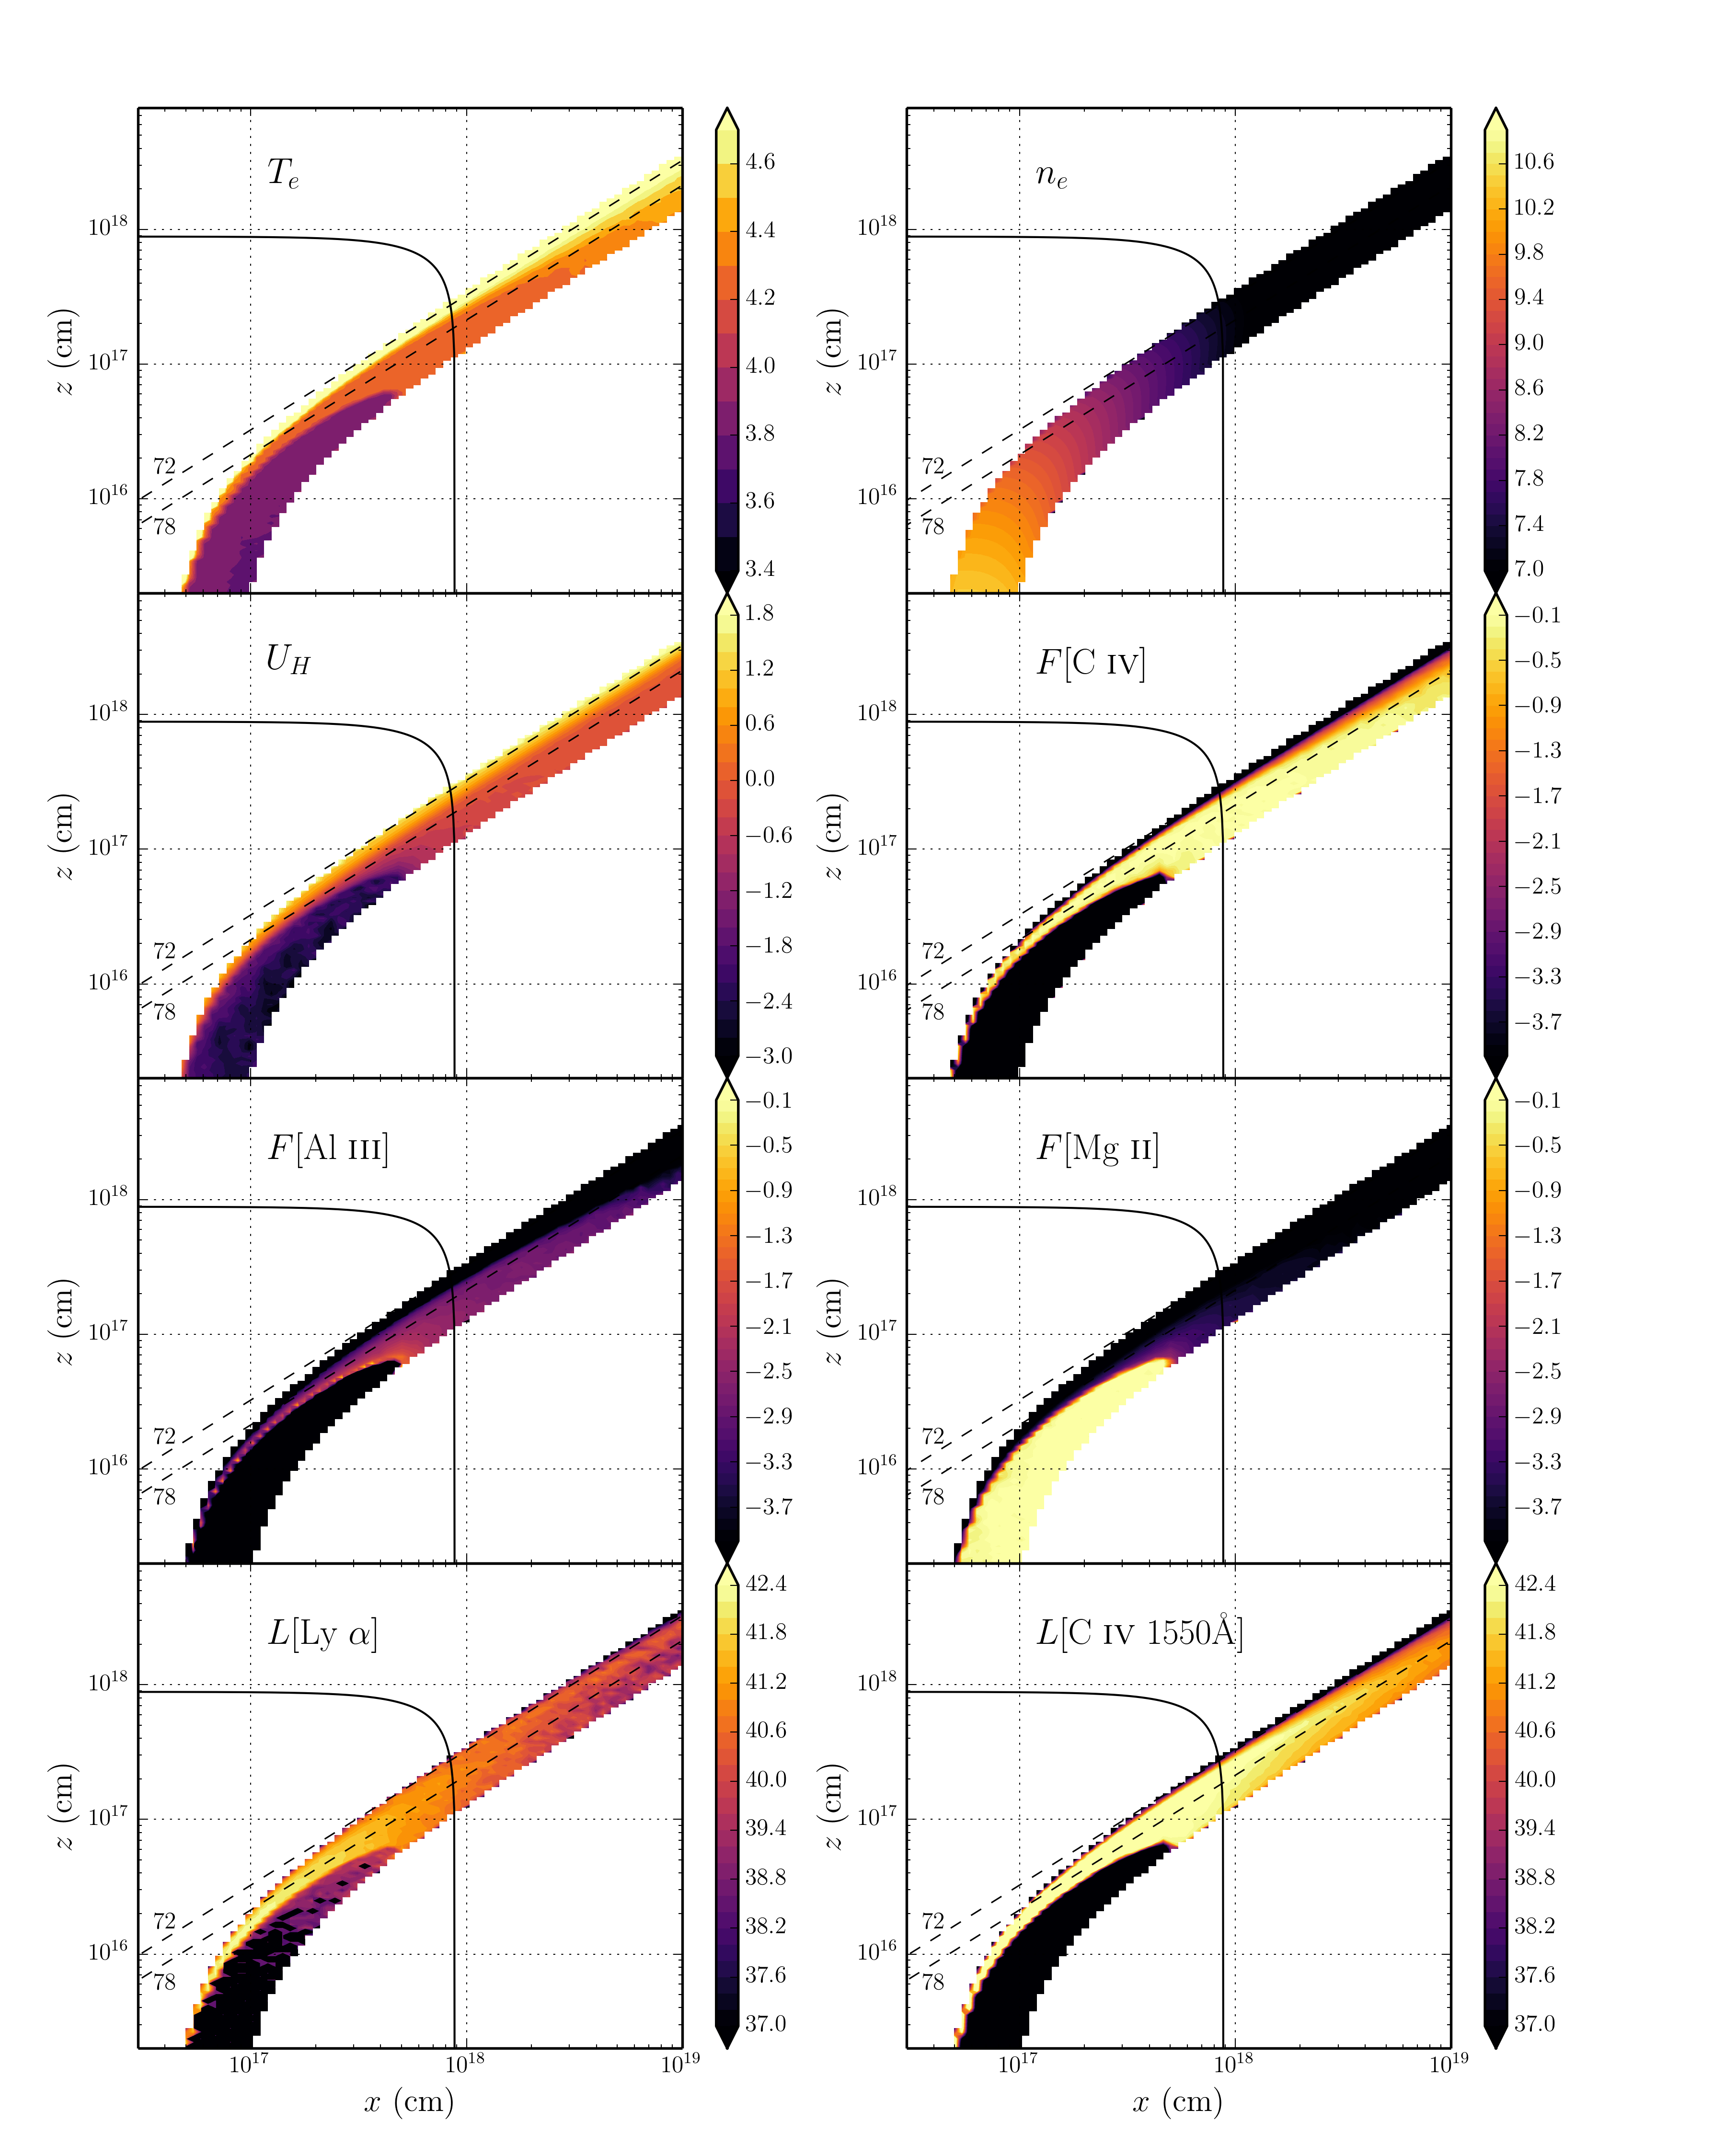
\includegraphics[width=1.0\textwidth]{figures/link8.png}
\caption
{
\DIFaddFL{Contour plots showing the logarithm of some important 
physical properties of the outflow. Symbols are defined in the text.
The solid black line marks a sphere at $1000~r_G$.
The dotted lines show the $72^\circ$ and $78^\circ$ sightlines 
to the centre of the system, and illustrate that different sightlines
intersect material of different ionization states.
The line luminosities represent the luminosity of photons
escaping the Sobolev region for each line. These photons do not
necessarily escape to infinity.
}}
\label{fig:wind}
\end{figure*} %DIF > fullpage

\DIFaddend Figure~\ref{fig:wind} shows the physical properties of the wind.
The wind rises slowly from the disc at first, with clumped densities
of $n_H \sim 10^{11}~\rm{cm^{-3}}$ close to the disc plane.
The flow then accelerates over a scale length of $R_V=10^{19}~\rm{cm}$
up to a terminal velocity equal to the escape velocity at the streamline base
($\sim10,000~\rm{km~s^{-1}}$). This gradual acceleration means that
the wind exhibits a stratified ionization structure, with low ionization material
in the base of the wind giving way to highly ionized plasma further out.
\DIFaddbegin \DIFadd{This is illustrated in figure~\ref{fig:wind} 
by the panels showing the ion fraction $F=n_j/n_{tot}$ of some important ions.
}\DIFaddend By clumping the wind, we are able to produce the range of ionization states observed
in quasars and BALQSOs, while adopting a realistic $2-10$ keV X-ray luminosity
of $L_{X}=10^{45}~\rm{ergs~s^{-1}}$. Without clumping, this wind would be over-ionized 
to the extent that opacities in e.g., \civ\ would be entirely negligible (see H13).

One common way to quantify the ionization state of a plasma
is through the ionization parameter, $U_H$, given by
\begin{equation}
U_H = \frac{4\pi}{n_H c}\int_{13.6{\rm{eV}}}^{\infty}\frac{{J_{\nu}d\nu}}{h\nu}.
\end{equation}
\noindent where $\rm{n_H}$ is the local number density of H, and $\nu$ denotes photon 
frequency. Shown in figure~\ref{fig:wind},
the ionization parameter is a useful measure of the global ionization state,
as it represents the ratio of the number density of 
H ionizing photons to the local H density.
It is, however, a poor representation of the 
ionization state of species such as \civ\ as it encodes no information
about the shape of the SED. In our case, the X-ray photons 
are dominant in the photoionization of the UV resonance line ions. 
This explains why a factor of 100 increase in X-ray luminosity requires
a clumping factor of 0.01, even though the value of $U_H$ decreases by only a factor of $\sim10$ 
compared to H13. 
\DIFdelbegin \DIFdel{This is also the reason for significant Lyman edge photoabsorption
at the highest inclinations (see section 4.3).
}\DIFdelend %DIF > This is also the reason for significant Lyman edge photoabsorption
%DIF > at the highest inclinations (see section 4.3).

Clumping also causes the total line luminosity to increase dramatically,
as recombination and collisional excitation are both proportional to
\DIFdelbegin \DIFdel{$n_e^2$}\DIFdelend \DIFaddbegin \DIFadd{density squared}\DIFaddend . This line emission typically emerges on the edge of the wind
nearest the central source. The location of the line emitting regions
is dependent on the ionization state, as well as the X-rays heating the plasma.
The radii of these emitting regions is important,
and can be compared to observations. \DIFaddbegin \DIFadd{The line luminosities 
shown in the figure correspond to the luminosity in $\LUM$ of photons
escaping the Sobolev region for each line. 
This is equivalent to $\beta_{ul} n_u A_{ul}$, where the three quantities
represent the Sobolev escape probability, upper level number density and 
Einstein A coefficient for the line. 
}\DIFaddend As shown in figure~\ref{fig:wind},
the \civ\ line in our model is typically formed between 
$100-1000~r_G$ ($\sim10^{17}-10^{18}~\rm{cm}$).
This is in rough agreement with the reverberation mapping 
results of Kaspi (2000) for the $2.6\times10^{9} M_\odot$ quasar S5 0836+71,
and also compares favourably with microlensing measurements of the size of the
\civ\ emission line region in the BALQSO H1413+117 \citep{odowd2015}.


\subsection{Synthetic Spectra\DIFaddbegin \DIFadd{: Comparison to Observations}\DIFaddend }

\begin{figure*} %fullpage
\centering
\DIFdelbeginFL %DIFDELCMD < 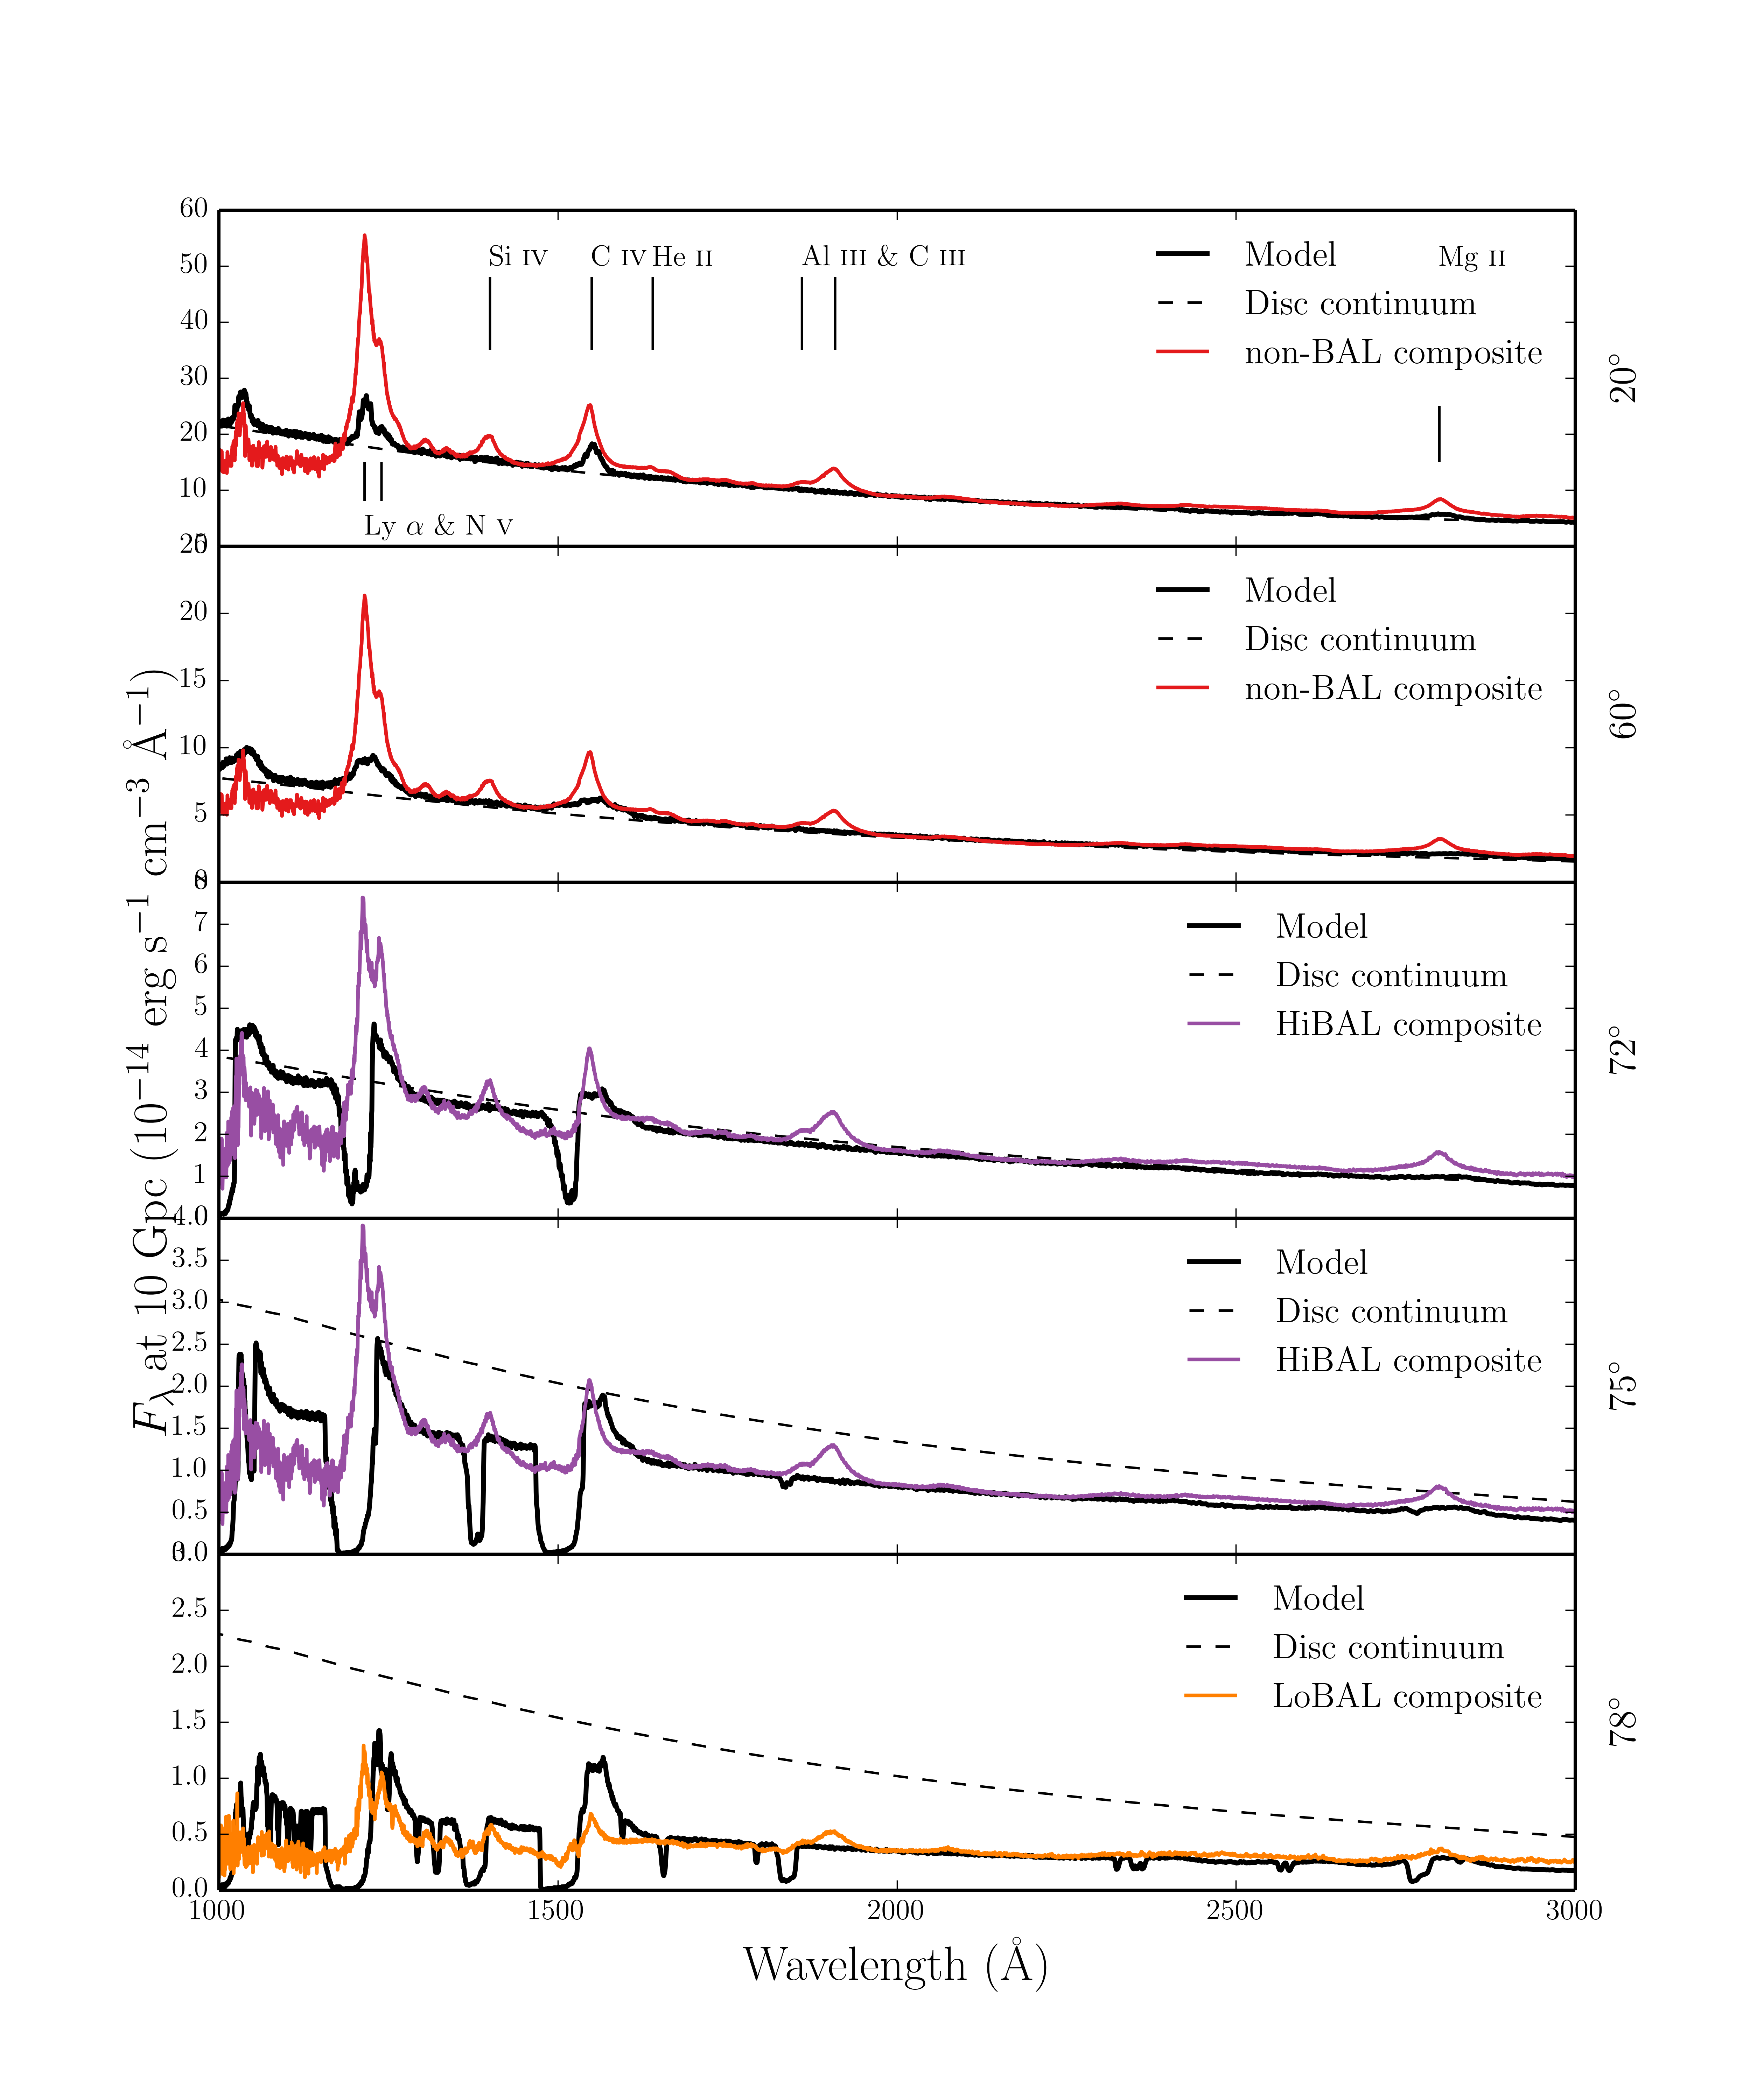
\includegraphics[width=1.0\textwidth]{figures/uvspec.png}
%DIFDELCMD < %%%
\DIFdelendFL \DIFaddbeginFL 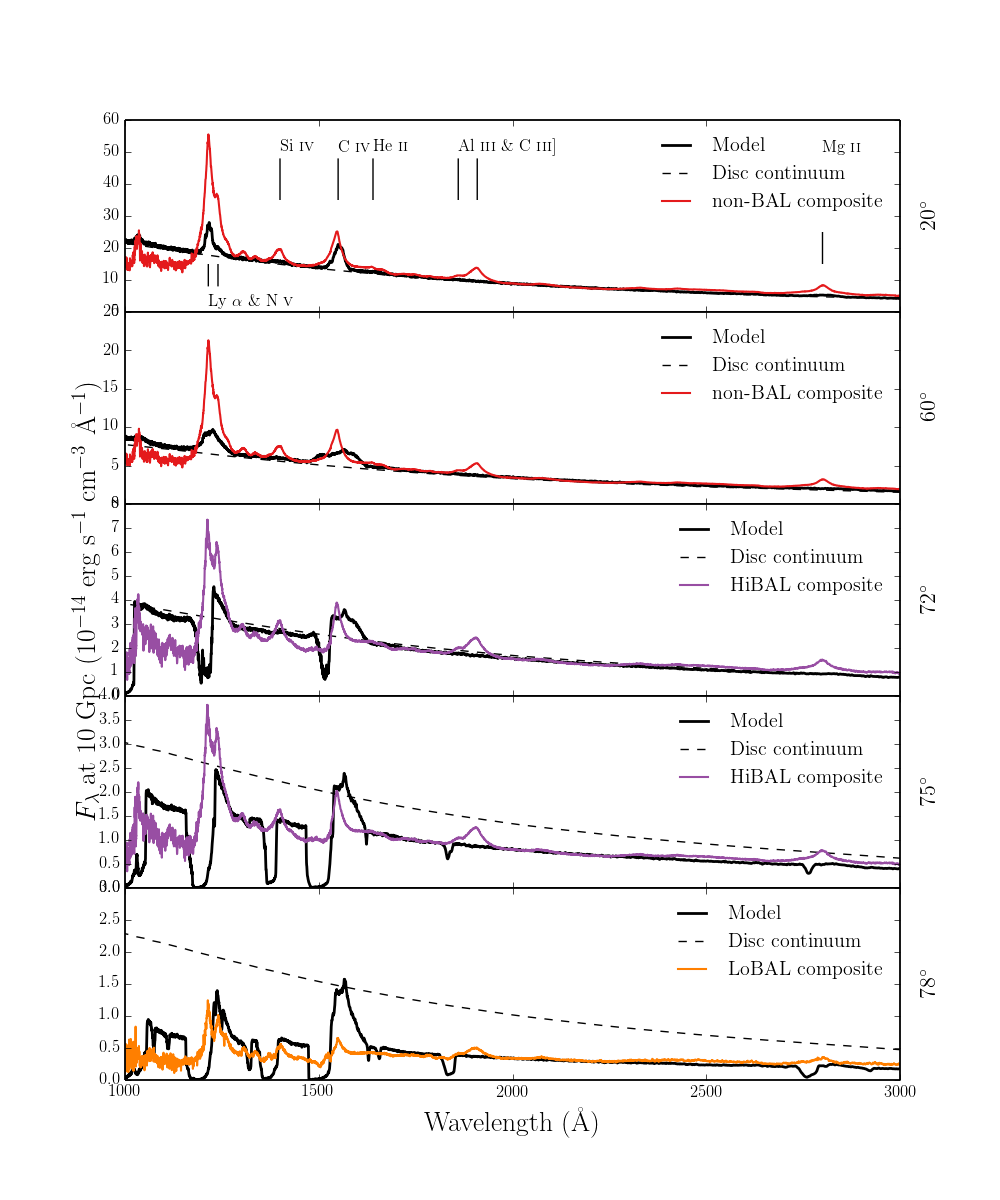
\includegraphics[width=1.0\textwidth]{figures/uvspec_estfix.png}
\DIFaddendFL \caption
{
Synthetic spectra at five viewing angles in our model. The coloured lines
show different quasar and BAL quasar composites, and the dotted line shows a disc
only continuum to show the effect of the outflow on the continuum level.  
}
\label{fig:uvspec}
\end{figure*} %fullpage

\begin{figure} 
\centering
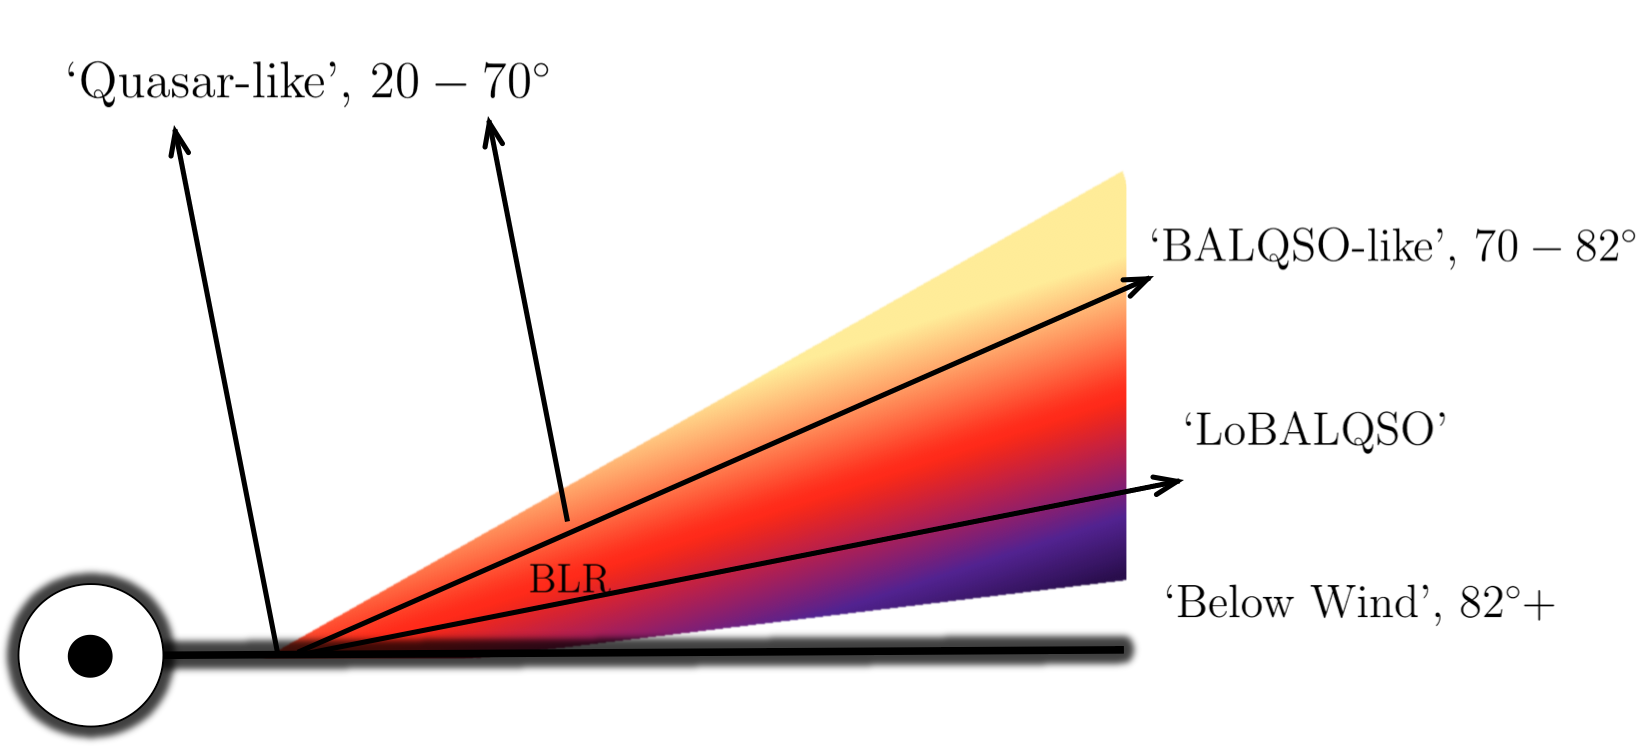
\includegraphics[width=0.5\textwidth]{figures/windnew3.png}
\caption
{
A cartoon describing the broad classes of sightline 
in our model, illustrating how geometric effects lead to 
the different emergent spectra. The colour gradient is approximate,
but indicates the stratified ionization structure, 
from highly ionized (yellow) to low ionization (purple) material.
%[FIGURE NEEDS IMPROVING]
}
\label{fig:sightline}
\end{figure} 

%DIF <  \begin{figure*} %fullpage
%DIF <  \centering
%DIF <  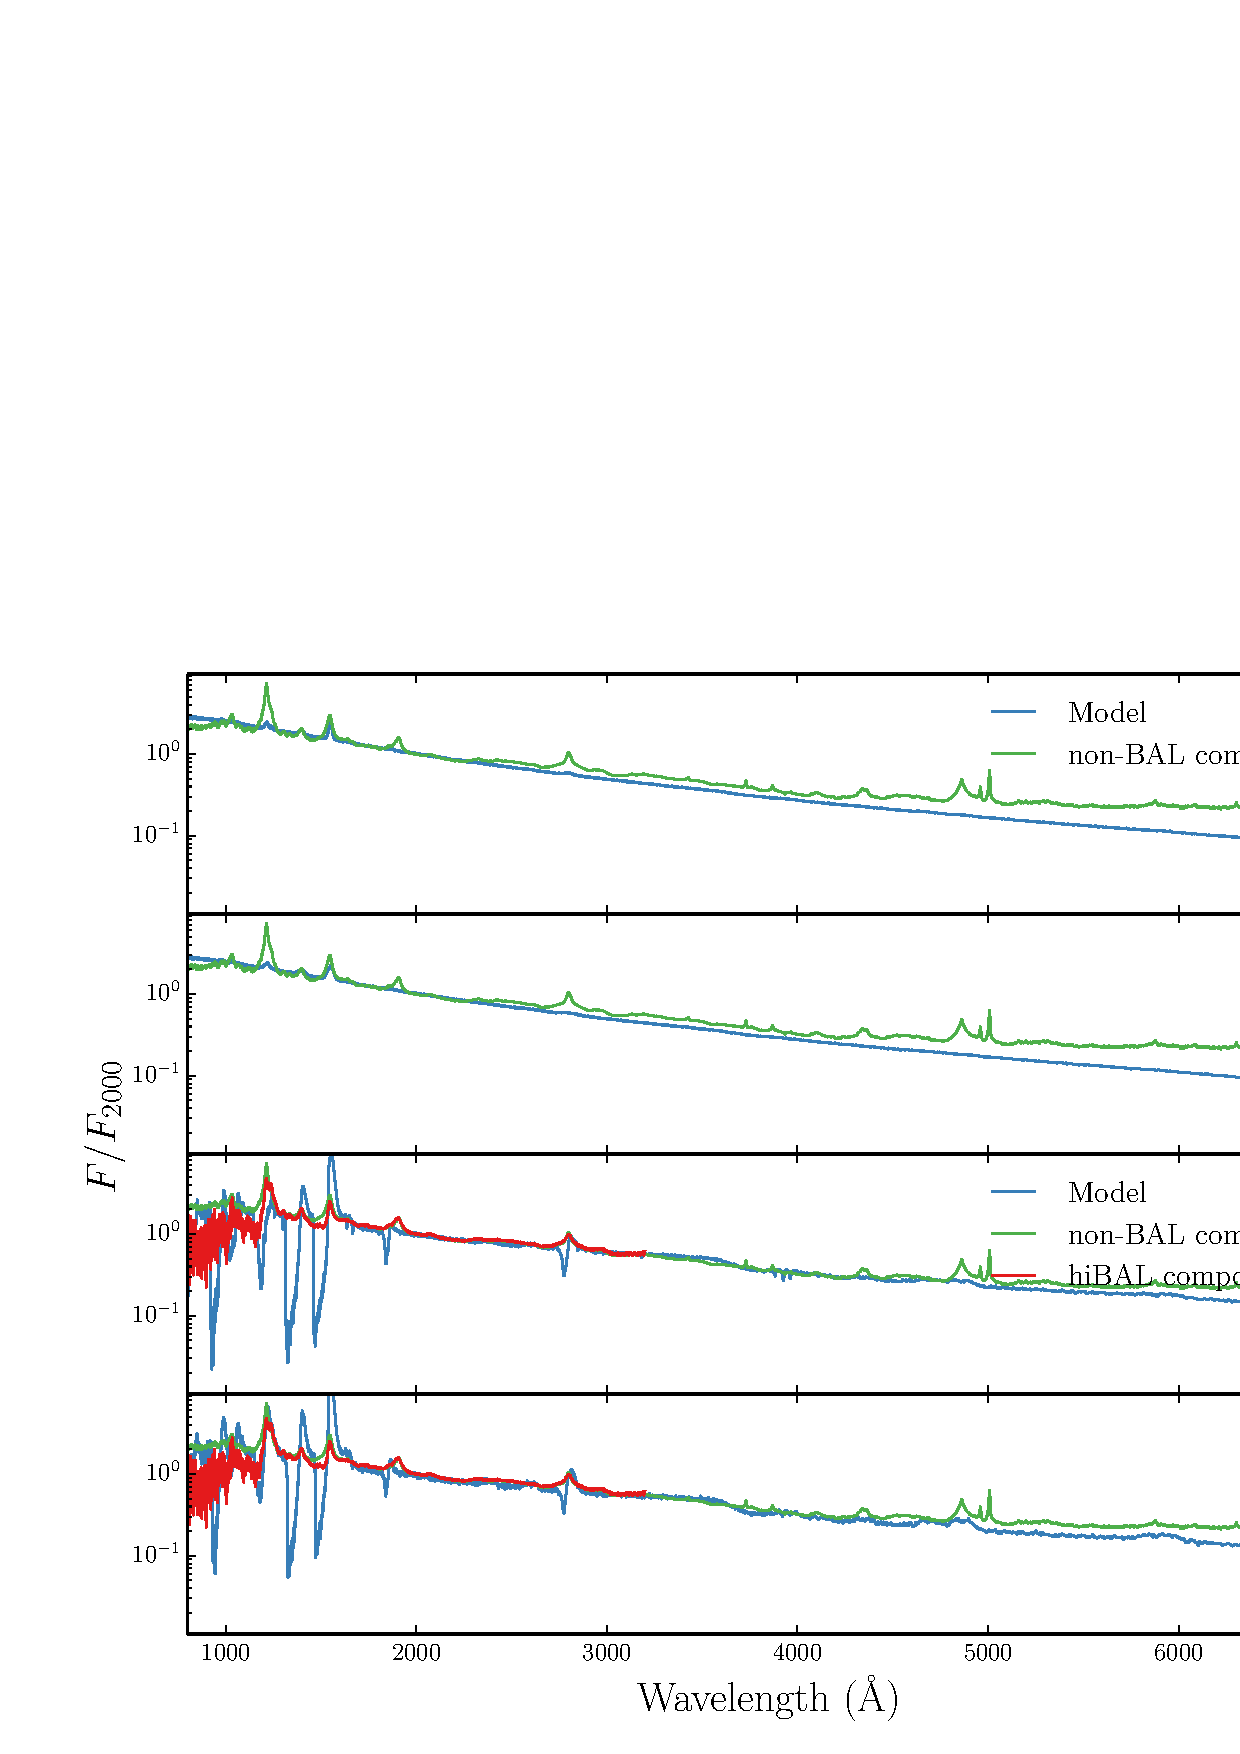
\includegraphics[width=1.0\textwidth]{figures/opt.png}
%DIF <  \caption
%DIF <  {
%DIF <  Figure designed to show optical spectrum and comparison to composite.
%DIF <  }
%DIF <  \label{fig:uvspec}
%DIF <  \end{figure*} %fullpage
\DIFaddbegin \begin{figure*} %DIF > fullpage
\centering
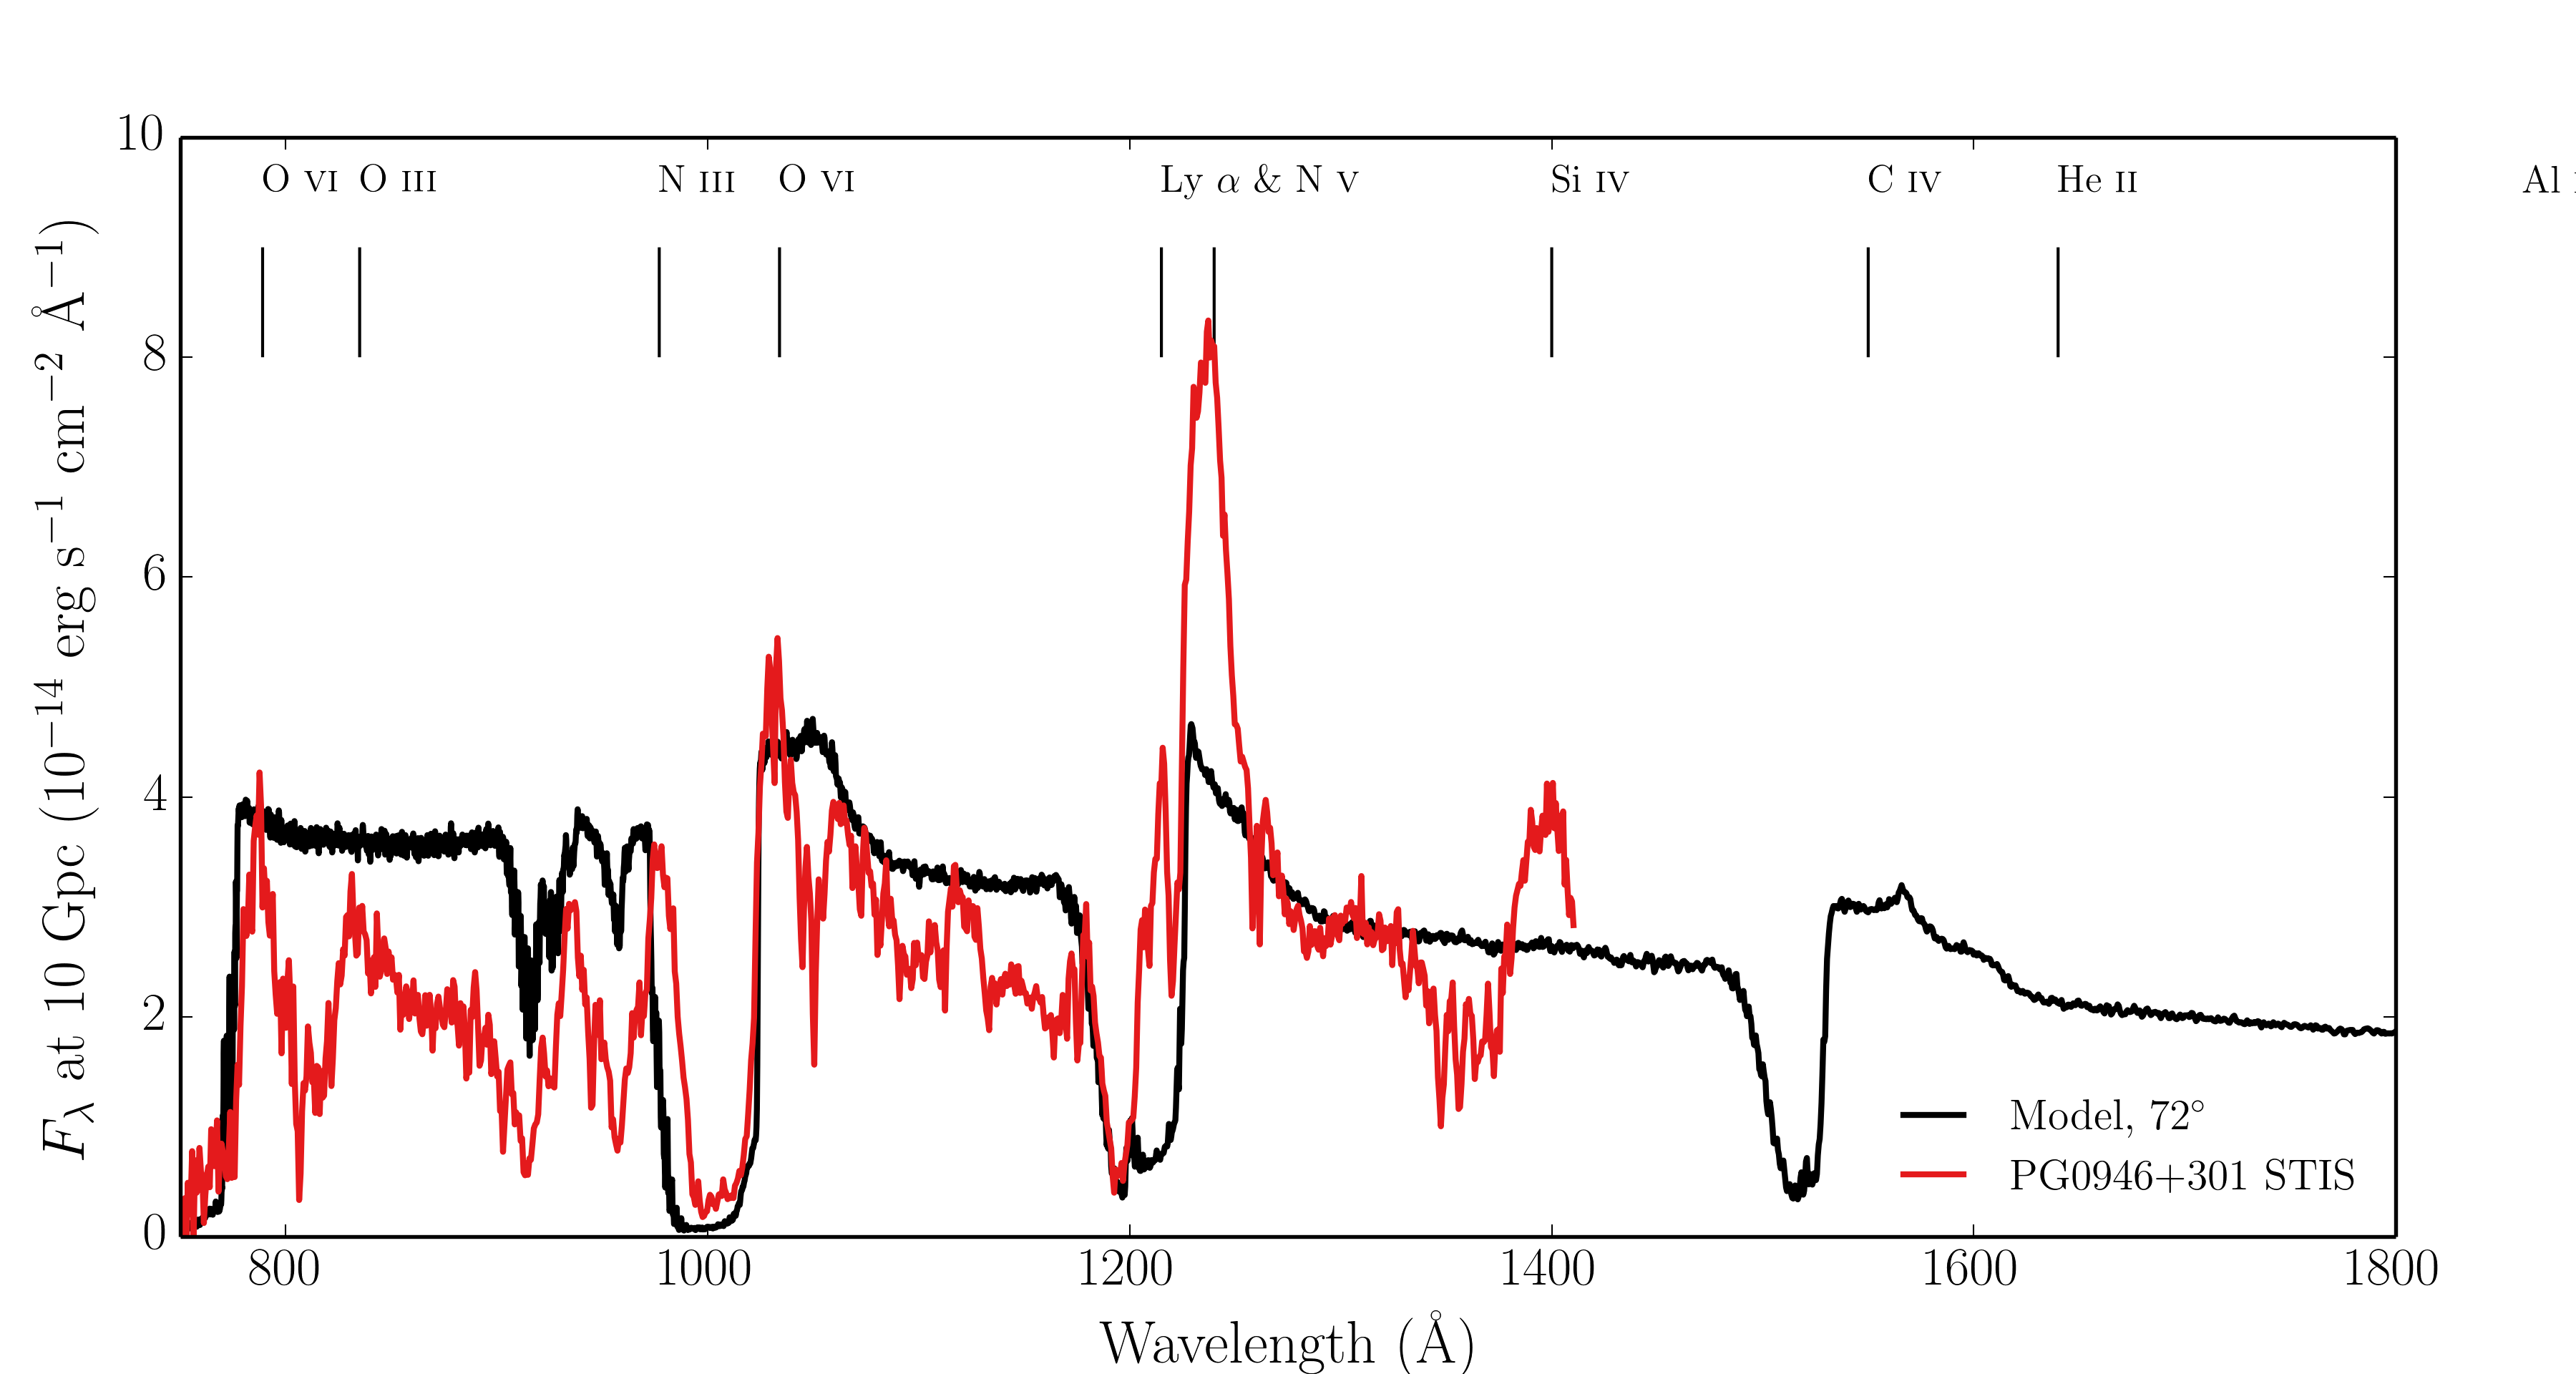
\includegraphics[width=1.0\textwidth]{figures/0946.png}
\caption
{
\DIFaddFL{Synthetic spectra at $72^\circ$ compared to an HST STIS spectrum
of PG0946+301 (Arav et al. 2000). The spectrum is scaled to the flux at 1300\AA}\
\DIFaddFL{for direct comparison. 
}}
\label{fig:stis}
\end{figure*} %DIF > fullpage
\DIFaddend 

Figure~\ref{fig:uvspec} shows the synthetic spectrum in the UV from our model. 
\DIFdelbegin \DIFdel{We also show a comparison to composite }\DIFdelend \DIFaddbegin \DIFadd{To assess the ability of the model to match real 
quasar spectra, we also show }{\sl \DIFadd{Sloan Digital Sky Survey}} \DIFadd{(SDSS) }\DIFaddend quasar and BALQSO 
\DIFdelbegin \DIFdel{spectra}\DIFdelend \DIFaddbegin \DIFadd{composites from \mbox{%DIFAUXCMD
\cite{reichard2003}
}%DIFAUXCMD
, normalised to the flux at 2000\AA}\ \DIFadd{in each panel}\DIFaddend . 
We show a cartoon illustrating how geometric effects determine
the output spectra in figure~\ref{fig:sightline}.  

\subsubsection{Broad absorption lines \DIFaddbegin \DIFadd{(`BALQSO-like' angles)}\DIFaddend }

The UV spectrum is characterised by strong BAL 
profiles at high inclinations ($> 70^\circ$). 
This highlights the first success of our model: 
clumping means the correct ionization state 
is maintained in the presence of strong X-rays, 
allowing large resonance line opacities. 
At the highest inclinations, the 
cooler, \DIFdelbegin \DIFdel{lower }\DIFdelend \DIFaddbegin \DIFadd{low }\DIFaddend ionization material at the base of the wind
starts to intersect the line of sight. This produces 
multiple absorption lines in \DIFdelbegin \DIFdel{lower ionization }\DIFdelend species such as \mg,
\al\ and Fe~\textsc{ii}. The potential links to LoBALQSOs and 
FeLoBALQSOs are discussed in section 2.4.
\DIFaddbegin \DIFadd{Clearly, the absorption lines in the 
synthetic spectra at BALQSO-like angles do not match the composites; this
is }{\em \DIFadd{not}} \DIFadd{due to a failure of our model, but rather because a geometric mean
BALQSO composite spectrum tends to wash out the broad absorption features due to the wide
range of absorption characteristics. To demonstrate this, we show a comparison 
to a }{\sl \DIFadd{Hubble Space Telescope}} \DIFadd{STIS spectrum of the high BALnicity BALQSO PG0946+301 
(Arav et al. 2000) in figure \ref{fig:stis}. 
}\DIFaddend 

The high ionization BAL profiles are often saturated, and the location in velocity space
of the strongest absorption in the profile varies with inclination.
At \DIFdelbegin \DIFdel{lower inclinations}\DIFdelend \DIFaddbegin \DIFadd{the lowest inclination BAL sightlines}\DIFaddend , the strongest absorption occurs at the red edge,
whereas at \DIFdelbegin \DIFdel{high }\DIFdelend \DIFaddbegin \DIFadd{higher }\DIFaddend inclinations (and for the strongest BALs)
the trough has a sharp edge at the terminal velocity.
This offers one potential explanation for the wide range of BALQSO absorption
line shapes (see e.g. Trump et al. 2006; Knigge et al 2008\DIFaddbegin \DIFadd{, Filiz Ak et al. 2014}\DIFaddend ).
In addition, the line profile shape is strongly dependent 
on the density, ionization and velocity 
profiles intersected by the line of sight. Thus, small tweaks of the velocity
law and angular distributions of streamlines can dramatically alter
the shape of the line.

Nonblack saturation is observed in the absorption troughs of BALQSOs \citep{arav1999a,arav1999b}.
This can be caused either by partial covering of the continuum
source or by scattered contributions to the BAL troughs, necessarily
from an opacity source not cospatial with the BAL forming region.
The scattered light explanation is supported by spectropolarimetry results
\citep{lamy2000}. Our spectra do not show nonblack saturation.
Instead, we find black, saturated troughs at angles $i > 73^\circ$, and the BALs
are non-saturated at lower inclinations. The reasons for this are readily apparent. 
First, the microclumping assumption does not allow for 
porosity in the wind, meaning that it does not naturally produce
a partial covering absorber. To do this, an alternative approach
such as {\em macroclumping} would be required \citep[e.g.][]{surlan2012,hamann2008}.
Second, our wind does not have a significant scattering 
contribution along sightlines which do not pass through the BAL region,
meaning that any scattered \DIFdelbegin \DIFdel{contribution is obscured by the saturated troughs }\DIFdelend \DIFaddbegin \DIFadd{component to the BAL troughs is absorbed by line opacity}\DIFaddend .
This suggests that either the scattering cross-section of the wind must
be increased (with higher mass loss rates or covering factors), or 
that an additional source of electron opacity is required, potentially
in a polar direction above the disc.


\subsubsection{Broad emission lines \DIFaddbegin \DIFadd{(`quasar-like' angles)}\DIFaddend }

\DIFdelbegin \DIFdel{We find that the model can produce significant line emission
}\DIFdelend \DIFaddbegin \begin{figure*} %DIF > fullpage
\centering
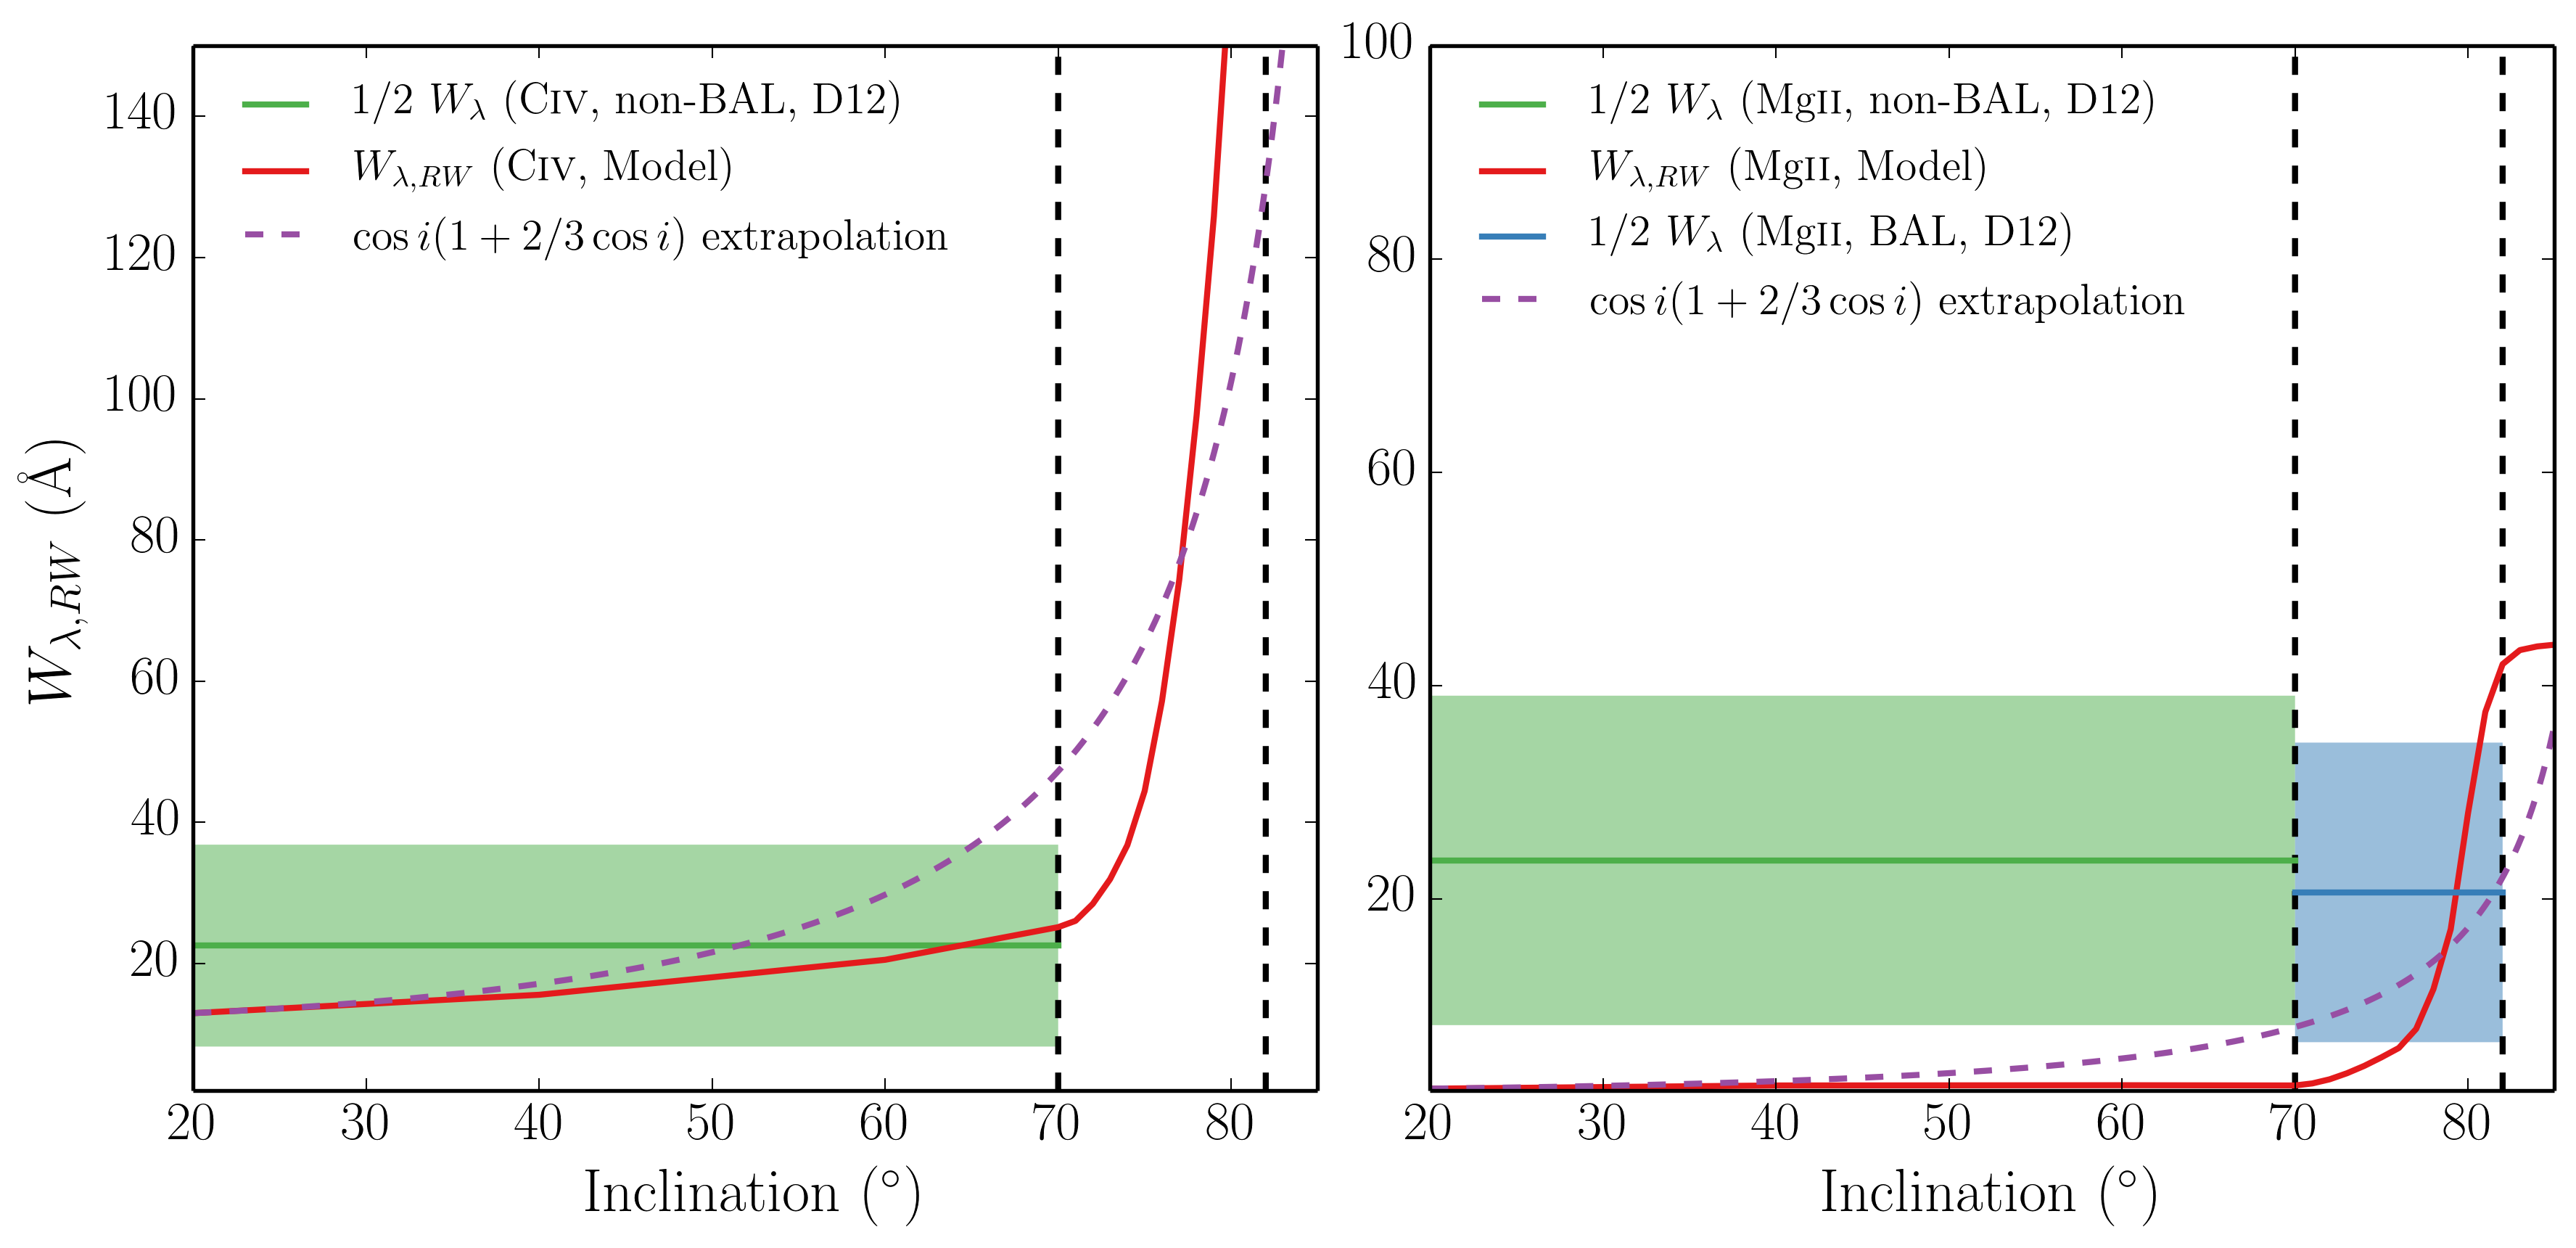
\includegraphics[width=1.0\textwidth]{figures/ew.png}
\caption
{
\DIFaddFL{Physical properties of the outflow, shown by the coloured contours.
The solid black line marks a sphere at $1000~r_G$.
The dotted lines show the $72^\circ$ and $78^\circ$ sightlines 
to the centre of the system, and illustrate that different sightlines
intersect material of different ionization states.
}}
\label{fig:ew}
\end{figure*} %DIF > fullpage

\DIFadd{We find significant collisionally excited line emission emerges
}\DIFaddend at low inclinations \DIFaddbegin \DIFadd{in the synthetic spectra}\DIFaddend , particular in \DIFaddbegin \DIFadd{the }\DIFaddend \civ\DIFdelbegin \DIFdel{, 
and the }\DIFdelend \DIFaddbegin \ \DIFadd{line.
The }\DIFaddend improved treatment of recombination \DIFaddbegin \DIFadd{also }\DIFaddend results in a strong \la\ line. 
In the context of unification, this is a promising result, 
and shows that a biconical wind can produce significant 
emission at `quasar-like' angles. 
\DIFdelbegin \DIFdel{To assess the ability of the model to match real 
quasar spectra , we also show }%DIFDELCMD < {\sl %%%
\DIFdel{Sloan Digital Sky Survey}%DIFDELCMD < } %%%
\DIFdel{(SDSS) quasar composites from
\mbox{%DIFAUXCMD
\cite{reichard2003}
}%DIFAUXCMD
, normalised to the flux at 2000\AA}%DIFDELCMD < \ %%%
\DIFdel{in each panel.
We do not produce the semi-forbidden 
intercombination lines seen in quasar spectra because we
currently do not have a treatment for semi-forbidden lines.
This is especially noticable with the }\DIFdelend \DIFaddbegin \DIFadd{The spectra do not contain the }\DIFaddend strong C~\textsc{iii}]~1909\AA\, 
line \DIFaddbegin \DIFadd{seen }\DIFaddend in the quasar composite spectra. 
\DIFaddbegin \DIFadd{This is because we do not yet treat C as a full macro-atom with a 
full collisional rates between forbidden
or semi-forbidden transitions, as would be required.
}\DIFaddend The critical density of the C~\textsc{iii}]~1909\AA\, line 
is $n_e\sim10^{9.5}~\rm{cm^{-3}}$ \DIFaddbegin \DIFadd{\mbox{%DIFAUXCMD
\citep{wei1988}
}%DIFAUXCMD
}\DIFaddend , which is higher than much of the 
outer portion of our wind. 
We therefore expect \DIFdelbegin \DIFdel{intercombination lines
to become important coolants in the outer portion of the wind}\DIFdelend \DIFaddbegin \DIFadd{a model with these 
parameters to produce a C~}\textsc{\DIFadd{iii}}]\DIFadd{~1909\AA}\ \DIFadd{line
with a proper treament}\DIFaddend . 

The model produces strong emission lines in \civ, \nv\ and \la,
as well as a weak \mg\ line. The shapes and widths of these lines
match the composites fairly well. However, the line-to-continuum ratios 
at low inclinations in our model are significantly weaker than the quasar 
composites. Increasing the density of the outflow, by altering the mass 
loss rate  or velocity law, can produce more line emission.
However, the red wing of the BAL profiles is generally stronger than 
seen in BALQSO spectra and composites. This illustrates a fundamental 
problem with a geometric unification model such as this:
that the line-to-continuum ratios at \DIFdelbegin \DIFdel{low }\DIFdelend \DIFaddbegin \DIFadd{hight }\DIFaddend inclinations are
significantly affected by disc foreshortening and limb darkening.
The angular distribution of the disc radiation is clearly
crucially important in determining the emergent line ratios.

\subsubsection{The \DIFdelbegin \DIFdel{Disc SED}\DIFdelend \DIFaddbegin \DIFadd{Angular Distribution of Line And Continuum Emission}\DIFaddend }
\DIFdelbegin %DIFDELCMD < \label{discsed}
%DIFDELCMD < %%%
\DIFdelend \DIFaddbegin \label{angular}
\DIFaddend 

\DIFdelbegin %DIFDELCMD < \begin{figure}
%DIFDELCMD < \centering
%DIFDELCMD < 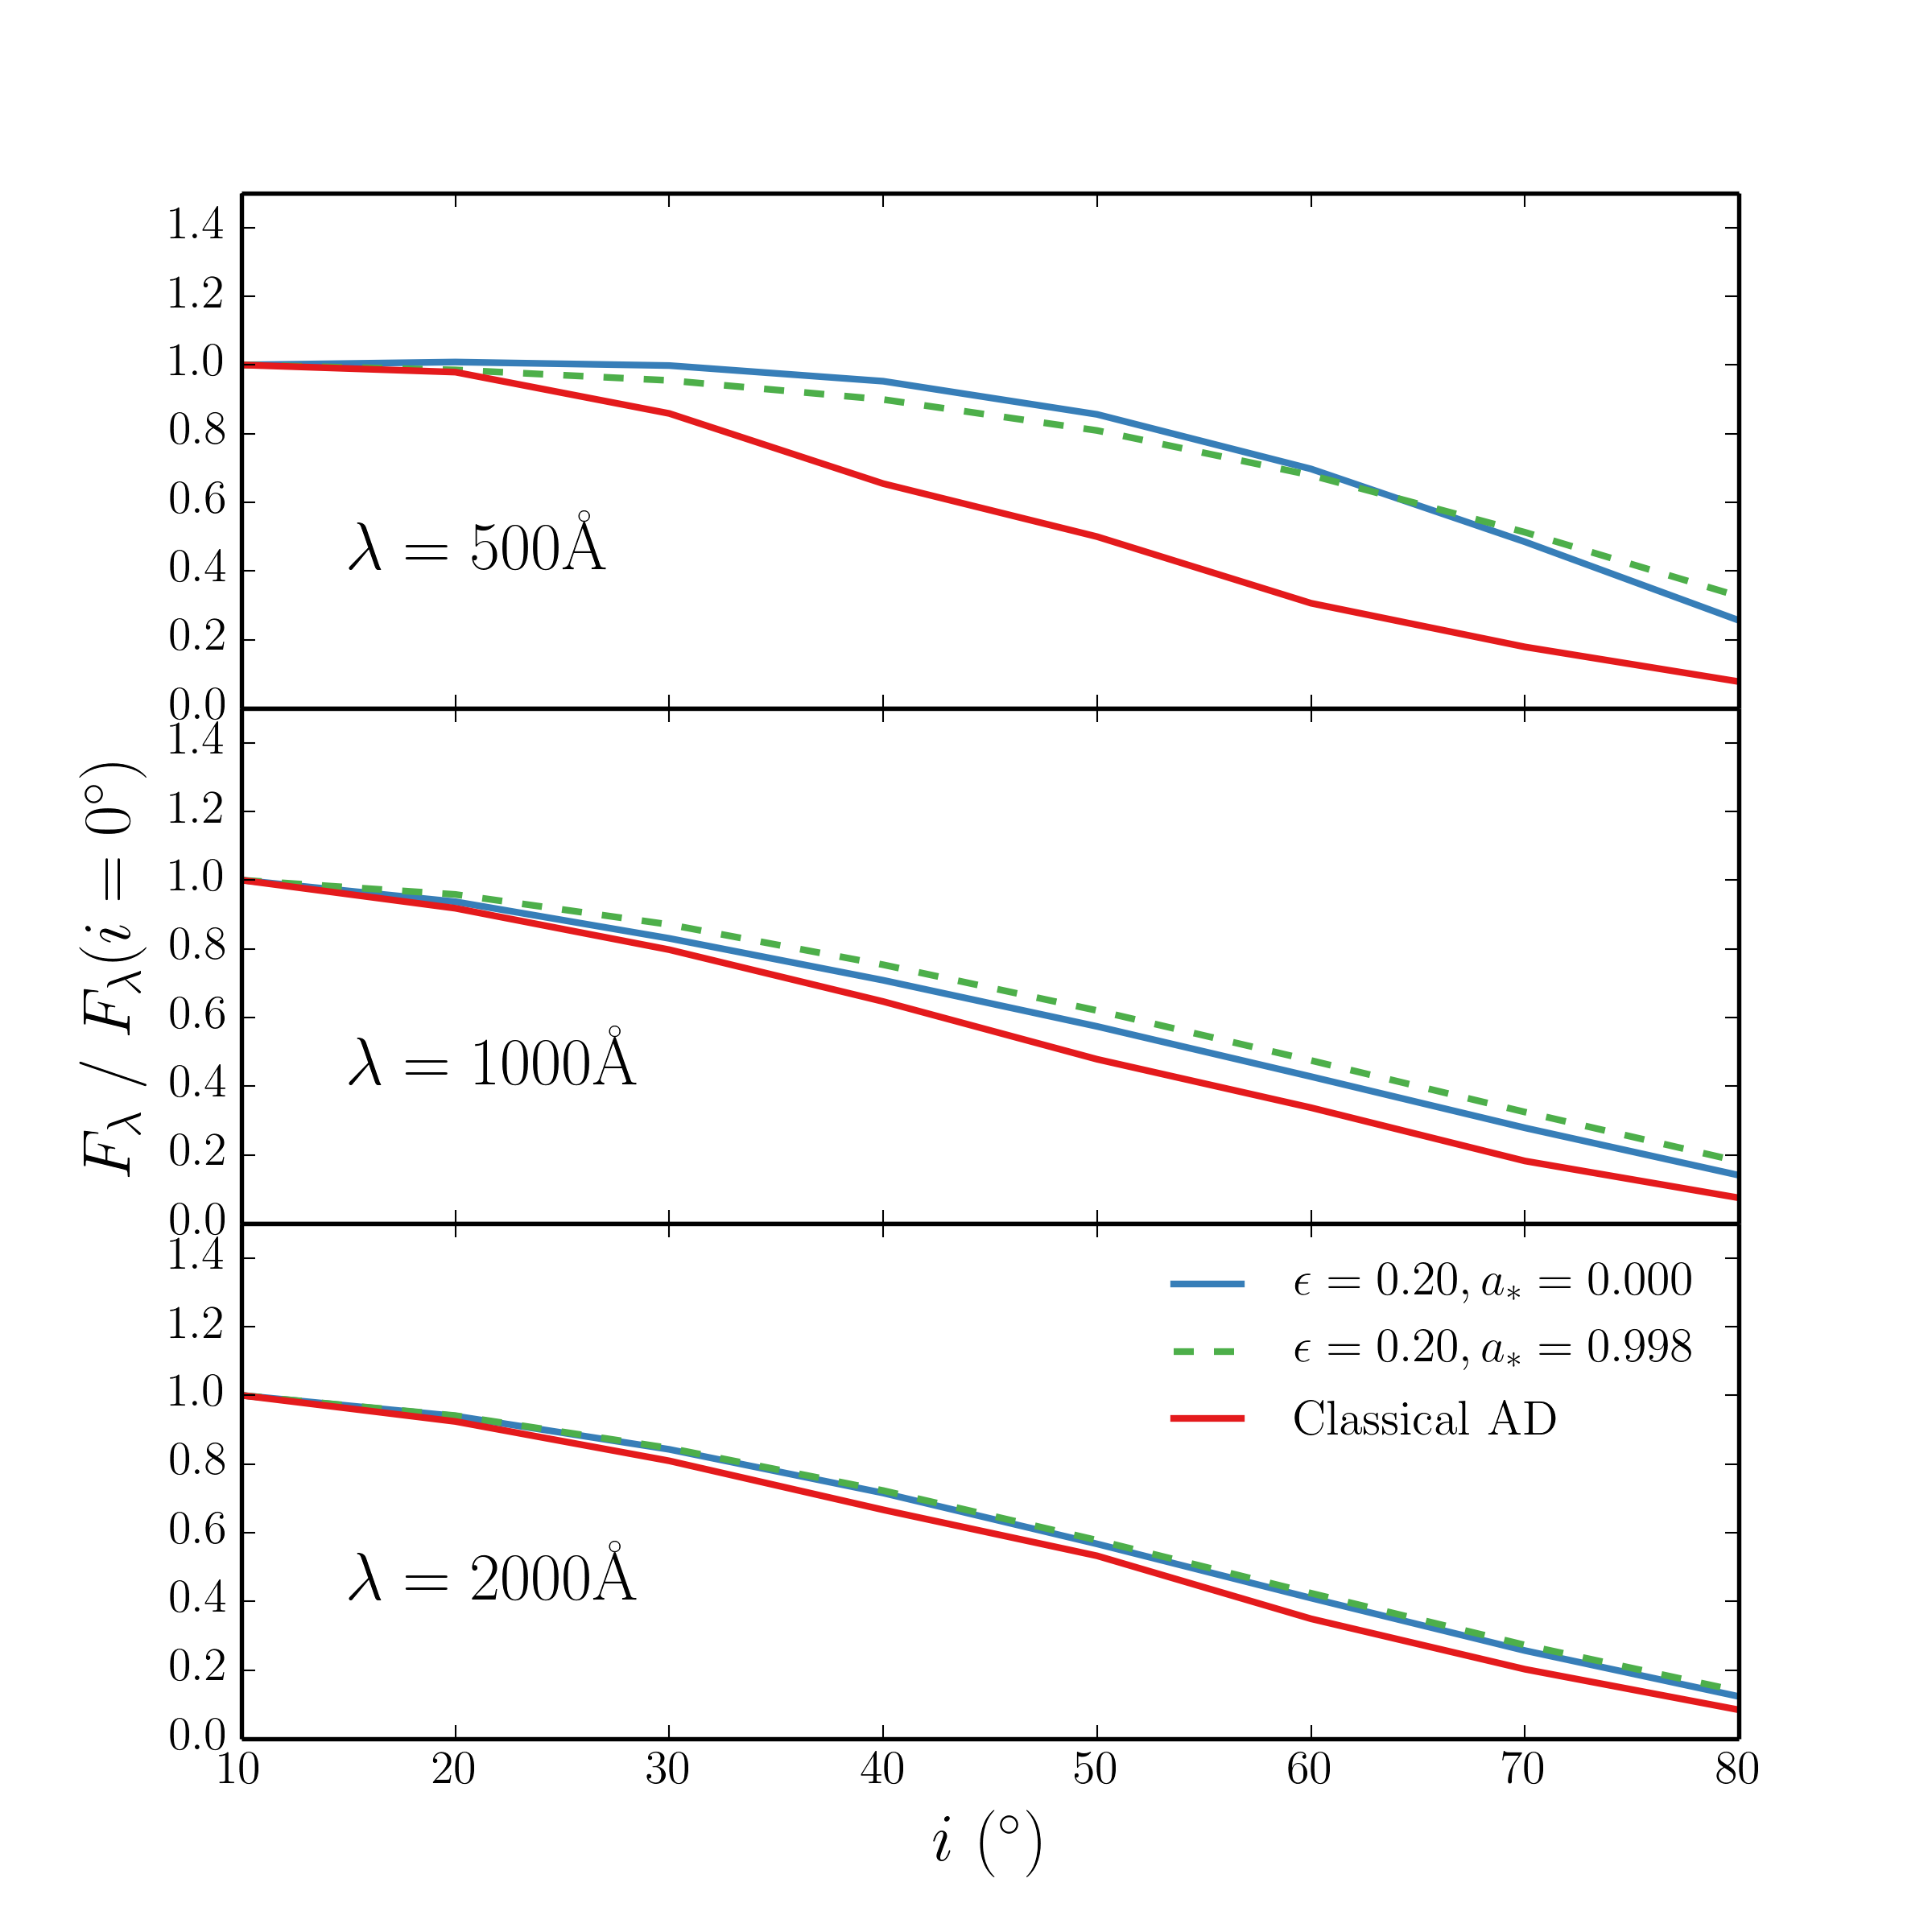
\includegraphics[width=0.5\textwidth]{figures/agnspec.png}
%DIFDELCMD < \caption
%DIFDELCMD < {
%DIFDELCMD < %%%
\DIFdel{$F_\lambda$ for three different wavelengths
as a function of inclination from }%DIFDELCMD < \agn%%%
\DIFdelend \DIFaddbegin \DIFadd{In order to quantitatively assess how emission lines change with 
inclination when blue-shifted absorption 
may affect the line profile, we define the `red wing equivalent width' ($W_{\lambda,RW}$) as
}\begin{equation}\DIFadd{
W_{\lambda,RW} = \int_{\lambda_0}^{\lambda^\prime} \left( 1 - \frac{F_\lambda}{F_0} \right) d\lambda
\label{rwew}
}\end{equation}
\DIFadd{where $F_0$ is the continuum flux and the integral is calculated from $\lambda_0$, line centre,
to a wavelength $\lambda^\prime$ where the flux has returned to the continuum level.
This quantity is shown as a function of inclination in figure 5 for the }\civ\ \DIFadd{and }\mg\DIFaddend \ \DIFdelbegin \DIFdel{models, compared to a classical AD.
The }%DIFDELCMD < \agn\ %%%
\DIFdel{models are computed 
for Kerr and Scharzschild BHs with the same $M_{BH}$ and $\dot{m}$ as our model. 
}%DIFDELCMD < }
%DIFDELCMD < \label{fig:f2000}
%DIFDELCMD < \end{figure}
%DIFDELCMD < %%%
\DIFdelend \DIFaddbegin \DIFadd{UV lines.
We also plot show the $W_{\lambda,RW}$ expected from isotropic line emission and a foreshortened 
and limb darkened disc  as well as $1/2$ equivalent widths from \mbox{%DIFAUXCMD
\cite{dipompeo2012b}
}%DIFAUXCMD
. 
}\DIFaddend 

\DIFdelbegin \DIFdel{When comparing BALQSO and quasar composites, it is apparent
that they possess remarkably similar line strengths and widths 
\mbox{%DIFAUXCMD
\citep[e.g.][]{weymann1991,reichard2003}
}%DIFAUXCMD
. 
}\DIFdelend \DIFaddbegin \DIFadd{BALQSOs and quasars generally possess very similar emission line properties 
\mbox{%DIFAUXCMD
\citep[e.g.][]{weymann1991,reichard2003}
}%DIFAUXCMD
. 
Clearly, the variation with inclination in our models is far greater than 
than the variation between, and standard deviation within, quasar and BALQSO samples.  
}\DIFaddend This presents a challenge to our model, as well as the geometric unification picture in general.
\DIFdelbegin \DIFdel{Limb darkening and foreshortening causes the disc continuum emission to be 
strongly anisotropic, yet the line emission in our models is much more isotropic . 
This has the effect of enhancing the line-to-continuum ratios at high inclinations. 
To construct a scenario where emission 
line equivalent widths are comparable at all inclinations requires 
significant fine-tuning when considering a }\DIFdelend \DIFaddbegin \DIFadd{One obvious potential solution is to hypothesize a more isotropic distribution 
for the emergent condition than predicted by a }\DIFaddend classical thin disc. 
\DIFdelbegin \DIFdel{An alternative, simpler solution is that the emergent continuum is roughly isotropic.
}%DIFDELCMD < 

%DIFDELCMD < %%%
\DIFdelend General relativistic effects -- specifically, light bending
and relativistic beaming -- can cause 
the accretion disc SED to become more isotropic \citep[e.g.][]{zhang1997,munozdarias2013}. 
\DIFdelbegin \DIFdel{To generate GR disc spectra, we use the code }%DIFDELCMD < \agn\ %%%
\DIFdel{\mbox{%DIFAUXCMD
\citep{hubeny2000,davishubeny2006,davis2007}
}%DIFAUXCMD
. 
The output flux at three different wavelengths
as a function of inclination for an }%DIFDELCMD < \agn\ %%%
\DIFdel{model with the same disc and BH parameters
as our clumpy wind model is shown in figure~\ref{fig:f2000}.
The effects of GR on an AGN disc are much less extreme 
in the UV portion of the spectrum than the calculations
by \mbox{%DIFAUXCMD
\cite{zhang1997}
}%DIFAUXCMD
for the X-rays in X-ray binaries.
As a result, 
}\DIFdelend \DIFaddbegin \DIFadd{However, we have verified using AGNSPEC \mbox{%DIFAUXCMD
\citep{hubeny2000,hubeny2001,hubenyhubeny1997}
}%DIFAUXCMD
that this effect is small in }\DIFaddend the \DIFdelbegin \DIFdel{disc emission is still strongly anisotropic.
GR alone therefore cannot explain the line ratio trends in quasars by making the disc
emit more isotropically.
This supports the findings of \mbox{%DIFAUXCMD
\cite{risaliti2011}
}%DIFAUXCMD
, who }\DIFdelend \DIFaddbegin \DIFadd{UV and optical wavelength regimes, 
and the disc is still anisotropic.
}

\DIFadd{Reprocessing by an extended outflow may also cause a more isotropic
continuum to emerge. Hints that light scattered off a spatially extended 
wind may contribute signiciantly to the emergent continuum come from radiative transfer s
simulations \mbox{%DIFAUXCMD
\citep{simproga2012}
}%DIFAUXCMD
and microlensing observations \mbox{%DIFAUXCMD
\citep{sluse2015}
}%DIFAUXCMD
.
However, neither of these examples have sufficient reprocessing efficiencies to 
compensate for the disc anisotropy in this case.
An alternative explanation is that the BLR has the same angular distribution 
of emission as the accretion disc.
Indeed, \mbox{%DIFAUXCMD
\cite{risaliti2011}
}%DIFAUXCMD
}\DIFaddend find that EW distributions in quasars are consistent with anisotropic emission 
from optically thick, disc-like structures for {\em both} the continuum source and BLR. 
If this is the case, it has a dramatic affect on the intrinsic
BAL fraction inferred from flux-limited samples \citep{goodrich1997,krolikvoit1998}. 
\DIFdelbegin \DIFdel{We will explore these ideas further in a future study}\DIFdelend \DIFaddbegin 

\DIFadd{It is also possible that the equatorial paradigm invoked from early polarisation
studies \mbox{%DIFAUXCMD
\citep{goodrich1995, cohen1995,brotherton2006}
}%DIFAUXCMD
is an over-simplification, or is merely incorrect. 
High brightness temperatures in some RL BALQSOs imply polar outflows \mbox{%DIFAUXCMD
\citep{zhou2006}
}%DIFAUXCMD
and \mbox{%DIFAUXCMD
\cite{bruni2012}
}%DIFAUXCMD
find that
RL BALQSOs possess similar radio spectral indices to normal RL quasars, 
suggestive of comparable inclinations. 
In addition, \mbox{%DIFAUXCMD
\cite{marin2013}
}%DIFAUXCMD
find a bending angle of $\sim45^\circ$ is required to 
explain the polarisation dichotomy of type 1 and 2 AGN using an Elvis-type wind 
model (Elvis 2000). It is therefore possible 
that type 1 quasars and BALQSOs are generally viewed from a fairly narrow range of angles 
($\sim0$-$45^\circ$), or that }{\em \DIFadd{both}} \DIFadd{evolutionary and geometric explanations are required.
We suggest that future modelling should include predictions of polarisation signatures
from a detailed radiative transfer simulation, allowing direct comparison with spectropolarimetry
of BALQSOs}\DIFaddend . 


%DIF >  The final possibility is that BALQSOs are not viewed equatorially. 
%DIF >  This possibility is supported by measurements of the radio spectral indices
%DIF >  of radio-loud BALQSOs (REF) and attempts to explain the polarisation dichotomy 
%DIF >  of type 1 and 2 AGN (REF). This would imply that type 1 quasars and BALQSOs are generally 
%DIF >  viewed from a fairly narrow range of angles ($\sim0$-$50^\circ$), and could also mean 
%DIF >  the BALQSO fraction requires {\em both} evolutionary and geometric explanations. 
%DIF >  There is also clear conflict between this explanation and some
%DIF >  polarisation results \citep{goodrich1995, cohen1995}(BROTHERTON).
%DIF >  We suggest that future modelling should include predictions of polarisation signatures
%DIF >  from a detailed radiative transfer simulation, allowing 
\DIFaddbegin 



%DIF >  When comparing BALQSO and quasar composites, it is apparent
%DIF >  that they possess remarkably similar line strengths and widths 
%DIF >  \citep[e.g.][]{weymann1991,reichard2003}.  
%DIF >  {\bf I think we mean EW here; otherwise I don't understand what we are talking about.  We could say ``line shapes and equivalent widths''.  I also think this requries more than one sentence of introduction.} This presents a challenge to our model, as well as the geometric 
%DIF >  unification picture in general, because these quantities should vary with inclination angle.
%DIF >  Limb darkening and foreshortening causes the disc continuum emission to be 
%DIF >  strongly anisotropic, yet the line emission in our models is much more isotropic. 
%DIF >  This has the effect of enhancing the line-to-continuum ratios at high inclinations. 
%DIF >  To construct a scenario where emission 
%DIF >  line equivalent widths are comparable at all inclinations requires 
%DIF >  significant fine-tuning when considering a classical thin disc. {\bf Is the previous sentence a throwaway line, or has some person done this.  If so, please reference; if not please delete.}
%DIF > An alternative, simpler solution is that the emergent continuum is roughly isotropic.

%DIF >  Obviously,  one possible solution to this problem is hypothesize a more isotropic distribution for the emergent condition than predicted by a ``classical'' disc. 
%DIF >  General relativistic effects -- specifically, light bending
%DIF >  and relativistic beaming -- can cause 
%DIF >  the accretion disc SED to become more isotropic \citep[e.g.][]{zhang1997,munozdarias2013}.  Incorporating these effects into {\sc PYTHON} would be a very difficult and time-consuming challenge. Therefore, for the purposes of this discussion we have chosen to investigate whether GR effects could produce enough isotropy to address the EW problem, we have generated 
%DIF >  \ GR disc spectra, we use the code \agn\ \citep{hubeny2000,davishubeny2006,davis2007}. 
%DIF >  The output flux at three different wavelengths
%DIF >  as a function of inclination for an \agn\ model with the same disc and BH parameters
%DIF >  as our clumpy wind model is shown in figure~\ref{fig:f2000}.  The results indicate that 
%DIF >  the effects of GR on an AGN disc are much less extreme 
%DIF >  in the UV portion of the spectrum than the calculations
%DIF >  by \cite{zhang1997} for the X-rays in X-ray binaries.
%DIF >  The emission for the disks of AGN is still strongly anisotropic.
%DIF >  GR alone therefore cannot explain the line ratio trends in quasars by making the disc
%DIF >  emit more isotropically. This supports the findings of \cite{risaliti2011}, 
%DIF >  who find that EW distributions in quasars are consistent with anisotropic emission 
%DIF >  from optically thick, 
%DIF >  disc-like structures for {\em both} the continuum source and BLR. 
%DIF >  If this is the case, it has a dramatic affect on the intrinsic
%DIF >  BAL fraction inferred from flux-limited samples \citep{goodrich1997,krolikvoit1998}.
%DIF >  We will explore these ideas further in a future study.  
%DIF >  {\bf Wait!  All this says is that there has to be an alternative explanation.
%DIF >  It is not support for any specific explanation!. This last few sentences should
%DIF >  be a separate paragraph.  They should start out: An alernative explanation proposed 
%DIF >  by risalite is that...}

\DIFaddend % Figure 5 also shows the spectrum into the optical,
% showing that the outflow produces signiciant optical emission lines
% as well as having a noticeable effect on the continuum shape. This
% is particularly true around the Balmer jump at $3646\AA$ and is due to
% a prominent wind-formed recombination continuum.


\subsection{X-ray Properties and Broadband SEDs}
\DIFaddbegin \label{sec:xray}
\DIFaddend 


\begin{figure*} %fullpage
\centering
\DIFdelbeginFL %DIFDELCMD < 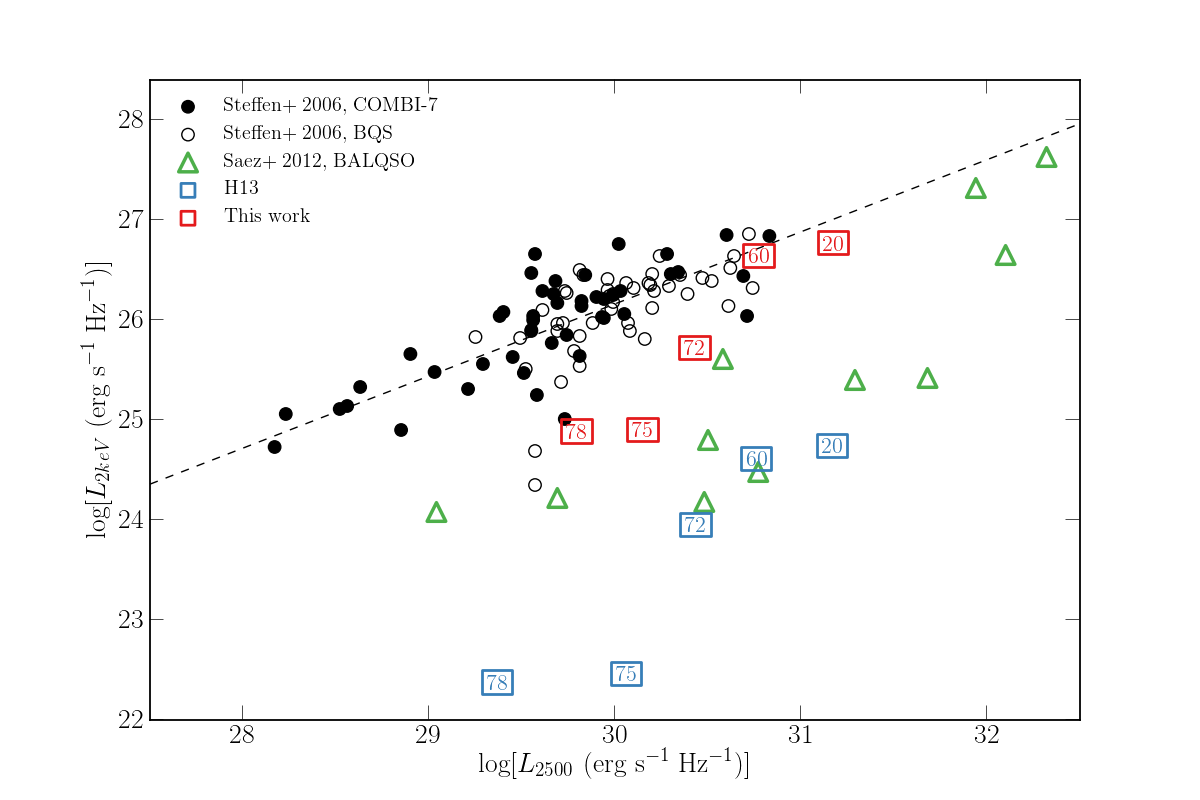
\includegraphics[width=1.0\textwidth]{figures/lx.png}
%DIFDELCMD < %%%
\DIFdelendFL \DIFaddbeginFL 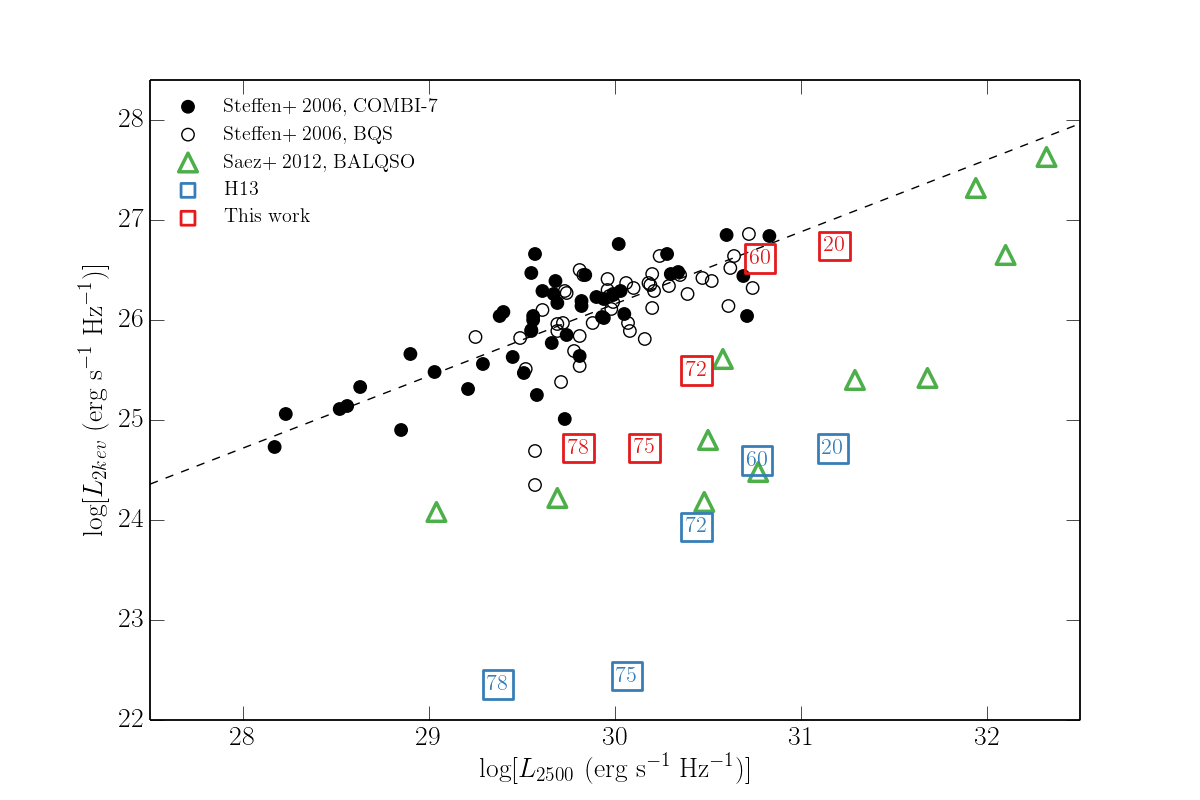
\includegraphics[width=1.0\textwidth]{figures/lx_a05_pre.png}
\DIFaddendFL \caption
{
X-ray ($2$~keV) luminosity of the our clumped model (red squares) 
and the H13 model (purple squares), plotted against monochromatic luminosity 
at 2500\AA. The points are labeled according to inclination; angles
$>70^\circ$ correspond to BALs in our scheme (see figure 4).
Also plotted are the samples considered by Saez et al. 2012 on a similar plot; 
The COMBI-7 AGN and the BQS samples Steffen et al. (2006) and the Saez et al. (2012) 
sample of BALQSOs. The dotted line shows the best fit relation for non-BALQSOs 
from Steffen et al. (2006).
}
\label{fig:xray}
\end{figure*} %fullpage

% \begin{figure} %fullpage
% \centering
% 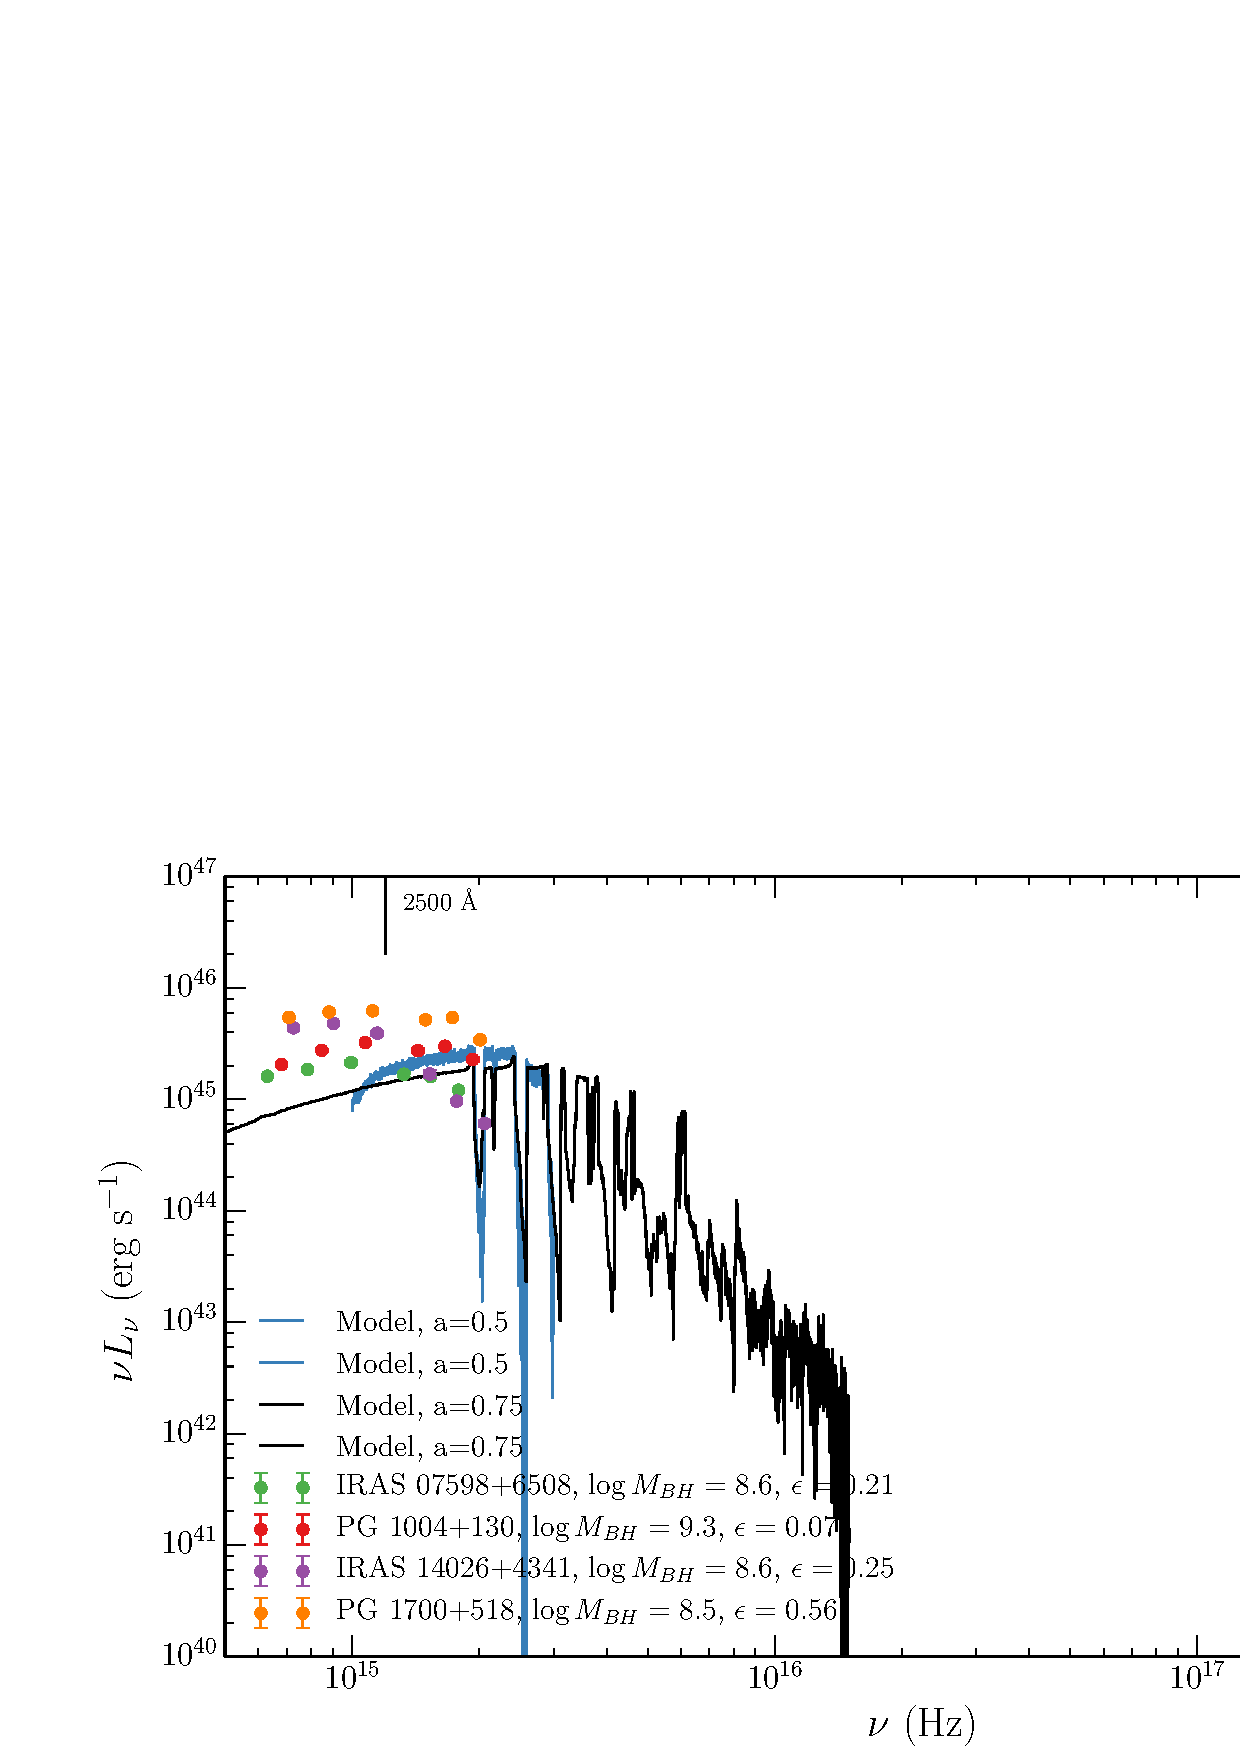
\includegraphics[width=1.0\textwidth]{figures/sed_all_balqsos.png}
% \caption
% {
% Broadband SEDs compared to IR and X-ray SEDs for selected BALQSOs 
% from Grupe \& Nousek (2015).
% }
% \label{fig:xray}
% \end{figure} %fullpage

%DIF > {\bf:  Again this section needs an introduction.  Why is this important?}
\DIFaddbegin 

\DIFadd{One of the main motivations for including a treatment of clumping was
to avoid over-ionization of the wind in the presence of strong X-rays. 
Having verified that strong BALs appear in the synthetic spectra,
it is also important to assess whether the X-ray properties of this
next-generation model agree well with quasar and BALQSO samples for the relevant
inclinations.
}

\DIFaddend Figure~\ref{fig:xray} shows the emergent
monochromatic luminosity ($L_\nu$) at 2~keV and 
%$\alpha_{OX}$ 
plotted against $L_\nu$ at $2500$\AA\ for a number of different viewing angles in our model.
% $\alpha_{OX}$ is a spectral index from near UV to X-rays defined by
% \begin{equation}
% \alpha_{OX}=0.3838\log\left(\frac{L_{\nu}(2~keV)}{L_{\nu}(2500~\mbox{\scriptsize{\AA}})}\right),
% \end{equation}
% which effectively represents a near-UV to X-ray flux ratio and a measure of X-ray 
% weakness. 
The monochromatic luminosities are calculated from the synthetic spectra and thus include
the effects of wind reprocessing and attenuation. In addition to model outputs,
we also show the BALQSO sample of Saez et al. (2012) and luminous AGN and quasar
samples from Steffen et al. (2006). The best fit relation from Steffen et al. (2006) 
is also shown. For low inclination, `quasar-like' viewing angles,
we now \DIFdelbegin \DIFdel{show }\DIFdelend \DIFaddbegin \DIFadd{find }\DIFaddend excellent agreement with AGN samples. The gradient from $20^\circ$ to
$60^\circ$ in our models is caused by a combination of disc foreshortening/limb-darkening 
(resulting in a lower $L_{2500}$ for higher inclinations) and the fact that the disk 
is opaque, and thus the X-ray source subtends a smaller solid angle at high inclinations
(resulting in a lower $L_{2keV}$ for higher inclinations). 



The low inclination, `BALQSO-like' viewing angles show moderate agreement with the data,
and are X-ray weak due to bound-free and electron scattering opacities in the wind.
Typically, BALQSOs show strong X-ray absorption with columns 
of $N_H\sim10^{23}~\rm{cm^{-2}}$ 
\citep{green1996,mathur2000,green2001,grupemathur2003}.
This is often cited as evidence that the BAL outflow is shielded from
the X-ray source, especially as sources with strong X-ray absorption tend
to exhibit deep BAL troughs and high outflow velocities 
\citep{brandt2000,laorbrandt2002,gallagher2006}.
Our results imply that the clumpy BAL outflow
itself can be responsible for the strong X-ray absorption, 
and supports Hamann et al.'s (2013) suggestion that 
this explains the weaker X-ray absorption in mini-BALs 
compared to BALQSOs.

Our models slightly over-predict the emergent X-ray luminosity at BAL angles, 
although we are limited by poor sample sizes. 
% It is possible that this is due to our wind being overly optically thick to 
% electron scattering at angles which look through the wind. 
If BALQSOs were {\em intrinsically} 
X-ray weak \citep[as suggested by, e.g.][]{morabito2013},
our isotropic assumption \DIFdelbegin \DIFdel{foe }\DIFdelend \DIFaddbegin \DIFadd{for }\DIFaddend the X-ray source would be incorrect. 
A polar-biased X-ray source would result in a lower clumping factor being
required in our model. Our specific wind
prescription will also affect the opacities, densities and resultant
ionization structure, which can change the absorption characteristics and resultant
luminosities.
Nevertheless, our input X-ray spectrum
now reproduces the X-ray properties of a luminous quasar as an output,
and at least some BAL angles match the observations.
This satisifies the first-order requirement for the X-ray properties of 
a unified quasar model.

% We can also examine the emergent X-ray spectra from our model. 
% Our code is not yet optimized for producing X-ray spectra, as we do not yet 
% include all lines and levels of e.g. Fe or macro-atom treatments of 
% higher order ions (cf. Sim et al. 2008, 2010). 
% However, the bound-free opacity sources are complete, and comparisons of the shape
% of the heavily absorbed spectra can be useful.
% Figure 6 shows the broadband SED from the model, compared to a number of BALQSO spectra
% from \cite{grupenousek2015} - note that lower mass and super-Eddington sources
% are excluded. 

% discuss the figure showing X-ray properties briefly. 
% Present an X-ray spectrum? compare to observations e.g. Giustini?

% {\bf Figures 5 and 6: $L_{2kev}$ v $L_{2500}$ plot and X-ray spectrum compared to Grupe and Nousek (broadband SED?)} 

\subsection{LoBALs and ionization stratification}

\begin{figure*} %fullpage
\centering
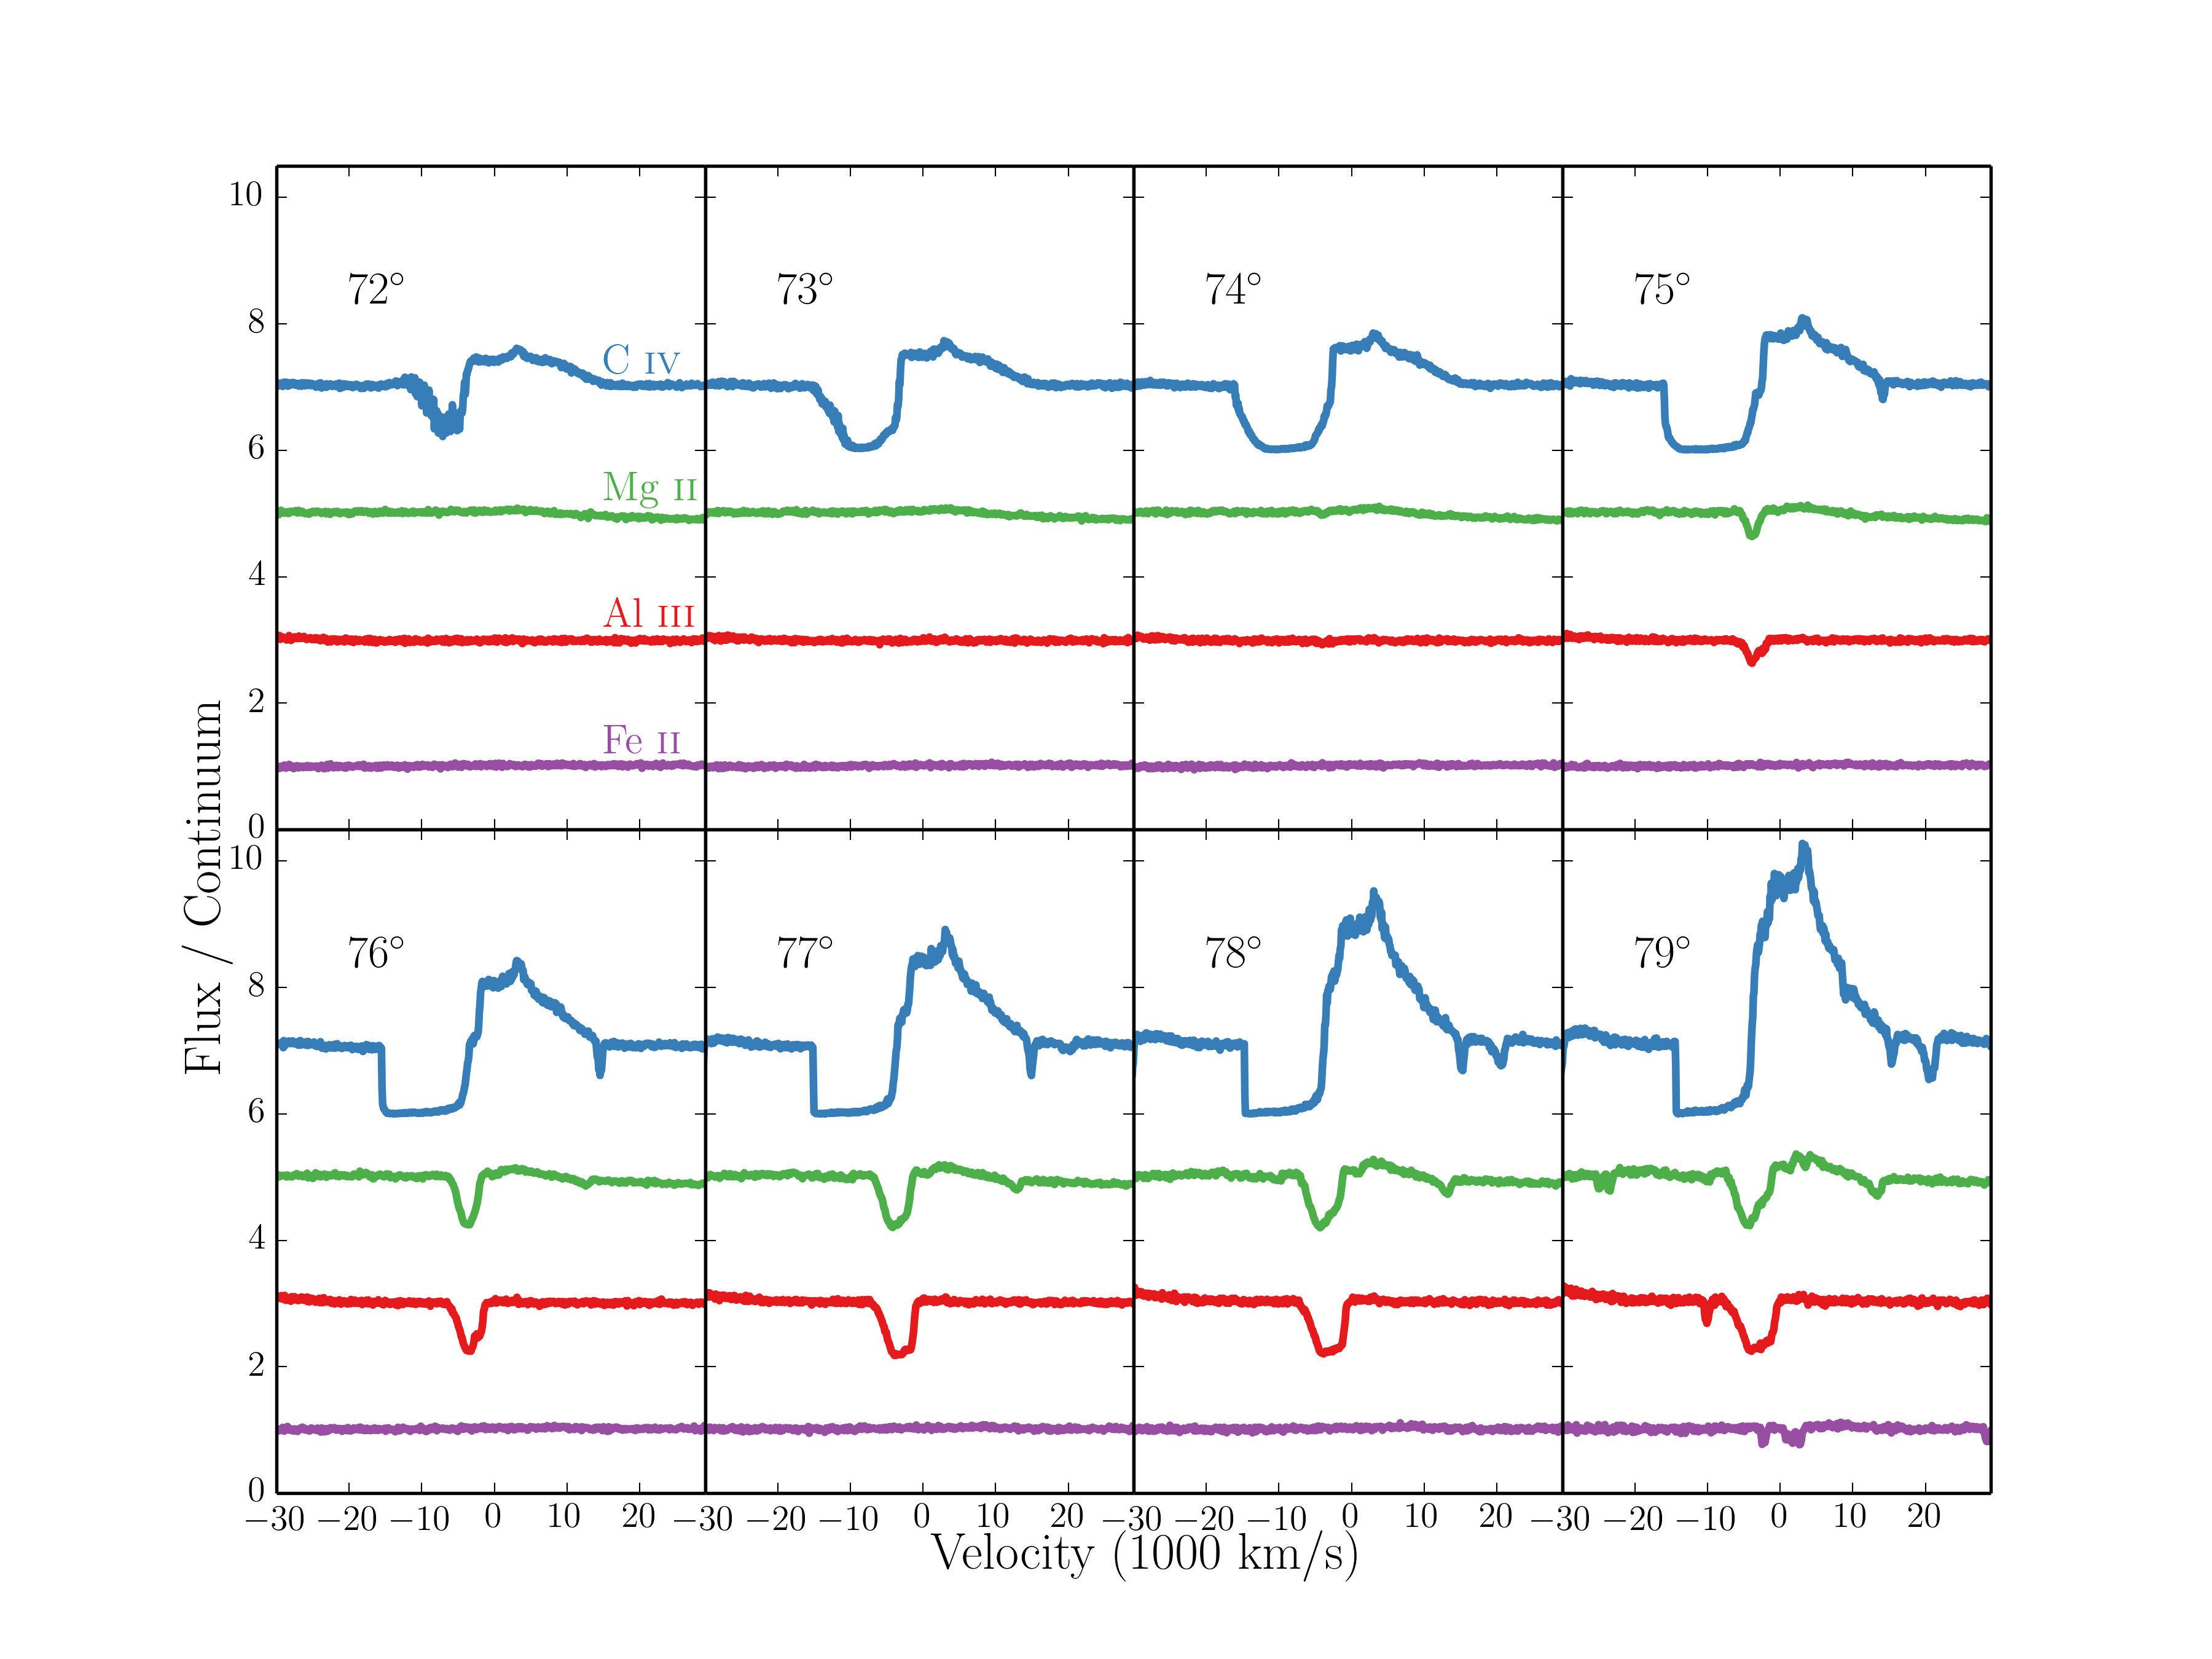
\includegraphics[width=1.0\textwidth]{figures/c4_angles.png}
\caption
{
\civ , \mg , \al\ and Fe~\textsc{ii} line profiles for \DIFdelbeginFL \DIFdelFL{wind }\DIFdelendFL \DIFaddbeginFL \DIFaddFL{viewing }\DIFaddendFL angles
from $72-79^\circ$. The profiles are plotted relative to the local
continuum with an offset applied for clarity. Lower ionization
profiles appear at a subset of high inclinations, compared
to the ubiquitous \civ\ profile.
}
\label{fig:lobal}
\end{figure*} %fullpage


At certain sightlines, \DIFdelbegin \DIFdel{our model now produces }\DIFdelend \DIFaddbegin \DIFadd{the synthetic spectra exhibit }\DIFaddend blue-shifted BALs in \al\ and \mg --
the absorption lines seen in LoBALQSOs, and we even see absorption in Fe~\textsc{ii}
at the highest inclinations. Line profiles in velocity space 
for \civ, \al\ and \mg, are shown in figure~\ref{fig:lobal} for a range
of BALQSO viewing angles. We find that ionization stratification
of the wind causes lower ionization material \DIFdelbegin \DIFdel{has }\DIFdelend \DIFaddbegin \DIFadd{to have }\DIFaddend a smaller covering factor, 
as demonstrated by figures~\ref{fig:wind} and \ref{fig:lobal}.
This confirms the behaviour expected from a unification model such as Elvis (2000). 
LoBALs are only present at viewing angles close to edge-on ($i>75^\circ$),
as predicted by polarisation results \citep{brotherton1997}.
\DIFaddbegin \DIFadd{As observed in a BALQSO sample by \mbox{%DIFAUXCMD
\cite{filizak2014}
}%DIFAUXCMD
, we find that
BAL troughs are wider and deeper when low ionization absorption features are present,
and high ionization lines have higher blue-edge velocities than the 
low ionization species.
}\DIFaddend There is also a correlation between the strength of LoBAL features
and the amount of continuum attenuation at that sightline, particularly
blueward of the Lyman edge as the low ionization base 
intersects the line-of-sight. 
\DIFdelbegin \DIFdel{Our model }\DIFdelend \DIFaddbegin \DIFadd{A model such as this }\DIFaddend therefore predicts that LoBALQSOs and FeLoBALQSOs 
have stronger Lyman edge absorption and 
\DIFdelbegin \DIFdel{be }\DIFdelend \DIFaddbegin \DIFadd{are }\DIFaddend more Compton-thick than HiBALQSOs and Type 1 quasars.
An edge-on scenario also offers a potential explanation for the rarity of LoBAL and
FeLoBAL quasars, due to a foreshortened and attenuated continuum, 
although, as noted in section~\ref{discsed}, BAL fraction 
inferences are fraught with complex selection effects.



%DIF >  These line profiles also indicate a potential problem with our model. 
%DIF >  \cite{odowd2015} find that the LoBAL profiles in H1413+117 have a 
%DIF >  higher velocity onset than the higher ionization BALs, suggesting that the
%DIF >  wind becomes less ionized as radius increases. 
%DIF >  We find the opposite trend in velocity onsets. In addition, examination of 
%DIF >  figure~\ref{fig:wind} shows that ionization parameter decreases with radius, 
%DIF >  because the decrease in density wins over geometric dilution of the radiation 
%DIF >  field. While the \cite{odowd2015} hypothesis comes from one object,
%DIF >  it is clear that {\em at least some} BALQSOs must become less ionized at 
%DIF >  higher velocities, contrary to what one expects from our modelling.
\DIFaddbegin 





\DIFaddend %%%%%%%%%%%%%%%%%%%%%%%%%%%%%%%%%%%%%%%%%%%%%%%%%

%DIF >  DISCUSSION 
\DIFaddbegin 

%DIF > %%%%%%%%%%%%%%%%%%%%%%%%%%%%%%%%%%%%%%%%%%%%%%%%




%DIF >  This could potentially be achieved by wind reprocessing or a more realistic, GR treatment
%DIF >  of the accretion disc. We briefly discuss both these possibilities.

%DIF >  \subsection{Wind reprocessing}

%DIF >  If the majority of continuum radiation was reprocessed by nearby photoionized plasma (such 
%DIF >  as the outflow itself), then this would result in a roughly
%DIF >  isotropic radiation field. There are a number of appealing aspects to this scenario.
%DIF >  First, it may go some way to explaining recent microlensing (REFs) and timing (REFs)
%DIF >  observations which suggest that accretion disc sizes are a factor of $\sim3$ 
%DIF >  larger than one expects from a Shakura \& Sunyaev (1973) thin disc. 
%DIF >  Second, it implies a wide angle, large covering factor wind in order to 
%DIF >  intercept most of the disc continuum. This would make the outflow 
%DIF >  an effective feedback mechanism \citep[e.g.][]{borguet2012}, 
%DIF >  and would imply that BALQSO outflows
%DIF >  have a similar geometry to the ultra-fast outflows seen in nearby AGN 
%DIF >  \citep{reeves2003,poundsreeves2009,tombesi2010a}.
%DIF >  We note that spectropolarimetry of BALQSOs shows that the light from BAL troughs is $\sim10\%$ 
%DIF >  linearly polarised, but the continuum generally has negligible polarisation \citep{lamy2000}.
%DIF >  This suggests that the continuum of BALQSOs cannot be significantly enhanced by
%DIF >  {\em single} scattering into the line of sight, but does not rule out 
%DIF >  {\em multiple} scatterings leading to a more isotropic continuum. 

%DIF >  \subsection{General relativistic effects}

%DIF >  General relativistic effects -- specifically, light bending
%DIF >  and relativistic beaming -- can cause 
%DIF >  the accretion disc SED to become more isotropic \citep[e.g.][]{zhang1997,munozdarias2013}.
%DIF >  To generate GR disc spectra, we use the code \agn\ \citep{hubeny2000,davishubeny2006,davis2007}. 
%DIF >  The output flux at three different wavelengths
%DIF >  as a function of inclination for an \agn\ model with the same disc and BH parameters
%DIF >  as our clumpy wind model is shown in figure~\ref{fig:f2000}.
%DIF >  The effects of GR on an AGN disc are much less extreme 
%DIF >  in the UV portion of the spectrum than the calculations
%DIF >  by \cite{zhang1997} for the X-rays in X-ray binaries.
%DIF >  As a result, the disc emission is still strongly anisotropic.
%DIF >  GR alone therefore cannot explain the line ratio trends in quasars.

%DIF >  To examine the effect of GR on our models, we carry out the following procedure.
%DIF >  First, we fit our output spectrum with a polynomial. This continuum fit can 
%DIF >  be subtracted from the actual spectrum 
%DIF >  to produce a model of the line emission only. We then calculate the 
%DIF >  `wind continuum factor', by comparing the model fit with the emergent 
%DIF >  disc spectrum without a wind. This factor gives us an approximate way to quantify the 
%DIF >  effect of the wind on a disc continuum. It will generally be $>1$ at high inclinations,
%DIF >  and $<1$ at low inclinations. This calculates emergent accretion disc spectra from an AGN disc atmosphere
%DIF >  including relativistic effects. Finally, produce our final synthetic spectrum 
%DIF >  by convolving this the line emission spectrum with the \agn\ model for the model parameters.

%DIF >  Figure 10 shows the resultant spectrum. Including GR clearly helps


%DIF >  Can GR effects offer a potential solution? (not quite!)

%DIF >  {\bf Figures 8 and 9: AGNSPEC F(2000) as a function of viewing angle compared to a BB disc.
%DIF >  spectrum compared to composites with AGNSPEC correction.} 

%DIF >  \begin{figure*} %fullpage
%DIF >  \centering
%DIF >  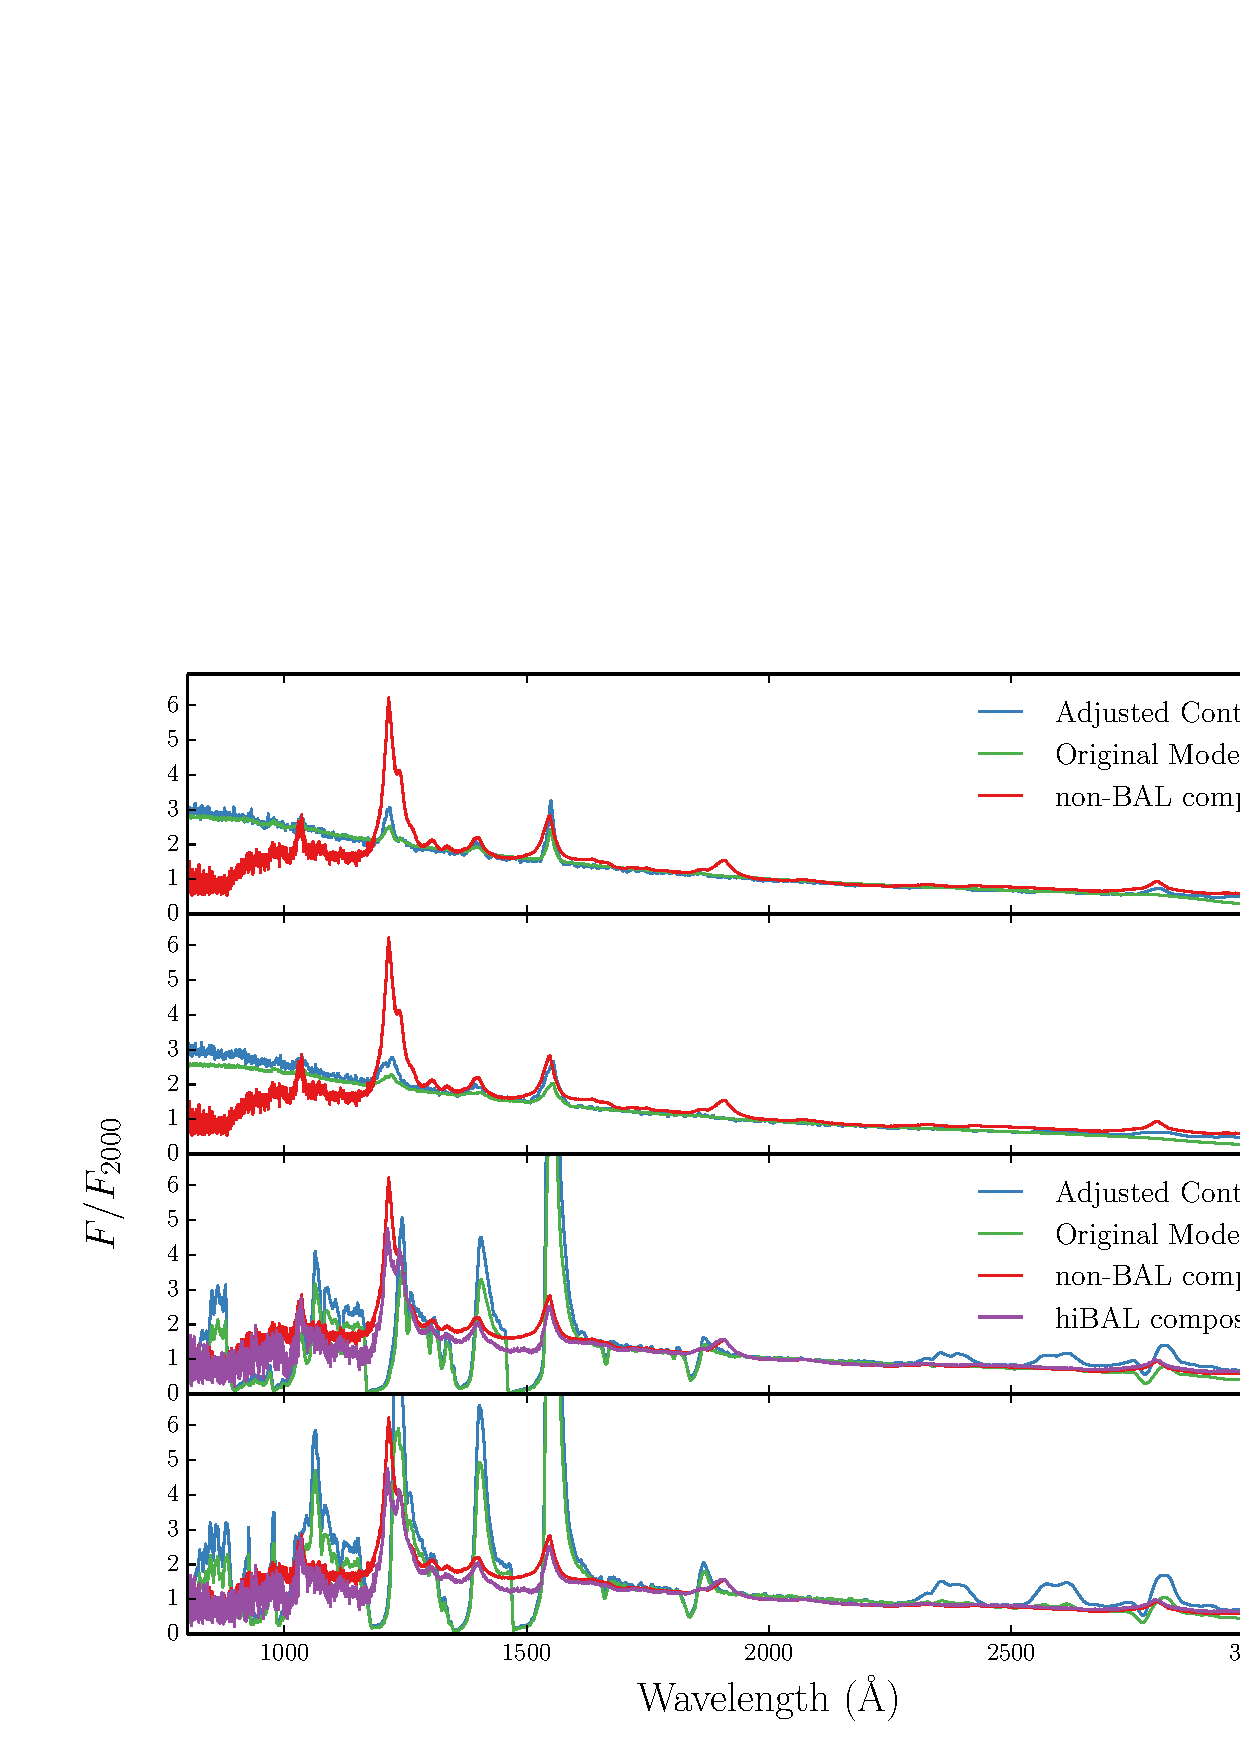
\includegraphics[width=1.0\textwidth]{figures/adjusted_withbals.png}
%DIF >  \caption
%DIF >  {
%DIF >  $F_\lambda$ normalised to $F_{2000}$. {\bf Again, this is a placeholder- but I'm thinking some kind of comparison to composite including the adjusted continuum, showing that we can't get it exactly right}.
%DIF >  }
%DIF >  \label{fig:finalcomp}
%DIF >  \end{figure*} %fullpage


%DIF >  \subsection{The BALQSO fraction and wind covering factor}
%DIF >  \label{sec:balfrac}

%DIF >  The disc SED has a profound effect on the intrinsic BAL fraction
%DIF >  inferred from flux-limited samples. This in turn impacts on 
%DIF >  the geometry and covering factor assumed for BALQSO and unified wind models,
%DIF >  and even effects the efficiency of feedback.
%DIF >  \cite{krolik1998} noted that the effect of limb darkening and foreshortening
%DIF >  would result in a signicantly underestimated covering factor for BALQSO winds.
%DIF >  The effect is complicated further by the quasar luminosity function -- if 
%DIF >  BALQSOs have lower observed luminosities for given accretion disc properties 
%DIF >  then they may be drawn from a different bin in the quasar luminosity function 
%DIF >  \citep{goodrich1997}. This will also have a similar impact
%DIF >  on the LoBALQSOs and FeLoBALQSOs sub-populations.
%DIF >  The complex (and as yet unknown) selection effects are understandably 
%DIF >  not taken into account by current estimates of the intrinsic BALQSO fraction 
%DIF >  \citep{weymann1991, reichard2003, knigge2008, turnermiller2009, allen2011}. 

%DIF >  The way forward is somewhat unclear. Given the lack of available observational 
%DIF >  constraints, models cannot readily be used to inform the selection criteria when 
%DIF >  calculating the BALQSO fraction. There are two main possibilities:
%DIF >  First, the disc emission is roughly isotropic, in which case the BAL fraction
%DIF >  estimates should be a good estimate of the covering factor of the outflow,
%DIF >  but the question about how this isotropy is achieved remains outstanding.
%DIF >  Or second, the disc emission is strongly anisotropic, which follows more
%DIF >  naturally from a disc geometry but has large implications
%DIF >  for the inferred covering factors, as well as leaving the similar line strengths
%DIF >  in BAL and non-BAL quasar compoosites unexplained (see previous sections).
%DIF >  Understanding the true nature of the disc SED, including the
%DIF >  angular distribution of radiation, is clearly crucial in order
%DIF >  to accurately estimate the true covering factor of BALQSO winds.

%DIF >  A brief comment, citing Goodrich / Krolik \& Voit on the 
%DIF >  way in which anisotropy / attenuation affect the inferred
%DIF >  BAL fraction. We also need to be aware that there will be a number of selection
%DIF >  effects in building up the composites, and we should discuss these
%DIF >  and the subtleties involved. 

%DIF >  \begin{figure}
%DIF >  \centering
%DIF >  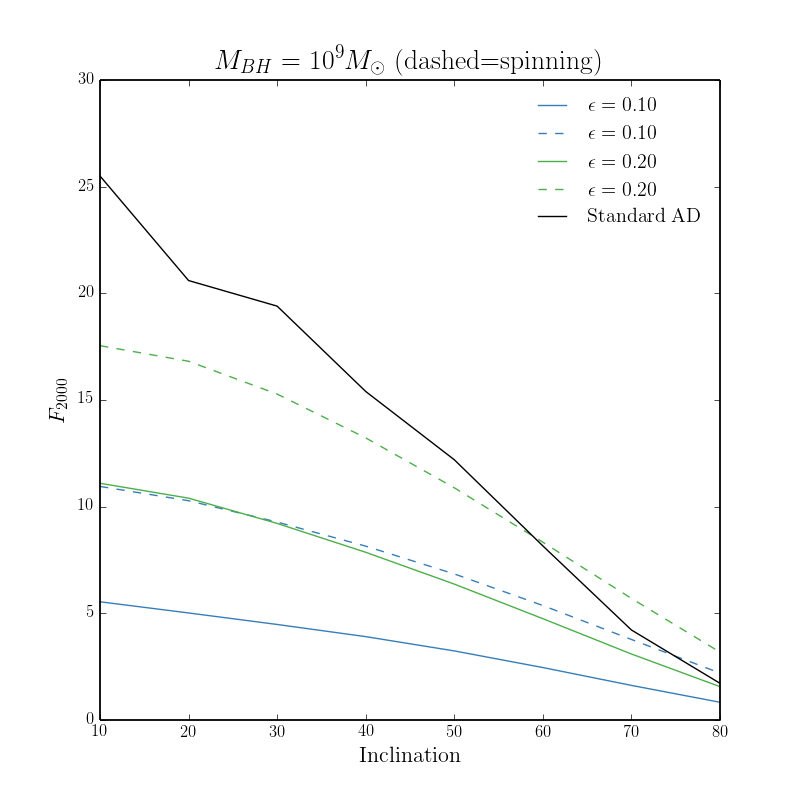
\includegraphics[width=0.45\textwidth]{figures/f2000_m9.png}
%DIF >  \caption
%DIF >  {
%DIF >  $F_\lambda$ at $2000$~\AA\ as a function of inclination from
%DIF >  \agn\ models. Spectra are computed for BH of $10^9~M_\odot$ with
%DIF >  a number of different BH spins and Eddington fractions. The black line
%DIF >  shows a standard multi-temperature blackbody AD model.
%DIF >  }
%DIF >  \label{fig:alpha_ox}
%DIF >  \end{figure}

%DIF > %%%%%%%%%%%%%%%%%%%%%%%%%%%%%%%%%%%%%%%%%%%%%%%%

\DIFaddend % SUMMARY

%%%%%%%%%%%%%%%%%%%%%%%%%%%%%%%%%%%%%%%%%%%%%%%%%

\section{Summary}

We have carried out MCRT simulations using a simple
prescription for a biconical disc wind, with
the aim of expanding on the work of H13 and assessing 
the viability of such a model for geometric unification of quasars.
We find the following main points:

\begin{enumerate}
\item We have introduced a first-order treatment 
of clumping in our model, and found that it can now maintain
the required ionization state while agreeing well with the X-ray
properties of AGN/QSOs.
\smallskip
\item We have shown that the degree of ionization stratification
in the model is sufficient that LoBAL line profiles
are seen at a subset of viewing angles, and Fe~\textsc{ii}
absorption is seen at particularly high inclinations.
\smallskip
\item We find that clumping also causes a significant 
increase in the strength of the  emission
lines produced by the model. This is true both
of collisionally excited resonance lines (such as \civ, \nv)
and recombination lines (such as \la, \ha\ and the Balmer series).
\smallskip
\item The line EWs in our models increase with inclination.
BAL and non-BAL quasar composites have comparable EWs, so our model
fails to reproduce this behaviour.
This is due to a fundamental constraint discussed further in section 5. If the BLR
emits fairly isotropically then for a foreshortened, limb-darkened classical thin accretion disc
it is simply not possible to achieve line ratios at low inclinations that are comparable to
those at high inclinations. This is a robust conclusion which 
is independent of the assumed BLR geometry and size.
\DIFdelbegin %DIFDELCMD < \smallskip
%DIFDELCMD < \item %%%
\DIFdel{We have examined the effect of GR on our disc SED, using the disc atmosphere
and GR ray-tracing code }%DIFDELCMD < \agn%%%
\DIFdel{. While including GR effects
does cause the disc SED to become slightly more isotropic,
the effect is not large enough to produce uniform line to continuum ratios
with viewing angle. We briefly discuss other solutions.
}\DIFdelend %DIF >  \smallskip
%DIF >  \item We have examined the effect of GR on our disc SED, using the disc atmosphere
%DIF >  and GR ray-tracing code \agn. While including GR effects
%DIF >  does cause the disc SED to become slightly more isotropic,
%DIF >  the effect is not large enough to produce uniform line to continuum ratios
%DIF >  with viewing angle. We briefly discuss other solutions.
\end{enumerate}
Our work confirms a number of expected outcomes from a geometric unification 
model, and suggests that a simple biconical geometry such as this can come close to 
explaining much of the  phenomenology of quasars. Nevertheless, our conclusions pose 
a clear challenge to the current disc wind unification picture.

%DIF >  To resolve these challenges, we suggest the following routes forward.
%DIF >  \begin{enumerate}
%DIF >  \smallskip
%DIF >  \item 
%DIF >  \smallskip
%DIF >  \item 
%DIF >  \smallskip
%DIF >  \item It is clear that the commonly accepted paradigm of an equatorial
%DIF >  wind with a covering factor of $\sim20\%$ does provide an adequate 
%DIF >  unified model, as shown here and by other authors 
%DIF >  (e.g. Marin \& Goosman 2013; DiPompeo et al. 2012a).
%DIF >  More collimated winds may solve some problems, but must be reconciled with
%DIF >  polarisation results that suggest an equatorial geometry.
%DIF >  Computing the polarisation of emergent energy packets in our 
%DIF >  MCRT code would allow direct comparison
%DIF >  between outputs from a known geometry and 
%DIF >  spectropolarimetry of quasars and AGN.
%DIF >  \smallskip
%DIF >  \item In addition to spectropolarimetry, one
%DIF >  of the best observational tools for probing outflow geometries
%DIF >  is reverberation mapping. We are starting to 
%DIF >  incorporate methods for predicting the reverberation
%DIF >  outputs from our models. By comparing with observational data, this
%DIF >  may provide stronger constraints on outflow geometries.
%DIF >  \end{enumerate}
\DIFaddbegin 






\DIFaddend \section*{Acknowledgements}

The work of JHM, SWM, NSH and \DIFdelbegin \DIFdel{CK }\DIFdelend \DIFaddbegin \DIFadd{CKL }\DIFaddend is supported by the
Science and Technology Facilities Council (STFC),
via two studentships and a consolidated grant, respectively.
\DIFaddbegin \DIFadd{CK also acknowledges a Leverhulme fellowship.
}\DIFaddend We would like to thank Omer Blaes, Ivan Hubeny and Shane Davis for their
assistance with \agn. We \DIFaddbegin \DIFadd{are grateful to Mike Brotherton, Mike DiPompeo,
Sebastien Hoenig and Frederic Marin for helpful correspondence regarding
polarisation measurements and orientation indicators.
We }\DIFaddend would also like to thank Daniel Proga, Daniel Capellupo, Sam Connolly and
Dirk Grupe for useful discussions.  Simulations were conducted using \py\ version \DIFdelbegin \DIFdel{79c}\DIFdelend \DIFaddbegin \DIFadd{80}\DIFaddend ,
and made use of the IRIDIS High Performance Computing Facility at the
University of Southampton. Figures were produced using \DIFaddbegin \DIFadd{the }\DIFaddend {\tt matplotlib} \DIFaddbegin \DIFadd{plotting library
}\DIFaddend \citep{matplotlib}.


%% \texttt{mn2e.cls} \textsc{Latex} document class. 

\bibliography{mybib.bib,stellar.bib,h14.bib,h13.bib,hamann.bib,krolik.bib}
\clearpage
\clearpage
%\appendix
% \appendix
% \section{Notes}
\DIFdelbegin %DIFDELCMD < 

%DIFDELCMD < %%%
%DIF <  Here are some notes on various parts of the text.
%DIF <  \smallskip
%DIFDELCMD < 

%DIFDELCMD < %%%
%DIF <  \begin{itemize}
%DIF <  	\item 
%DIF <  	\item Figure 3 should be improved to include some kind of real colormap of the model
%DIF <  	\item At the moment I haven't included another plot for the optical spectrum, or discussed
%DIF <  	it in the paper.
%DIF <  	\item Figure 5 needs to show a sample at the higher luminosity end, and include the actual relationship as the dotted line instead of a by eye version as is currently 
%DIF <  	\item
%DIF <  	\item
%DIF <  	\item
%DIF <  	\item
%DIF <  	\item
%DIF <  	\item
%DIF <  	\item
%DIF <  \end{itemize}
\DIFdelend 


\end{document}
